%%% index.tex -- Generico contenitore per matematica in lingua inglese.
%%%
%%% $Id: index.tex,v 1.4 2006/05/12 11:00:59 rmurri Exp $
%%%
\documentclass[a4paper,reqno,openany,draft]{amsbook}

%%%
%%% DEBUG!
%%%
\usepackage{debug} % debugging code
%\usepackage[outline]{draftcopy}
\usepackage{rcs}
%\def\RCSID$#1${}

%%%
%%% NOTAZIONI MATEMATICHE
%%%

%%
%% Theorems, Lemmas, and the like...
%%
\usepackage{amsthm}
\providecommand{\theoremname}{Theorem}

\newtheorem{theorem}{Theorem}[chapter]
\newtheorem*{theorem*}{Theorem}
\newtheorem{thmsec}{Theorem}[section]
\newtheorem{lemma}{Lemma}[section]
\newtheorem{proposition}[theorem]{Proposition}
\newtheorem{claim}{Claim}[chapter]
\newtheorem{conjecture}{Conjecture}[chapter]
\newtheorem{corollary}[theorem]{Corollary}

\theoremstyle{remark}
\newtheorem{remark}{Remark}[section]
\newtheorem*{ack}{Acknowledgments}
\newtheorem*{notations}{Notations}

\theoremstyle{definition}
\newtheorem{definition}{Definition}[section]
\newtheorem{example}{Example}[chapter]

\numberwithin{equation}{section} % numerazione delle equazioni

%%
%% Notazioni matematiche di *questo* articolo
%%
\usepackage{miscmath} % simboli vari

\renewcommand\k\fk
\renewcommand\d\ud

\newcommand{\A}{\category{A}}     % generic category A
\newcommand{\B}{\category{B}}     % generic category B
\newcommand{\rev}{\sptext{rev}}
\newcommand{\catN}{\category{N}}        % generic category N
\newcommand{\Oo}[1][]{\operad{O}_{#1}}  % generic operad O
\newcommand{\RTD}[1][]{\operad{D}_{#1}} % operad of RT diagrams
\newcommand{\RTE}[1][]{\operad{D}'_{#1}}% operad of embedded RT graphs
\newcommand{\RTG}[1][]{\operad{G}_{#1}} % operad of RT graphs
\newcommand{\RG}[1][]{\operad{R}_{#1}}  % operad of cyclic (Ribbon) graphs
\newcommand{\SG}[1][]{\operad{S}_{#1}}  % operad of symmetric graphs
\newcommand{\freemc}[1]{#1^{\otimes}}   % free monoidal category 
\newcommand{\freemsc}[1]{#1^{\Box}}     % free monoidal signed category 
\newcommand{\tpc}[1]{\langle #1 \rangle}% tensor powers category
\newcommand{\btpc}[1]{\langle#1\rangle^+}% (bosonic) tensor powers category
\newcommand{\ftpc}[1]{\langle#1\rangle^-}% (fermiionic) tensor powers ctg.

\newcommand{\Strebel}[1][]{\mathcal{S}_{#1}}
\newcommand{\Conf}{\text{\rm Conf}}
\newcommand{\T}{\mathcal{T}}
\newcommand{\Lb}{\mathcal{L}}
\newcommand{\Hn}{\mathcal{H}}

% decomposizione cellulare dei grafi a nastro
\newcommand{\Vertices}[1]{#1^{(0)}}
\newcommand{\Edges}[1]{#1^{(1)}}
\newcommand{\Holes}[1]{#1^{(2)}}

% medie sui grafi
\newcommand{\vv}[1]{V(#1)}
\newcommand{\biggint}[2][]{%
\Biggl\langle\Biggl\langle#2\Biggr\rangle\Biggr\rangle_{#1}}
\newcommand{\gint}[2][]{%
  \left\langle\!\left\langle#2\right\rangle\!\right\rangle_{#1}}
\newcommand{\ginttriv}[2][]{%
  \left\langle\!\left\langle#2\right\rangle\!\right\rangle_{#1}\triv}

% omotopia
\newcommand{\rel}{\sim}

%%
%% `xy' --- grafica
%%
\usepackage[ps,dvips,xdvi,colour,all,arc,knot,poly]{xy}
\everyxy={/r24pt/:} % scala per i diagrammi
\def\xyc#1\endxyc{\xy*!LC\xybox{#1}\endxy}

\usepackage{rg} % vertici e buche di grafi a nastro

%%
%% `paralist' -- Miglior supporto per le liste
%%
\usepackage[newitem,newenum]{paralist}
\setdefaultenum{\slshape 1)}{\slshape a)}{\slshape i)}{A.}
%\defaultitem{$\triangleright$}{}{}{}

%%
%% `mdwlist' -- \suspend / \resume list environments
%%
\usepackage{mdwlist}

%%
%% `mdwtab' -- better support for tables
%%
\usepackage{mdwtab}

%%
%% `url' -- Inserimento di URL
%%
\usepackage{url}

%%
%% `hyperref' -- Collegamenti ipertestuali
%%
\usepackage{hyperref}

%%
%% `nomencl' -- Indice delle notazioni
%%

\usepackage[refpage]{nomencl} % indice dei simboli
\let\nx=\nomenclature
\makeglossary % per l'indice dei simboli

%%
%% `csref' -- genera automaticamente il nome di un riferimento.
%%
\usepackage{csref}

%%
%% `graphicx' -- inclusione di grafica esterna
%%
\usepackage[final]{graphicx}


%%%
%%% Cominciamo...
%%%
%\includeonly{kontsevich,construction}
\begin{document}

\RCSID $Id: title.tex,v 1.4 2003/06/23 17:38:08 murri Exp $
%auto-ignore


\title{To be continued}
\date{2001-12-21}
\author{Riccardo Murri}
\address{%
  Scuola Normale Superiore \\
  p.za dei Cavalieri, 7 \\
  56127 Pisa \\
  Italy
  }
\email{riccardo.murri@gmx.it}

%\subjclass{To be determined}
%\begin{abstract}
%\end{abstract}
\maketitle

\setcounter{tocdepth}{2} % fino a profondit{\`a} di \section

\tableofcontents

%%% Local Variables: 
%%% mode: latex
%%% TeX-master: "index"
%%% End: 

\RCSID $Id: prelim.tex,v 1.4 2006/05/12 11:00:59 rmurri Exp $
%auto-ignore


\chapter{Preliminaries and Notation}

This chapter fixes some notations on differential graded modules
and categories.\FIXME{Rimuovere del tutto questo paragrafo?}

When $\A$ is a category, we shall use Eilenberg's $\A(A, B)$ in place
of the more verbose $\Hom \A(A, B)$.  By abuse of notation, we write
$A \in \A$ to mean that ``$A$ is an object of $\A$''. Often, the
notation $\Hom\A$ will be used for the union of all the $\Hom$-sets of
the category $\A$, i.e., $\Hom\A := \bigcup_{A,B \in \A} \A(A,B)$.  The words
``morphism'', ``map'' and ``arrow'' will be used interchangeably.

The symbol $\Perm{k}$ stands for the group of permutations on $k$
letters.

The degree $i$ component of a graded object $M^\#$ will be denoted
$M^i$; the grading group will always be $\setZ$. Elements of a graded
object appearing as exponents to a number will stand for their degree,
i.e., $(-1)^a := (-1)^{\deg a}$; hence, $(-1)^{ab} \not=
(-1)^{\deg (ab)} = (-1)^{\deg a + \deg b} = (-1)^{a+b}$.


\section{Differential graded algebras and modules}
\label{sec:dg-things}

Let $\fk$ be a fixed field of characteristics $0$; later on, we shall
assume $\fk = \setC$.
\begin{definition}
  A dg-algebra $K$ consists of a graded vector space $K^\#$ over $\fk$,
  a $\fk$-bilinear associative product, and a $\fk$-linear map $\ud:
  K\to K$ such that:
  \begin{enumerate}
  \item $K^i \cdot K^j \subset K^{i+j}$;
  \item $ab = (-1)^{ab} ba$ (graded commutativity);
  \item $\ud(K^i) \subset K^{i+1}$;
  \item $\ud(a\cdot b) = \ud(a)\cdot b + (-1)^a a\cdot\ud(b)$ (graded Leibniz rule).
  \end{enumerate}
  Furthermore, we shall always assume that a dg-algebra has a unit
  $1\in K^0$ such that $1\cdot a = a\cdot 1 = a$ for all $a\in
  K$.
\end{definition}

Any dg-algebra is a (graded) associative commutative algebra.

\begin{definition}
  A $K$-dg-module $M$ is a $K$-bimodule such that:
  \begin{enumerate}
  \item $K^i M^j \subset M^{i+j}$, $M^i K^j \subset M^{i+j}$;
  \item $\lambda x = (-1)^{\lambda x} x\lambda$, for all homogeneous
    $x\in M$, and $\lambda\in K$;
  \item $\ud(\lambda x) = \ud(\lambda)x + (-1)^\lambda \lambda\ud(x)$.
  \end{enumerate}
\end{definition}

There is an obvious underlying functor $\#$ that ``forgets the
differential'', from the category of $K$-dg-modules to the category of
$K$-modules.

\begin{definition}
  For every two $K$-dg-modules $M$, $N$ we define the module of
  degree $p$ morphisms
  \begin{equation*}
    \Hom_K^p (M,N) := \Bigl\{ f\in  {\textstyle \prod_i} Hom_\fk (M^i, N^{i+p}) :
      f(x\lambda) = f(x)\lambda \quad \forall x\in M, \forall \lambda
      \in R \Bigr\},
  \end{equation*}
  and the graded module of morphisms
  \begin{equation*}
    \Hom_K^* := \oplus_{p\in\setZ} \Hom_K^p (M,N)[-p],
  \end{equation*}
  that is, $\Hom_K^p(M,N)$ is the degree $p$ component of
  $\Hom_K^*(M,N)$.
\end{definition}

$\Hom_K^*(M,N)$ is made into a $K$-dg-module by the differential:
\begin{equation*}
  \ud f := \ud_N \circ f + (-1)^{p+1} f\circ \ud_M \qquad f\in \Hom_K^p(M,N)
\end{equation*}
The term ``morphism'' will denote any element of $\Hom_K^*$, whereas
``dg-morphism'' will be applied only to those such that $\ud f = 0$.


\section{Braided symmetric categories of Modules}
\label{sec:btc+dg}

Given any commutative dg-algebra $K$, the category $\catMod_K^\setZ$ of
finitely-generated $K$-dg-bimodules is in a natural way braided and
balanced with the structure maps:
\begin{align}
  \label{eq:dgm-braiding}
  \tau_{MN} &: M \otimes N \ni m\otimes n \mapsto (-1)^{mn}n\otimes m \in N \otimes M
  &&
  \text{(braiding),}
  \\
  \label{eq:dgm-balancing}
  \theta_M &: M \ni m \mapsto (-1)^mm \in M
  &&
  \text{(balancing).}
\end{align}
The verification that these maps satisfy the axioms of a balanced
braided symmetric category is an easy calculation.  The usual
definition of the dual object $\rdl{M} := \Hom_K(M, K)$ gives an
obvious evaluation map $\ev_M : M \otimes \rdl{M} \ni m \otimes \rdl{m} \mapsto
\pairing{m}{\rdl{m}} \in K$, but one cannot generally assert the
existence of a matching coevaluation morphism unless $M$ is a free
module.

The above structure maps
\eqref{eq:dgm-braiding}--\eqref{eq:dgm-balancing} induce a balanced
symmetric braided category structure on the subcategory $\catMod_K$ of
degree $0$ $K$-bimodules; the braiding on $\catMod_K$ restricts to the
trivial one: $\tau_{MN}: m\otimes n \mapsto n\otimes m$.
\begin{remark}
  In fact, Eilenberg and Kelly \cite{eilenberg-kelly;monoidal-categories}
  show that there are just two possible braidings on $\catMod_K^\setZ$:
  the trivial one given by:
  \begin{equation*}
    \tau_{MN}^+ : m\otimes n \mapsto n\otimes m,
  \end{equation*}
  which is the usual braiding on categories of non-graded modules and
  vector spaces, and and that of \eqref{eq:dgm-braiding},
  \begin{equation*}
    \tau_{MN}^- : m\otimes n \mapsto (-1)^{mn} n\otimes m,
  \end{equation*}
  which is the usual one on categories of graded modules.
\end{remark}


\section{Signs and the graded contraction}
\label{sec:signs}

Recall that the symmetric monoidal category of graded modules has a
non-trivial (yet involutive) braiding isomorphism
\begin{equation*}
\tau_{(12)} = \tau_{M_1M_2} : M_1
\otimes M_2 \ni x_1\otimes x_2 \mapsto (-1)^{x_1x_2} x_2\otimes x_1
\in M_2\otimes M_1,
\end{equation*}
for all objects $M_1$, $M_2$.  Any $\sigma\in\Perm{n}$ has a decomposition
into a product of traspositions $(ij)$; since the category of graded
modules is sysmmetric, we can define an isomorphism $\tau_\sigma: M_1 \otimes \cdots \otimes
M_n \to M_{\sigma_1} \otimes \cdots \otimes M_{\sigma_n}$ as the composition of twists $\tau_{(ij)}$;
$\tau_\sigma$ does not depend on the chosen factorization of $\sigma$ into
traspositions.

Now, suppose $M_1 = \dots = M_n = M$, a fixed object: $x_1\otimes \dots \otimes
x_n$ and $\tau_\sigma(x_1\otimes \dots \otimes x_n)$ differ only by the sign; therefore we
define the Koszul sign $\epsilon(\sigma; x_1, \dots, x_n)$ so that the following
holds:
\begin{equation}
  \label{eq:ksz}
  \epsilon(\sigma; x_1, \dots, x_n) x_1 \otimes \dots \otimes x_n =
  \tau_\sigma (x_1 \otimes \dots \otimes x_n), \qquad \sigma\in\Perm{n}.
\end{equation}
Also define the alternating Koszul sign $\chi(\sigma; x_1, \ldots, x_n)$ by:
\begin{equation}
  \label{eq:aksz}
  \chi(\sigma; x_1, \dots, x_n) x_1 \otimes \dots \otimes x_n =
  (-1)^\sigma \varepsilon(\sigma; x_1, \ldots, x_n)
  \qquad \sigma\in\Perm{n}.
\end{equation}
We shall omit $x_1, \dots, x_n$ from the above when it will be clear
from the context which elements $\epsilon$ or $\chi$ are being
applied to.

\begin{definition}\label{dfn:graded-sym-map}
  A map $f: M^{\otimes n} \to N$ is graded symmetric iff
  \begin{equation*}
    f(x_1, \dots, x_n) = \epsilon(\sigma) f(x_{\sigma_1}, \dots,
    x_{\sigma_n}) \qquad \forall x_1, \dots, x_n \in M.
  \end{equation*}
  It is graded antisymmetric iff
  \begin{equation*}
    f(x_1, \dots, x_n) = \chi(\sigma) f(x_{\sigma_1}, \dots,
    x_{\sigma_n}) \qquad \forall x_1, \dots, x_n \in M.
  \end{equation*}
\end{definition}

Since permutation of factors in a tensor product may change the sign,
the contraction map 
\begin{equation*}
c: {\textstyle \bigotimes_i} \Hom(M_i, N_i) \otimes
 {\textstyle \bigotimes_i} M_i \to  {\textstyle \bigotimes_i} N_i
\end{equation*}
is well-defined only up to a sign. In search of a remedy, we fix an
ordering of the factors which gives ``unsigned'' contraction, and then
define contraction of any permutation of the factors
$\left\{\Hom(M_i,N_i), M_i\right\}_{i\in I}$ by first applying a twist
$\tau_\sigma$ to get the fixed ``standard'' ordering, and then the usual
``unsigned'' contraction. Formally:
\begin{enumerate}
\item let $c: \Hom(M,N) \otimes M \ni f\otimes x \mapsto f(x) \in N$;
\item let $c: \bigotimes_i (\Hom(M_i, N_i) \otimes M_i) \ni (f_1\otimes x_1)
  \otimes \dots (f_k\otimes x_k) \mapsto f_1(x_1) \otimes \dots
  \otimes f_k(x_k) \in \bigotimes N_i$;
\item let $W_{2i-1} := \Hom(M_i, N_i)$, $W_{2i} := M_i$, for $i =
  1, \dots, k$; define the contraction
  \begin{equation*}
    c: {\textstyle \bigotimes_{j=1}^{2k}} W_{\sigma_j} \to
    {\textstyle \bigotimes_{i=1}^k} N_i
  \end{equation*}
  by 
  \begin{equation*}
    {\textstyle \bigotimes_{j=1}^{2k}} W_{\sigma_j} \to {\textstyle \bigotimes_{j=1}^{2k}} W_j \to
    {\textstyle \bigotimes_{i=1}^{k}} N_i.
  \end{equation*}
\end{enumerate}

Infact, this boils down to the rule: ``change the sign by
$(-1)^{pq}$ when interchanging objects of degree $p$ and $q$''.


\section{Braided symmetric categories of vector spaces}
\label{sec:btc-vect}

The categories of ($\setZ$-graded) $\fk$-linear spaces, $\catVect[\fk]^\setZ$
and $\catVect[\fk]$ have natural structures of symmetric braided
autonomous tortile category if we consider $\fk$ to be a
$\fk$-dg-algebra concentrated in degree $0$.

However, every vector space is a free module, so, for any $V \in
\catVect^\setZ$, pick a base $(v_i)$ and a dual base $(\rdl{v_i})$ of
$\rdl{V}$ such that $\pairing{v_i}{\rdl{v_j}} = \delta_{ij}$; we can
define evaluation and coevaluation maps
\begin{align}
  \label{eq:vec-evaluation}
  \ev_V &: v \otimes \rdl{v} \mapsto \pairing{v}{\rdl{v}}, 
  \\
  \label{eq:vec-coevaluation}
  \coev_V &: 1 \mapsto \sum_i \rdl{v_i} \otimes v_i,
\end{align}
which make $\catVect^\setZ$ into an autonomous category; these morphisms
are actually independent of the chosen basis $(v_i)$. The balancing
map \eqref{eq:dgm-balancing} is compatible with taking duals, so
$\catVect^\setZ$ is a tortile category.
\begin{remark}\label{rem:ev-rev}
  \FIXME{{\`E} coerente con la regola dei segni data sopra?  Sembra di s{\`\i},
  ma allora non c'{\`e} differenza\ldots}
  Note that, although $V^{\lor\lor} \simeq V$, the reverse-order evaluation
  and coevaluation maps $\ev'_V$, $\coev'_V$ differ from
  $\ev_{\rdl{V}}$ and $\coev_{\rdl{V}}$ by a sign, because of the
  non-trivialness of $\tau_{V,\rdl{V}}$; indeed, according to
  \ref{thm:ev-rev},
  \begin{align*}
    \ev'_V = \ev_V \circ \tau_{V,\rdl{V}} &: \rdl{v} \otimes v \mapsto (-1)^{v\rdl{v}}
    \pairing{v}{\rdl{v}},
    \\
    \ev_{\rdl{V}} &: \rdl{v} \otimes v \mapsto \pairing{\rdl{v}}{v},
  \end{align*}
  and similarly $\coev'_V = \pm \coev_{\rdl{V}}$.
\end{remark}

The category $\catVect$ of degree $0$ vector spaces inherits a
structure of a tortile autonomous braided symmetric category from
$\catVect^\setZ$, but the braiding restricts to the trivial one.


\subsection{The category of Bosonic states}
\label{sec:bosonic}
\nx{\btpc{V,b}}{Category of Bosonic states}

Let $V$ be a $\fk$-vector space equipped with a bilinear
\emph{symmetric} non-degenerate form $b: V\tp{2} \to \fk$. Let
$\btpc{V,b}$ be the full subcategory of $\catVect$ which has tensor
powers $V\tp{p}$ as objects; $\btpc{V,b}$ inherits a balanced
symmetric tensor structure from $\catVect$. For each $V\tp{p} \in
\btpc{V,b}$ define maps
\begin{equation*}
  \ev_{V\tp{p}}: V\tp{p} \otimes V\tp{p} \ni (v_1, \ldots, v_p) \otimes (v'_1, \ldots, v'_p) \mapsto
  b(v_1, v'_1) \cdots b(v_p, v'_p) \in \fk \simeq I.
\end{equation*}
Since $b$ is non-degenerate and $V$ is finite-dimensional, $\ev^\sharp$ is
a linear isomorphism, hence a bijection, so $V\tp{p}$ is a self-dual
object and $\btpc{V,b}$ is an autonomous category.

The category $\btpc{V,b}$ can be used as a base for a graphical
calculus description of Feynman diagrams associated to Gaussian
integrals --- see \cite[sec.\
2.8]{murri-fiorenza;feynman}.\FIXME{Piccolo spazio pubblicit{\`a}\ldots}



%%% Local Variables: 
%%% mode: latex
%%% TeX-master: "index"
%%% x-symbol-8bits: nil
%%% End: 

\RCSID $Id: gc.tex,v 1.1.1.1 2002/01/10 10:01:51 ri Exp $
%auto-ignore


\chapter{The Graphical Formalism for Symmetric Tensor Categories}
\label{cha:gc}

The graphical formalism for braided tensor categories was developed in
the late 1980's, when a categorical formulation of polynomial knot
invariants was given \cite{freyd-yetter;btc, turaev;yang-baxter}.
After this discovery, braided tensor categories were recognized as a
``reasonably general setting'' \cite{joyal-street;tensor-calculus}
where the graphical notation for tensors ---which, infact, dates back
to Penrose's \cite{penrose;negative-dimensional-tensors}--- could be
given firm grounds and a well-defined meaning.

This line of research culminated in
\cite{joyal-street;tensor-calculus}, where it is shown how
the gradually enriching the structure of a category beyond the
braiding leads to gradually enriching the corresponding graphs, and
\cite{reshetikhin-turaev;ribbon-graphs}, where the final case of
autonomous tortile categories is settled.

I will not attempt here to give proofs of these results, but rather
derive the needed rather simple instances of graphical calculus as a
corollary to the most general results of Reshetikhin and Turaev.
However, proper statement of these requires quite a long preamble of
category-related material; I would therefore just skim over the
necessary definitions, and refer the interested reader \csref{cha:rt}
and~\ref{cha:btc} for precise statements, and to the foundational
papers of Joyal and Street \cite{joyal-street;tensor-calculus,
  joyal-street;btc} for details, proofs, motivation and history.

As terminology in these matters is not yet generally agreed upon, I
will adhere to nomenclature used by Joyal and Street in
\cite{joyal-street;tensor-calculus, joyal-street;btc}. All relevant
definitions are grouped in \csref{cha:btc}.


\section{Graphical formalism for Symmetric Tensor Categories}
\label{sec:gc-stc}
\FIXME{In tutto questo capitolo, gli spazi di morfismi sono in verit{\`a}
  gli span lineari di quelli che sono veramente descritti\ldots}
Let $\A$ be a symmetric autonomous tortile category. For an object $A
\in \A$, let $A^{-1} := \rdl{A}$ and $A^{+1} := A$.
\begin{definition}\label{dfn:gc-graph-piece}
  An $\A$-colored elementary diagram piece is any one of the
  following:
  \begin{center}
    \begin{tabular}{cccccc}
      $\xy*!LC\xybox{(0,0)*+{A};(0,1)*+{A}**\dir{-}}\endxy$
      &
      $\xy*!LC\xybox{%
        \vcross~{(0,1)*+{B}}{(1,1)*+{A}}{(0,0)*+{A}}{(1,0)*+{B}}}\endxy$
      &
      $\xy*!LC\xybox{%
        \vcross~{(0,0)*+{B}}{(1,0)*+{A}}{(0,1)*+{A}}{(1,1)*+{B}}}\endxy$
      &
      $\xy*!LC\xybox{%
        \vloop~{(0,1)}{(1,1)}{(0,0)*+{A}}{(1,0)*+{A}}}\endxy$
      &
      $\xy*!LC\xybox{%
        \vloop~{(0,0)}{(1,0)}{(0,1)*+{A}}{(1,1)*+{A}}}\endxy$
      &
      $\xy*!LC\xybox{
        (0,1)*+[F]{f};%
        (-1,0)*+{A_1}**\dir{-},(-0.5,0)*+{A_2}**\dir{-},%
        (0,0.5)*+{\ldots},(1,0)*+{A_r}**\dir{-},%
        (-1,2)*+{B_1}**\dir{-},(-0.5,2)*+{B_2}**\dir{-},%
        (0,1.5)*+{\ldots},(1,2)*+{B_s}**\dir{-},%
        }\endxy$
      \\
      (a) & (b) & (c) & (d) & (e) & (f)
    \end{tabular}
  \end{center}
  For each strand $\ell$, some additional structure is specified:
  \begin{itemize}
  \item an object of $\A$;
  \item a sign $\varepsilon_\ell$, that is, an orientation;
  \item a framing, that is, a map $N_\ell: [0,1] \to S^1$ such that
    $N_\ell(0) = N_\ell(1) = 1$.
  \end{itemize}
  
  Additionally, each piece of type (f) is decorated by a morphism $f
  \in \Hom\A$: if $\epsilon_1$, \ldots, $\epsilon_r$, $\eta_1$, \ldots, $\eta_s$ are the signs
  on the upper and lower strands of a piece of type (f), then $f \in
  \A(A_1^{\epsilon_1} \otimes \cdots \otimes A_r^{\epsilon_r}, B_1^{\eta_1} \otimes \cdots \otimes B_s^{\eta_s})$.
\end{definition}
A piece of type (a) is called a ``strand''; those of type (b) and (c)
are named ``crossings''; (d) and (e) are the ``coupling'' and the
``Casimir''; (f) is, plainly, a ``vertex''. The size of the rectangle
in a piece of type (f) is really immaterial.

We say the free strands at the bottom are ``input legs'' and those at
the top are ``output legs''. For a given piece $v$ of type (f), define
\begin{gather*}
  \Src(v) := A_1^{\epsilon_1} \otimes \cdots \otimes A_r^{\epsilon_r},
  \\
  \Tgt(v) := B_1^{\eta_1} \otimes \cdots \otimes B_r^{\eta_s},
\end{gather*}
if the $r$ input strands are decorated by objects $A_1$, \ldots, $A_r$ and
signs $\epsilon_1$, \ldots, $\epsilon_r$, while the $s$ output strands are decorated
by objects $B_1$, \ldots, $B_s$ and signs $\eta_1$, \ldots, $\eta_s$.

One can compose graph pieces $\Gamma_1$ and $\Gamma_2$ by stacking one on top
of the other (see \csref{fig:gc-graph-composition}), if $\Src(\Gamma_1) =
\Tgt(\Gamma_2)$, i.e., the input legs of $\Gamma_1$ match the output legs of
$\Gamma_2$ in number, color, orientation, and framing. The tensor product
of two graph pieces $\Gamma_1$ and $\Gamma_2$ is defined by juxtaposition, as
in \csref{fig:gc-graph-otimes}; note that no compatibility condition
is required in this case. We have the following
\begin{align}
  \label{eq:src-comp-otimes}
  \Src(\Gamma_1 \circ \Gamma_2) &= \Src(\Gamma_2), 
  &&
  \Src(\Gamma_1 \otimes \Gamma_2) &= \Src(\Gamma_1) \otimes \Src(\Gamma_2),
  \\
  \label{eq:tgt-comp-otimes}
  \Tgt(\Gamma_1 \circ \Gamma_2) &= \Tgt(\Gamma_1),
  &&
  \Tgt(\Gamma_1 \otimes \Gamma_2) &= \Tgt(\Gamma_1) \otimes \Tgt(\Gamma_2).
\end{align}

We give the definition of the category of graphs in the arrows-only
form (see \csref{cha:arrows}). 
\begin{definition}
  The $\A$-colored diagrams category $\RTD[\A]$ is the category whose
  morphisms are generated from $\A$-colored elementary pieces thorugh
  the operations of graph composition and tensor product, defined as
  in figures~\ref{fig:gc-graph-composition}
  and~\ref{fig:gc-graph-otimes}.
  
  The $\A$-colored graph category $\RTE[\A]$ is the category whose set
  of morphisms is the quotient of $\Hom\RTD[\A]$ by the
  Reidmeister-Reshetikhin-Turaev relations of \csref{fig:gc-rrt}.
\end{definition}
%% Figura 1
\begin{figure}[p]
  \centering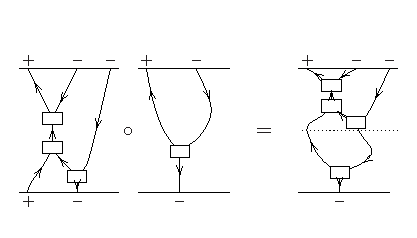
\includegraphics{fig-001}
  \caption{Composition product of diagrams.}
  \label{fig:gc-graph-composition}
\end{figure}
%% Figura 2
\begin{figure}[p]
  \centering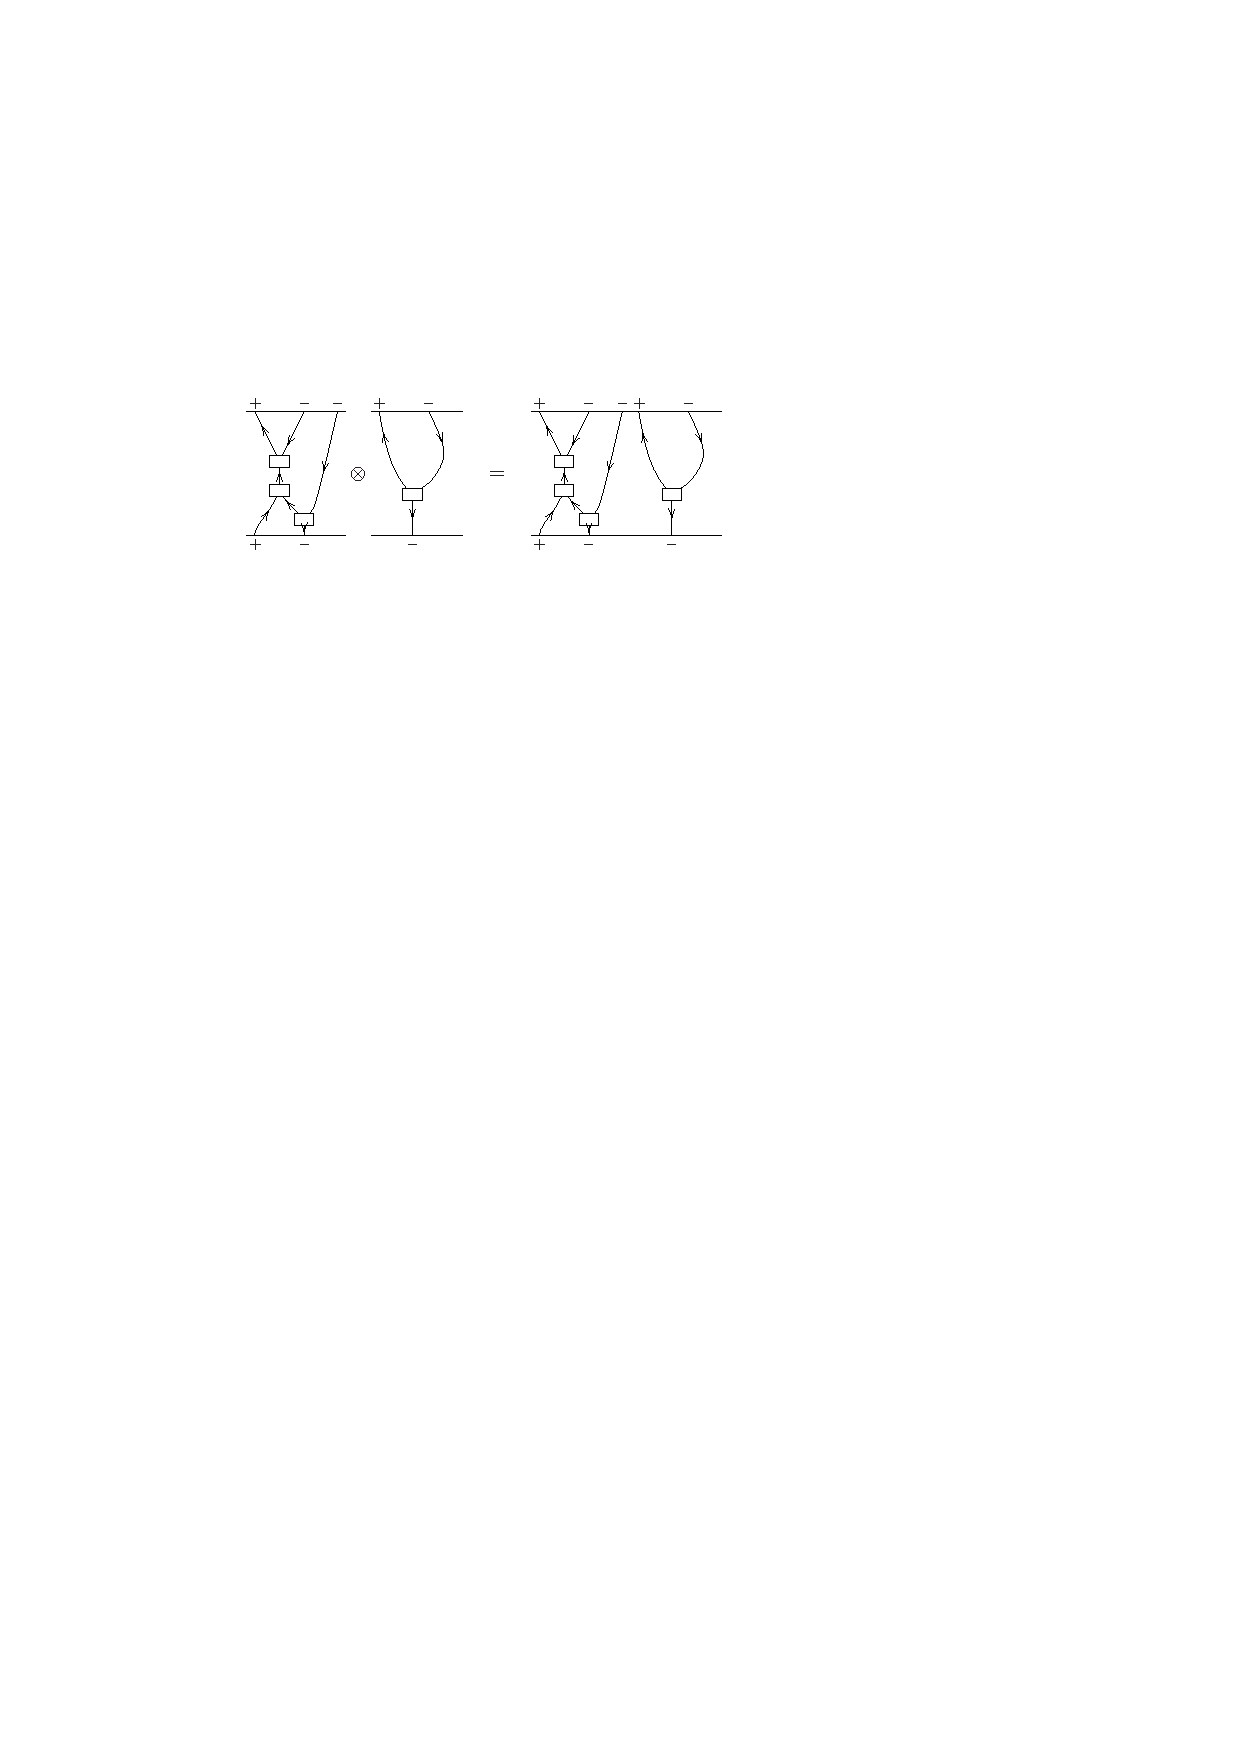
\includegraphics{fig-002}
  \caption{Tensor product of diagrams.}
  \label{fig:gc-graph-otimes}
\end{figure}
%% Figura 3
\begin{figure}[p]
  \centering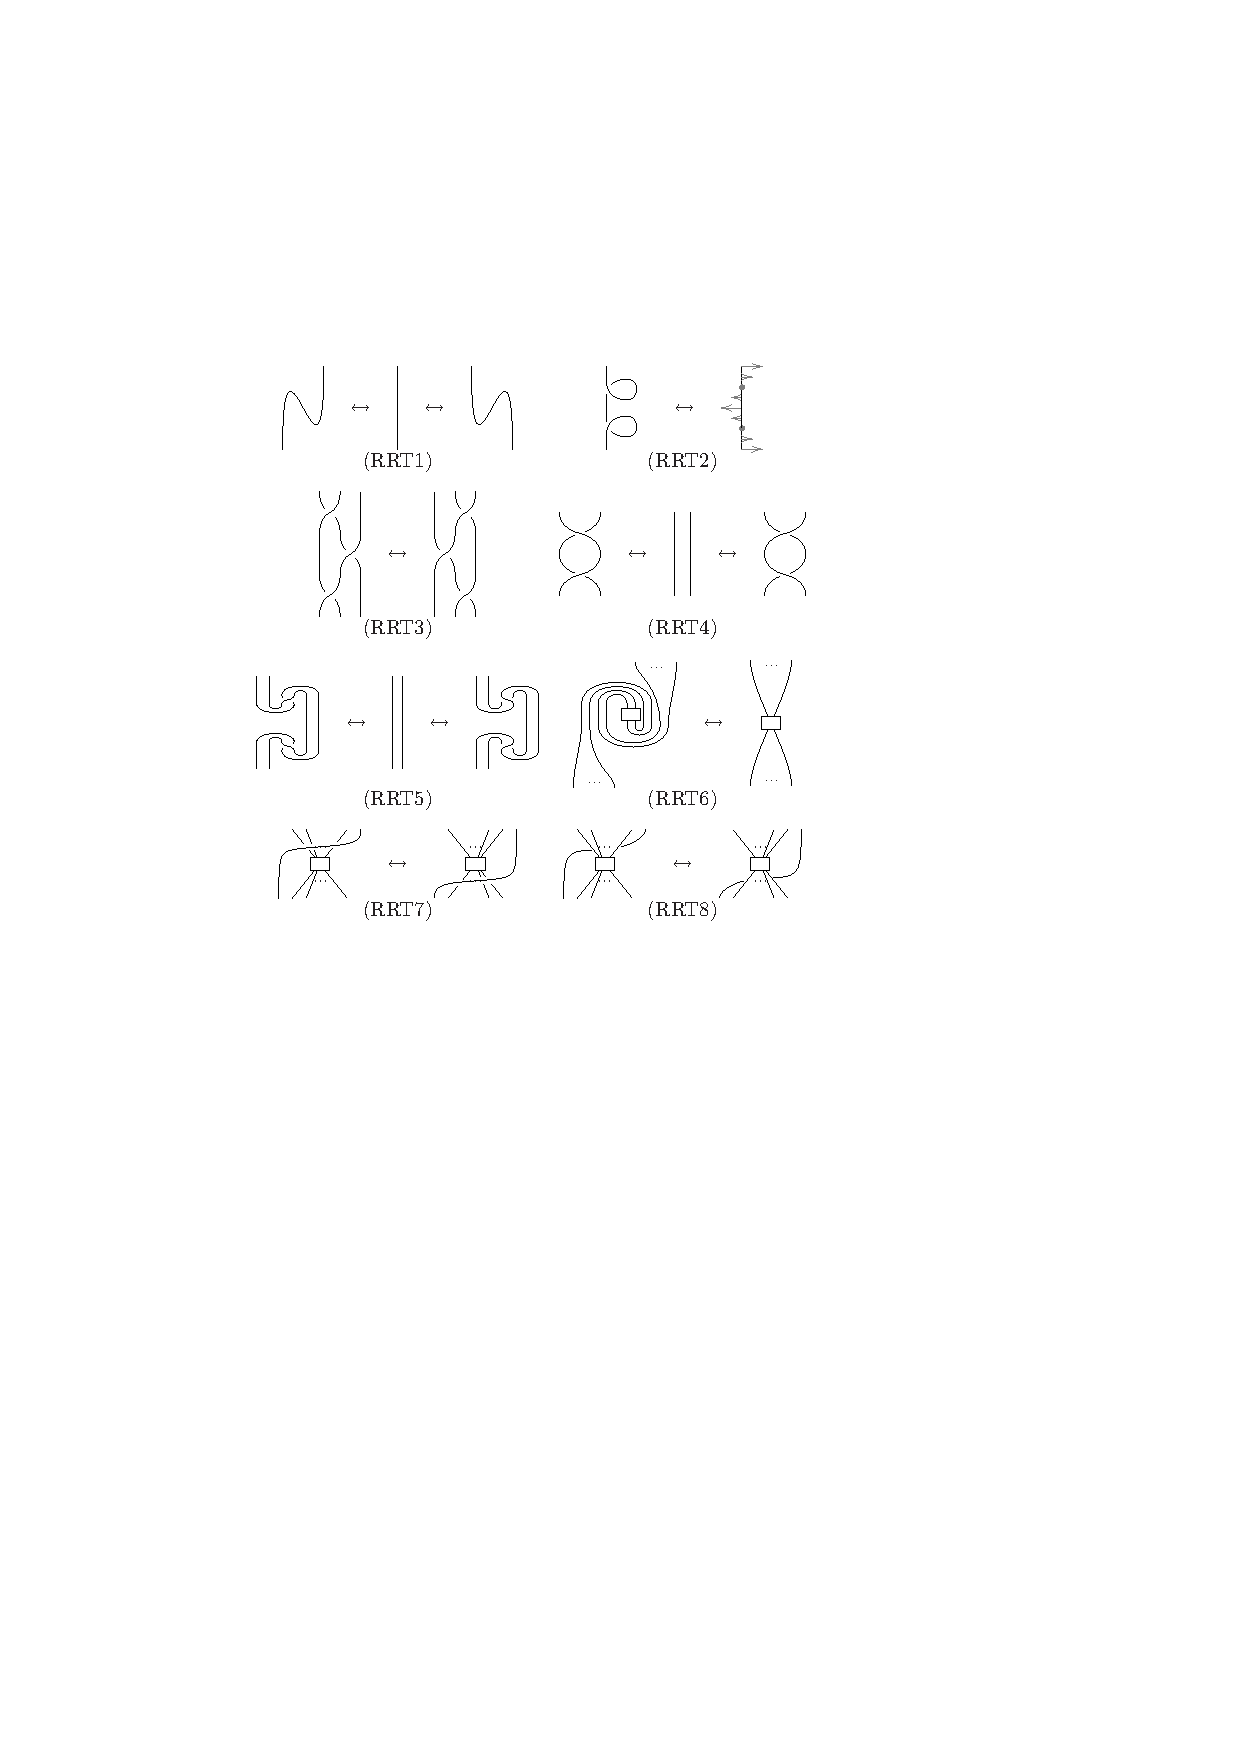
\includegraphics{fig-003}
  \caption{Reidmeister-Reshetikhin-Turaev moves for
    RT-diagrams. Note that move (RRT2) changes a trivial framing
    into a non-trivial (degree $1$) one.}
  \label{fig:gc-rrt}
\end{figure}

Let $\category{B}$ be a tensor category. A tensor functor
$\RTD[\A]\to{\category{B}}$ is uniquely specified if we define it on
the generators; it induces a tensor functor $\RTE[\A] \to \category{B}$
if it is compatible with relations (RRT1)--(RRT8).  In particular,
taking $\category{B}=\A$ we find the following (see also
\csref{thm:rt2} in \csref{cha:rt}).
\begin{theorem}[Reshetikhin-Turaev,
  \cite{reshetikhin-turaev;ribbon-graphs}]
  \label{thm:gc1}
  For any autonomous balanced braided tensor category $\A$, there is a
  tensor functor $Z_{\A}: \RTD[\A] \to \A$, mapping an object $(A_1,
  \ldots, A_r; \varepsilon_1, \ldots, \varepsilon_k) \in \RTD[\A]$ to $A_1^{\varepsilon_1} \otimes \dots \otimes
  A_k^{\varepsilon_k} \in \A$, and defined on generators of morphisms in
  $\RTD[\A]$ by
\begin{center}
  \everyxy={/r24pt/:}
  %% Figura 4
  {%
    \begin{tabular}{ccc}
      $\xy*!LC\xybox{%
        \vcross~{(0,1)*+{B}}{(1,1)*+{A}}{(0,0)*+{A}}{(1,0)*+{B}}}\endxy
      \mapsto \tau_{XY},$
      %\label{graph-cross+}
      &
      $\xy*!LC\xybox{%
        \vcross~{(0,0)*+{B}}{(1,0)*+{A}}{(0,1)*+{A}}{(1,1)*+{B}}}\endxy
      \mapsto \tau_{XY}^{-1},$
      %\label{graph-cross-}
      &
      $\xy*!LC\xybox{
        (0,1)*+[F]{f};%
        (-1,0)*+{A_1}**\dir{-},(-0.5,0)*+{A_2}**\dir{-},%
        (0,0.5)*+{\ldots},(1,0)*+{A_r}**\dir{-},%
        (-1,2)*+{B_1}**\dir{-},(-0.5,2)*+{B_2}**\dir{-},%
        (0,1.5)*+{\ldots},(1,2)*+{B_s}**\dir{-},%
        }\endxy \mapsto f$
      %\label{graph-morphism} 
      \\
      $\xy*!LC\xybox{%
        \vloop~{(0,1)}{(1,1)}{(0,0)*+{A}}{(1,0)*+{A}}}\endxy \mapsto
      \ev_{A},$
      %\label{graph-casimir}
      &
      $\xy*!LC\xybox{%
        \vloop~{(0,0)}{(1,0)}{(0,1)*+{A}}{(1,1)*+{A}}}\endxy \mapsto
      \coev_{A},$
      %\label{graph-coupling}
      &
      $\xy*!LC\xybox{(0,0)*+{A};(0,1)*+{A}**\dir{-}}\endxy \mapsto
      \id_X,$
      %\label{graph-id}
    \end{tabular}
    }
  \end{center}
where $\tau_{AB}$, $\ev_A$, $\coev_A$ are the structure maps in
$\A$, and $f$ is a morphism in $\A$; take the dual of an
object if the sign $\varepsilon$ on the corresponding edge is $-1$.

The tensor functor $Z_\A$ is invariant by the
Reidmeister-Reshetikhin-Turaev moves (RRT1)--(RRT8), so it induces a
tortile braided functor $Z_\A: \RTE[\A] \to \A$.
\end{theorem}
By definition of a symmetric category,
\begin{equation*}
  \tau_{AB} = \tau_{BA}\inv,
\end{equation*}
which imposes 
\begin{equation*}
  Z \left( 
    \xy*!LC\xybox{%
      \vcross~{(0,1)*+{B}}{(1,1)*+{A}}{(0,0)*+{A}}{(1,0)*+{B}}
      }\endxy \right)
  = 
  Z \left(
    \xy*!LC\xybox{%
      \vcross~{(0,0)*+{A}}{(1,0)*+{B}}{(0,1)*+{B}}{(1,1)*+{A}}
      }\endxy \right),
\end{equation*}
therefore we can quotient the set of morphisms of $\RTE[\A]$ by one
more relation
\begin{equation}
  \label{eq:S}\tag{S}
    \xy*!LC\xybox{%
      \vcross~{(0,1)*+{B}}{(1,1)*+{A}}{(0,0)*+{A}}{(1,0)*+{B}}
      }\endxy
  = 
    \xy*!LC\xybox{%
      \vcross~{(0,0)*+{A}}{(1,0)*+{B}}{(0,1)*+{B}}{(1,1)*+{A}}
      }\endxy.
\end{equation}
\begin{definition}
  The category $\RTG[\A]$ is the category whose set of morphisms is
  the quotient of $\Hom\RTE[\A]$ by the symmetry relation \eqref{eq:S}
  above. 

  The category $\RTG[\A]$ is monoidal braided autonomous and tortile
  with the structure maps induced from $\RTE[\A]$.
\end{definition}
Since $\Hom\RTE[\A]$ is the set of all isotopy classes of RT-graphs
embedded in 3-space, then $\Hom\RTG[\A]$ is the set of all (abstract)
$1$-dimensional CW-complexes equipped with the additional data
defining an $\A$-colored RT-graph, that is, for each edge $\ell$:
\begin{inparaenum}
\item an object $A_\ell \in \A$,
\item an orientation $\varepsilon_\ell$ of $\ell$,
\item a framing $N_\ell$,
and, finally, for each vertex $v$,
\item a morphism $f_v$ whose source and target match those of the
  vertex.
\end{inparaenum}

\begin{theorem}
\label{thm:gc2}
Let $\A$ be a tortile autonomous symmetric tensor category. Then
Reshetikhin-Turaev's graphical calculus induces a fully
faithful\footnote{With the proviso that one should always choose the
  inverses of the assignments in \csref{thm:gc1} for structure maps,
  e.g., for the braiding $\tau_{AB}$ one has to choose the
  representation as a ``crossing'' (see \textsl{(a)} below) and not
  the one as a ``vertex'' (see \textsl{(b)} below).
  \begin{center}
    \begin{tabular}{rlcrl}
      \textsl{(a)}
      &
      {\xyc
        \vcross~{(0,1)*+{B}}{(1,1)*+{A}}{(0,0)*+{A}}{(1,0)*+{B}}
        \endxyc}
      &
      % empty space
      &
      \textsl{(b)}
      &
      {\xyc 
        (0.5,0.5)*[F]{\scriptstyle \tau_{AB}}="o",%
        "o";(0,1)*{B}**\dir{-},%
        "o";(1,1)*{A}**\dir{-},%
        "o";(0,0)*{A}**\dir{-},%
        "o";(1,0)*{B}**\dir{-},%
        \endxyc}
    \end{tabular}
  \end{center}}
  braided tensor functor $Z_{\A}\colon\RTG[\A]\to\A$.
\end{theorem}
Since $Z_\A$ is a fully faithful functor, we can represent a morphism
in $\A$ by the associated RT-graph in $\RTG[\A]$; what is more, two
morphisms which are represented by isomorphic RT-graphs are equal.  By
definition of a tensor functor, the following relations hold:
\begin{gather*}
  Z_{\A}(\Gamma\circ\Phi) = Z_{\A}(\Gamma) \circ Z_{\A}(\Phi), 
  \qquad 
  Z_{\A}(\Gamma\otimes\Phi) = Z_{\A}(\Gamma) \otimes Z_{\A}(\Phi),
  \\
  Z_{\A}(a\Gamma + b\Phi) = aZ_{\A}(\Gamma) + bZ_{\A}(\Phi).
\end{gather*}
To make notation easier, we shall often suppress ``$Z_\A$'' from
displayed equations.


\section{Graphical calculus for ribbon graphs}
\label{sec:gc-ribbon-graphs}

We want now to define a variant of graphical calculus suitable for
application to ribbon graphs. Such graphs arise both in Feynman
expansions of Hermitian matrix integrals and in orbifold
cellularizations of moduli spaces of curves, which is one of the key
ideas in Kontsevich' proof of Witten's conjecture.

Any ribbon graph can be realized (in many different ways) as an
RT-graph. So, in order to define a graphical calculus on ribbon graphs
it suffices to define it on RT-graphs in a way that is independent of
the particular realization chosen.

\begin{definition}\label{dfn:ribbon-graphs}
  A \emph{ribbon graph} of type $(p,q)$ is a purely 1-dimensional
  CW-complex $\Gamma$ with 
  \begin{enumerate}
  \item $p+q$ endpoints divided into two ordered subsets $\In(\Gamma)$ and
    $\Out(\Gamma)$ with $\card{\In(\Gamma)}=p$ and $\card{\Out(\Gamma)}=q$;
  \item a cyclic order on half edges stemming from each vertex.
  \end{enumerate}
  The linear spans $\RG(p,q)$ of ribbon graphs of type $(p,q)$ define the
  $\Hom$-spaces of the category $\RG$ of ribbon graphs.
\end{definition}

Ribbon graphs arose in connection with a certain cellular
decomposition of the moduli space of smooth complex curves (see
\csref{sec:mgn-comb}). The connection is, very roughly, the following:
choose a ribbon graph $\Gamma$ of type $(0,0)$; one can use the cyclic
order to ``fatten'' edges into thin ribbons --- so we turn the graph
into a compact oriented surface with boundary $S(\Gamma)$.\FIXME{Tutto
  questo {\'e} spiegato pi{\'u} dettagliatamente a
  p.~\pageref{sec:mgn-comb}.  Meglio anticipare qui?}

Notice that this fattening procedure actually selects some homological
$1$-cycles in $\Gamma$, those corresponding to the boundary components
of $S(\Gamma)$. By abuse of language, we shall call these $1$-cycles
``boundary components'' or ``holes'', for short.

Denote $\Vertices{\Gamma}$, $\Edges{\Gamma}$ and $\Holes{\Gamma}$ the
sets of vertices, edges and holes of a graph $\Gamma$.

The number $n$ of boundary components and the genus $g$ of the ribbon
graph $\Gamma$ are defined to be those of the surface $S(\Gamma)$.
\begin{remark}
  Notice that the above construction, and the definitions of ``genus''
  and ``holes'' are meaningful only for ribbon graphs of type $(0,0)$.
\end{remark}

Recall that any vertex $v$ of a RT-graph has the set of incident edges
partitioned into disjoint totally ordered subsets $\In(v)$ and
$\Out(v)$.  There is a natural forgetful functor $\RTG\to\RG$ which
forgets orientations on edges and at each vertex $v$ remembers only
the cyclic order induced by the total order on $\In(v)$ and $\Out(v)$:
see \csref{fig:rt-to-cyclic}.
%% Figura 10
\begin{figure}
  \begin{equation*}
    {%
      \xy*!LC\xybox{
        (0,1)*+[F]{\ };%
        (-1,0)**\dir{-},(-0.5,0)**\dir{-},%
        (0,0.5)*+{\ldots},(1,0)**\dir{-},%
        (-1,2)**\dir{-},(-0.5,2)**\dir{-},%
        (0,1.5)*+{\ldots},(1,2)**\dir{-},%
        }\endxy\mapsto
      \xy*!LC\xybox{
        (0,1)*{\bullet};%
        (-1,0)**\dir{-},(-0.5,0)**\dir{-},%
        (0,0.5)*+{\ldots},(1,0)**\dir{-},%
        (-1,2)**\dir{-},(-0.5,2)**\dir{-},%
        (0,1.5)*+{\ldots},(1,2)**\dir{-},%
        ,(0,1.3);(0,1)%
        ,{\ellipse<>{-}},(0.02,1.3)*{\scriptscriptstyle{\langle}}
        }\endxy
      }
  \end{equation*}
  \caption{The cyclic order induced at a vertex of an RT-graph.}
  \label{fig:rt-to-cyclic}
\end{figure}
\begin{lemma}
  The set of ribbon graphs $\Hom\RG$ is the quotient of the set of
  RT-graphs $\Hom\RTG$ with respect to relations generated by the
  following moves
  \begin{enumerate}[(M1)]%\setcounter{enumi}{2}
  \item \label{M3} reverse orientation on edges;
  \item \label{M4} the first (resp. the last) edge in $\In(v)$ becomes the
    first (resp. the last) edge in $\Out(v)$ and vice-versa
    %% Figura 11
    \vspace*{4ex}
    \begin{equation*}
      {%
        \xy*!LC\xybox{
          (0,1)*+[F]{\ };%
          (-1,0)**\dir{.},(-0.5,0)**\dir{-},%
          (0,0.5)*+{\ldots},(1,0)**\dir{-},%
          (-1,2)**\dir{-},(-0.5,2)**\dir{-},%
          (0,1.5)*+{\ldots},(1,2)**\dir{-},%
          (-.45,1)*{\uparrow}
          }\endxy\quad,\quad\xy*!LC\xybox{
          (0,1)*+[F]{\ };%
          (-1,0)**\dir{-},(-0.5,0)**\dir{-},%
          (0,0.5)*+{\ldots},(1,0)**\dir{-},%
          (-1,2)**\dir{.},(-0.5,2)**\dir{-},%
          (0,1.5)*+{\ldots},(1,2)**\dir{-},%
          (-.45,1)*{\downarrow}
          }\endxy\quad,\quad
        \xy*!LC\xybox{
          (0,1)*+[F]{\ };%
          (-1,0)**\dir{-},(0.5,0)**\dir{-},%
          (0,0.5)*+{\ldots},(1,0)**\dir{.},%
          (-1,2)**\dir{-},(0.5,2)**\dir{-},%
          (0,1.5)*+{\ldots},(1,2)**\dir{-},%
          (.45,1)*{\uparrow}
          }\endxy\quad,\quad\xy*!LC\xybox{
          (0,1)*+[F]{\ };%
          (-1,0)**\dir{-},(0.5,0)**\dir{-},%
          (0,0.5)*+{\ldots},(1,0)**\dir{-},%
          (-1,2)**\dir{-},(0.5,2)**\dir{-},%
          (0,1.5)*+{\ldots},(1,2)**\dir{.},%
          (.45,1)*{\downarrow}
          }\endxy
        }
    \end{equation*}
  \end{enumerate}
\end{lemma} 

Let $V$ be a vector space over $\fk$ equipped with a symmetric inner
product $b\colon V\tp{2} \to \fk$. Construct the category $\btpc{V,b}$ (as
in \csref{sec:bosonic}); it is an autonomous tortile category and any
$V\tp{p}$ is a self-dual object.
\begin{definition}
  \label{dfn:rg-algebra}
  An $\RG$-agebra structure on $V$ is given by a tortile braided
  monoidal functor $F:\RG \to \freemc{V}$ which restricts to a
  bijection on the set of objects.
\end{definition}
More generally, one can define $\category{C}$-algebra structure, for
an arbitrary tortile braided tensor category $\category{C}$.

By definition, in any autonomous symmetric tensor category $\A$ there
are natural isomorphisms (see \csref{sec:duality})
\begin{equation*}\label{eq:passing-up-and-down}
  \A(X\otimes Y, Z) \longleftrightarrow \A(X, Z\otimes\rdl{Y}),
  \qquad
  \A(X\otimes Y, Z) \longleftrightarrow \A(Y, \ldl{X}\otimes Z),
\end{equation*}
for all $X, Y, Z \in \A$. For instance, the second bijection above maps
a morphism $f\colon X \otimes Y \to Z$ to the composition
\begin{equation*}
  X \xrightarrow{\coev_Y \otimes \id_X} \ldl{Y} \otimes Y \otimes X %
  \xrightarrow{\id_{\ldl{Y}} \otimes f} \rdl{Y} \otimes Z.%
\end{equation*}
In graphical notation, this reads:
%% Figura 12
\begin{equation*}
  {\xy*!LC\xybox{%
      (0,1)*+[F]{\rdl{f}};%
      (0,0)*{X}**\dir{-},%
      (-1,2)*{\rdl{Y}}**\dir{-},(1,2)*{Z}**\dir{-},%
      }\endxy
    \joinrel:=
    \xy*!LC\xybox{% 
      (0,1)*+[F]{f}="x";%
      (1,0)*{X}**\dir{-},%
      \vloop~{(-1,0.5)}{"x"+DL+/d6mm/}{(-1,2)}{"x"+DL+/r1mm/}|{Y},%
      (1,2)*{Z}**\dir{-},%
      }\endxy}
\end{equation*}
Within $\btpc{V,b}$, maps in \csref{eq:passing-up-and-down} translate
into linear isomorphisms:
\begin{gather}
  \Hom(V\tp{p}\otimes V\tp{q}, V\tp{r}) \longleftrightarrow \Hom(V\tp{p},
  V\tp{r}\otimes V\tp{q}),
  \label{eq:right-rot}
  \\
  \Hom(V\tp{p}\otimes V\tp{q}, V\tp{r}) \longleftrightarrow \Hom(V\tp{q},
  V\tp{p}\otimes V\tp{r}), 
  \label{eq:left-rot}
\end{gather}
for all $p,q,r \in \setZ$.

\begin{definition}\label{dfn:cyclic-algebra}
  A cyclic algebra structure on $(V, b)$ is a sequence
  $\{T_r\}_{r\in\setN}$ of cyclically invariant linear maps $T_r \colon
  V\tp{r} \to \fk$,:
  \begin{equation*}
    T_r (X_1 \otimes \dots \otimes X_{r-1} \otimes X_r) = 
    T_r (X_r \otimes X_1 \otimes \dots \otimes X_{r-1}).
  \end{equation*}
\end{definition}
Fix a cyclic algebra structure $\{T_r\}$ on $V$.  Each map $T_r$
in turn defines linear maps $T_{p,q}\colon V\tp{p} \to V\tp{q}$, for all
$p$ and $q$ such that $p+q=r$, via the isomorphisms
\csref{eq:right-rot} and \csref{eq:left-rot}; cyclical
invariance guarantees that $T_{p,q}$ does not depend on the
particular sequence of isomorphisms \csref{eq:right-rot} and
\csref{eq:left-rot}: any one yielding the right source and
target is good.

\begin{theorem}\label{thm:gc-cyc}
  Let $V$ be a vector space. Then the following data are equivalent:
  \begin{enumerate}
  \item cyclic algebra structures on $V$;
  \item $\RG$-algebra structures on $V$.
  \end{enumerate}
\end{theorem}
\begin{proof} Let $Z\colon\RG\to\btpc{V,b}$ be an $\RG$-algebra strcuture.
  Then
  \begin{align*}
    b &\joinrel:= Z\left(\xy*!LC\xybox{%
        \vloop~{(0,0.5)}{(1,0.5)}{(0,-0.5)}{(1,-0.5)},(0,-0.7)*{1^{\textrm{in}}}%
        ,(1,-0.7)*{2^{\textrm{in}}}}
      \endxy\right)
    \\
    T_r &\joinrel:= Z\left(\xy*!LC\xybox{
        (0,1)*{\bullet};%
        (-1,0)*+{1^{\textrm{in}}}**\dir{-},(-0.5,0)*+{2^{\textrm{in}}}**\dir{-},%
        (0,0.5)*+{\ldots},(1,0)*+{i^{\textrm{in}}}**\dir{-},%
        (-1,2)*+{r^{\textrm{in}}}**\dir{-}%
        ,(-0.5,2)*+{\ \ \ (r-1)^{\textrm{in}}}**\dir{-},%
        (0,1.5)*+{\ldots},(1,2)*+{(i+1)^{\textrm{in}}}**\dir{-},%
        }\endxy\right) 
  \end{align*}
  defines a cyclic algebra structure on $V$.
  
  Vice-versa, let $(V,b,T_1,T_2,\dots)$ be a cyclic algebra.  Pick any
  ribbon graph $\Gamma$ and realize it as an RT-graph; call this RT-graph
  $\hat\Gamma$. Give $\hat\Gamma$ the structure of a $\btpc{V,b}$-colored
  RT-graph by coloring edges of $\hat\Gamma$ with $V$ and vertices $v$
  with $T_{\card{\In(v)},\card{\Out(v)}}$. Denote the
  $\btpc{V,b}$-colored RT-graph obtained this way by $\hat\Gamma_V$. Two
  realizations of $\Gamma$ as an RT-graph differ by a finite sequence of
  moves M1, M2. Since $V$ is self-dual, the graphical calculus
  $Z_{\btpc{V,b}}(\hat\Gamma_V)$ is independent of the orientation on the
  edges, i.e., it is invariant with respect to the move M1. Moreover
  relations provided by \csref{thm:passing-up-and-down} give the
  invariance of $Z_{\btpc{V,b}}(\hat\Gamma_V)$ with respect to moves of
  type M2:
  \begin{equation*}
    %% Figura 13
    {%
      \xymatrix{
        \begin{xy}
          (0,0)*!LC\xybox{\rgvertex{10}%
            \loose2\missing3\loose4\loose5% sopra la riga
            \loose7\loose8\missing9\loose{10}},% sotto la riga
          (-0.5,0)*!LC{\ };(3,0)**\dir{.}
        \end{xy}
        \ar@{|->}[d] \ar@{=}[r]&      
        \begin{xy}
          (0,0)*!LC\xybox{\rgvertex{11}%
            \loose2\missing3\loose4,% sopra la riga
            (-1,1);"CENTER"**\crv{"AUXii6"+/d6pt/},% lato curvo sotto la
                                % riga 
            \loose7\loose8\missing{10}\loose{11}},% lati dritti sotto la
                                % riga
          (-1,0);(3.5,0)*!LC{\ }**\dir{.}
        \end{xy}
        \ar@{|->}[d]
        \\
        \xy*!LC\xybox{%
          (0,1)*+[F]{T_{p,q}};%
          (-1,0)**\dir{-},(-0.5,0)**\dir{-},(0,0.5)*{\ldots},(1,0)**\dir{-},%
          (-1,2)**\dir{-},(-0.5,2)**\dir{-},(0,1.5)*{\ldots},(1,2)**\dir{-},%
          }\endxy
        \ar@{=}[r]&
        \xy*!LC\xybox{% 
          (0,1)*+[F]{T_{p+1,q-1}}="x";%
          (-1,0)**\dir{-},(-0.5,0)**\dir{-},(0,0.5)*{\ldots},(1,0)**\dir{-},%
          \vloop~{(-1.2,0.9)}{"x"+DL+/d11pt/}{(-1.2,2)}{"x"+DL+/r6pt/},%
          (-0.5,2)**\dir{-},(0,1.5)*{\ldots},(1,2)**\dir{-},%
          }\endxy
        }
      }
  \end{equation*}
  Therefore, $Z(\Gamma)\joinrel:=Z_{\btpc{V,b}}(\hat\Gamma_V)$ is a well
  defined $\RG$-algebra structure on $V$.
\end{proof}
\begin{remark}
  The tensors $T_r$ are \emph{generators} of the $\RG$-algebra
  structure on $V$; as such, they are independent and need not satisfy
  any further compatibility relation. For instance, cyclic algebras
  need not be associative.
\end{remark}


\section{Graphical calculus for ordinary graphs}
\label{sec:graph-calc-graphs}

It is now easy to adapt constructions above to ordinary graphs. 
Note that a graph can be obtained from a ribbon graph by forgetting
the cyclic order on the edges incident to any vertex. Two ribbon
graphs leading to the same graph differ just by a permutation of the
edges incident to some vertices, so, to define a graphical calculus
for graphs, it will suffice to have a graphical calculus for ribbon
graphs, invariant with respect to the action of symmetric groups.

\begin{definition}
  \label{dfn:symmetric-algebra}
  A symmetric algebra structure on $(V, b)$ is a sequence
  $\{S_r\}$ of linear maps $S_r \colon V\tp{r} \to \fk$ such that
  \begin{equation*}
    S_r (X_1 \otimes \dots \otimes X_r) = S_r
    (X_{\sigma(1)} \otimes\dots \otimes X_{\sigma(r)}), 
    \quad \forall\sigma\in\Perm{r},
  \end{equation*}
  that is, maps $\{S_r\}$ are invariant with respect to the action of
  the symmetric group.
\end{definition}
Like in a cyclic algebra, the tensors $S_r$ are independent one from
the other: they should be regarded as generators of a tensor category
algebra structure.
\begin{definition}
  \label{dfn:symmetric-graph-category}
  Denote by $\SG$ the category whose morphisms are (ordinary
  topological) graphs: $\SG(p,q)$ is the linear span of graphs of type
  $(p,q)$. It is the quotient of $\RG$ by the action of symmetric
  groups on half-edges stemming from any vertex.
\end{definition}  
\begin{definition}
  \label{dfn:sg-algebra}
  An $\SG$-agebra structure on $V$ is given by a tortile braided
  monoidal functor $F:\SG \to \freemc{V}$ which restricts to a
  bijection on the set of objects.
\end{definition}

\begin{theorem}\label{thm:gc-sym}
  Let $V$ be a vector space. Then the following data are equivalent:
  \begin{enumerate}
  \item symmetric algebra structures on $V$;
  \item $\SG$-algebra structures on $V$.
  \end{enumerate}
\end{theorem}
\begin{proof}
  A functor $Z\colon\SG\to\btpc{V,b}$ endows $V$ with a symmetric algebra
  structure, as in the proof of \csref{thm:gccyc}.
  
  Conversely, assume we are given a cyclic algebra structure on $V$.
  Since the tensors $S_r$ are symmetric, they are, in particular,
  cyclically invariant: so $(V,b,S_1,S_2,\dots)$ is a cyclic algebra
  and a braided functor $Z\colon\RG\to\btpc{V,b}$ is defined.  Since the
  tensors $\{S_k\}$ are symmetric, it factors through a braided
  tortile functor $Z\colon\SG\to\btpc{V,b}$.
\end{proof}
\begin{remark}
  \label{rem:many-sorted-graphs}
  So far, we have considered cyclic (resp. symmetric) algebras with
  only one $r$-ary operation for any $r\in\setN$. The graphical calculus
  formalism immediately generalizes to cyclic (resp. symmetric)
  algebras with a family of cyclic tensors $\{T_{r,\alpha}\}_{\alpha\in
    I_r}$
  (resp. a family of symmetric tensors $\{S_{r,\alpha}\}_{\alpha\in
    I_r}$);
  in fact, we only ought to consider graphs whose $r$-valent vertices
  are decorated with labels from $I_r$.

  The \emph{dual graphs} of stable curves \cite{deligne-mumford} provide
  an example --- they are ordinary graphs, with each vertex $v$
  decorated by an integer $g(v)$: it is the genus of an irreducible
  component of the algebraic curve corresponding to the graph. Such
  graphs were called \emph{modular graphs} in \cite{getzler-kapranov}.
\end{remark}

\section{A sample computation}
Let $(V,b,S_1,S_2,\dots)$ be a symmetric algebra. We want to compute
the operator
\begin{equation*}
  Z(\Gamma)\joinrel:=Z\left(
    \xy
    \rghole{3}\loose{1}\loose{2}\loose{3},(0,2)*{1^{\text{in}}}%
    ,(1.73,-1)*{2^{\text{in}}},(-1.73,-1)*{3^{\text{in}}}
    \endxy
  \right)\colon V^{\otimes 3}\to\fk
\end{equation*}
A realization of the graph $\Gamma$ as an RT-diagram is obtained by
hanging it by the vertices:
\begin{equation*}
  %% Figura 14
  {\xy*!LC\xybox{
      (-1,1)="a",(0,1)="b",(1,1)="c",(-0.4,-0.15)="buno",(-0.65,-0.2)="bdue",%
      (-1,-1)="d",(-.33,-1)="e",(1,-1)="f",%
      "a"*+[F]{S_3};"d"**\dir{-}?(.5)*\dir{<},%
      "c"*+[F]{S_3};"f"**\dir{-}?(.5)*\dir{<},%
      "b"*+[F]{S_3};"buno"**\crv{(0.15,0.1)},%
      "bdue";"e"**\crv{(-1.1,-0.27)&(-0.33,-0.9)}?(.5)*\dir{<},%
      "a"*+[F]{S_3};"b"*+[F]{S_3}**\crv{(-.5,-.5)}?(.8)*\dir{>},%
      "a"*+[F]{S_3};"c"*+[F]{S_3}**\crv{(0,-2.3)}?(.2)*\dir{>},%
      "b"*+[F]{S_3};"c"*+[F]{S_3}**\crv{(0.5,-.5)}?(.3)*\dir{>},%
      (-2.5,2);(2.5,2)**\dir{-},(-2.5,-1);(2.5,-1)**\dir{-}
      }\endxy}
\end{equation*}
Splitting the RT-diagram above into elementary pieces and applying
Reshetikhin-Turaev rules we find
\begin{align*}%
  Z(\Gamma)&=Z\left(\quad{\xy*!LC\xybox{
        (-1,1)="a",(0,1)="b",(1,1)="c",%
        (-0.4,-0.15)="buno",(-0.65,-0.2)="bdue",%
        (-1,-1)="d",(-0.33,-1)="e",(1,-1)="f",%
        "a"*+[F]{S_3};"d"**\dir{-}?(.5)*\dir{<},%
        "c"*+[F]{S_3};"f"**\dir{-}?(.5)*\dir{<},%
        "b"*+[F]{S_3};"buno"**\crv{(0.15,0.1)},% 
        "bdue";"e"**\crv{(-1.1,-0.27)&(-0.33,-0.9)}?(.5)*\dir{<},%
        "a"*+[F]{S_3};"b"*+[F]{S_3}**\crv{(-.5,-.5)}?(.8)*\dir{>},%
        "a"*+[F]{S_3};"c"*+[F]{S_3}**\crv{(0,-2.3)}?(.2)*\dir{>},% 
        "b"*+[F]{S_3};"c"*+[F]{S_3}**\crv{(0.5,-.5)}?(.3)*\dir{>},%
        (-2.5,2);(2.5,2)**\dir{-},(-2.5,-1);(2.5,-1)**\dir{-},
        (-1.6,0.35);(1.6,0.35)**\dir{.},%
        (-1.6,0.2);(1.6,0.2)**\dir{.},%
        (-1.6,-0.4);(1.6,-0.4)**\dir{.},%
        (-1.6,-0.75);(1.6,-0.75)**\dir{.},%
        (-1.6,2);(-1.6,-1)**\dir{.},%
        (1.6,2);(1.6,-1)**\dir{.},%
        (-0.5,2);(-0.5,0.35)**\dir{.},%
        (0.5,2);(0.5,0.35)**\dir{.},%
        (-0.1,0.35);(-0.1,0.2)**\dir{.},%
        (0.1,0.35);(0.1,-0.4)**\dir{.},%
        (-0.9,0.8);(-0.9,-1)**\dir{.},%
        (0.9,0.8);(0.9,-1)**\dir{.},%
        (-0.6,0.35);(-0.6,0.2)**\dir{.},%
        (0.6,0.35);(0.6,0.2)**\dir{.},%
        (-0.4,-0.47);(-0.47,-0.75)**\dir{.}}%
      \endxy}\quad\right)=\\&\\
  &\qquad=(S_3\otimes S_3\otimes S_3) \circ(\Id_V\otimes\Id_V\otimes\coev_V\otimes\Id_V\otimes\coev_V\otimes
  \Id_V\otimes\Id_V)\circ\\
  &\qquad\qquad(\Id_V\otimes\tau_{VV}^{}\otimes\Id_V\otimes\Id_V)\circ
  (\Id_V\otimes\Id_V\otimes\coev_V\otimes\Id_V)
\end{align*}%
If $\{e_i\}$ is a basis of $V$ and $\{e^i\}$ denotes the dual
basis with respect to the pairing $b$, then structure constants of
the symmetric algebra $(V,b,S_1,S_2,\dots)$ are
\begin{equation*}
  g_{ij}=b(e_i,e_j),\qquad g^{ij}\joinrel:=b(e^i,e^j),
\end{equation*}
\begin{equation*}
  (S_k)_{i_1,\dots,i_s}^{j_{s+1},\dots,j_k}\joinrel:=S_k(e_1\otimes\cdots\otimes
  e_{i_s}\otimes e^{j_{s+1}}\otimes\cdots\otimes e^{j_k}).
\end{equation*}
With these notations
\begin{equation*}
  \coev_V=\sum_{i,j}g^{ij}e_i\otimes e_j,
\end{equation*}
and the operator $Z(\Gamma)$ acts on basis elements by
\begin{equation*}
  Z(\Gamma)(e_\alpha\otimes e_\beta\otimes
  e_\gamma)=\sum_{\delta,\epsilon,\zeta,\eta,\vartheta,\iota}g^{\delta\epsilon}
  g^{\zeta\eta}g^{\vartheta\iota} (S_3)_{\alpha\delta\zeta}
  (S_3)_{\eta\beta\vartheta} (S_3)_{\iota\epsilon\gamma}.
\end{equation*}



%%% Local Variables: 
%%% mode: latex
%%% TeX-master: "index"
%%% End: 

\RCSID $Id: fd.tex,v 1.1 2002/01/10 10:01:51 ri Exp $
%auto-ignore


\chapter{Gaussian integrals and Feynman diagrams}
\label{sec:fd}
\everyxy={0,<2em,0em>:,(0,0.5),} % scala per i diagrammi

In this chapter is devoted to showing how a Gaussian integral can be
expanded into a sum of Feynman diagrams, within the framework of the
graphical calculus on symmetric categories.  Depending on the nature
of the integral, this formula will hold as a strict equality or in the
sense of asymptotic expansions. In particle physics, Gaussian
integrals and their Feynman diagrams expansions are used to describe
bosonic statistics.

The first description of Feynman diagrams via Graphical Calculus is
apparently due to R.~Oeckl \cite{oeckl;braided-qft}; the exposition
here, however, comes from joint work with D.~Fiorenza
\cite{murri-fiorenza;feynman}. 


\section{Gaussian measures and the Wick's lemma} 

Let \(V\) be a finite dimensional Euclidean space,
with inner product \(\inner{-}{-}\). If \(\{e_i\}\) is a basis of
\(V\), we denote the \emph{coordinate} maps relative to this basis as
\(e^i\colon V\to\setR\), and write \(v^i\) for the pairing
\(\pairing{e^i}{v}\).  The matrix associated to \(\inner{-}{-}\) with
respect to the basis \(\{e_i\}\) is given by
\begin{equation*}
  g_{ij} \joinrel:= \inner{e_i}{e_j}.
\end{equation*}
As customary, we set \(g^{ij} \joinrel:= (g^{-1})_{ij} = \inner{e^i}{e^j}\).

Let now \(\ud v\) be a (non trivial) translation invariant measure on
\(V\). The function \(\E^{-\onehalf\inner{v}{v}}\) is positive and
integrable with respect to \(\ud v\).
\begin{definition}\label{dfn:gaussian-measure}
  The probability measure on \(V\) defined by
  \begin{equation*}
    \ud\mu(v) \joinrel:= \frac{1}{C} \E^{-\onehalf\inner{v}{v}} \ud v, 
    \qquad
    C := {\int_V \E^{-\onehalf\inner{v}{v}} \ud v},
  \end{equation*}
  is called the \emph{Gaussian measure} on \(V\).
\end{definition}
Since a non-trivial translation invariant measure on \(V\) is unique up
to a scalar factor, \(\ud\mu\) is actually independent of the chosen
\(\ud v\).

The symbol \(\avg{f}\) denotes the \emph{average} of a function \(f\)
with respect to the Gaussian measure, i.e.,
\begin{equation*}
  \avg{f} \joinrel:= \int_V f(v)\ud\mu(v).
\end{equation*}

\begin{lemma}[Wick]
  Polynomial functions of the coordinates \(v^i\) are integrable with
  respect to \(\ud\mu\) and:
  \begin{align}
    \tag{W1}
    \avg{v^{i_1}v^{i_2}\cdots
      v^{i_{2n+1}}} &= 0,
    \\
    \tag{W2}
    \avg{v^{i}v^{j}} &= g^{ij},
    \\
    \tag{W3}
    \avg{v^{i_1}v^{i_2}\cdots
      v^{i_{2n}}} &= \sum\limits_{s\in P}
    g^{i_{s_1} i_{s_2}} g^{i_{s_3} i_{s_4}} \cdots
    g^{i_{s_{2n-1}} i_{s_{2n}}}, 
  \end{align}
  where the sum ranges over all distinct pairings of the set of
  indices \(\{i_1,\dots,i_{2n}\}\), i.e., over the set of all
  partitions \(\{\{i_{s_1},i_{s_2}\},\{i_{s_3},i_{s_4}\},\dots\}\) of
  \(\{i_1,i_2,\dots,i_{2n}\}\) into 2-element subsets.
\end{lemma}
For a proof of Wick's lemma see, for instance,
\cite{bessis-itzykson-zuber;graphical-enumeration}.

The inner product \(\inner{-}{-}\) extends uniquely to a Hermitian
product on the complex vector space \(\cplx{V} \joinrel:= V \otimes \setC\).
Identify \(V\) with the subspace \(V \otimes \{1\}\) of real vectors in
\(\cplx{V}\); \(\{ e_i \}\) is a real basis for the complex vector
space \(\cplx{V}\). Extend \(\avg{-}\) to tensor powers of real
vectors by
\begin{equation*}
  \label{eq:avg-x}
  \avg{v\tp{k}} \joinrel:= \sum \avg{v^{i_1} \cdot \cdots \cdot v^{i_k}}
  e_{i_1} \otimes \cdots \otimes e_{i_k},
\end{equation*}
so Wick's lemma can be recast this way:
\begin{align}
  \label{eq:W1}\tag{W1'}
  \avg{v\tp{ 2n+1}} &= 0,
  \\
  \label{eq:W2}\tag{W2'}
  \avg{v\tp{ 2}} &= \sum_{i,j} g^{ij} e_i
  \otimes e_j,
  \\
  \label{eq:W3}\tag{W3'}
  \avg{v\tp{2n}} &= \sum\limits_{i_1, \dots,
    i_{2n}} \sum\limits_{s\in P} g^{i_{s_1} i_{s_2}} \cdots
  g^{i_{s_{2n-1}} i_{s_{2n}}} e_{i_1} \otimes e_{i_2} \otimes \cdots
  \otimes e_{i_{2n-1}} \otimes e_{i_{2n}},
\end{align}
where the last sum ranges over all distinct pairings of indices in the
set \(\{i_1, \dots, i_{2n}\}\).


\section{From Wick's lemma to Feynman diagrams}
\label{sec:wick-to-fd}

The right-hand side of (\ref{eq:W2}) is the Casimir element
$\gamma_{\cplx{V}}$ of \(\{\cplx{V}, \inner{-}{-}\}\); in
Reshetikhin-Turaev's graphical notation, we can rewrite
\eqref{eq:W2} as
\begin{equation*}
  \avg{v\otimes v}= {\xy\vloop-\endxy}\ .
\end{equation*}
The graphical notation becomes particularly suggestive 
(and useful) when applied to \eqref{eq:W3}:
\begin{equation}
  \label{eq:avg-to-casimir}
  \begin{split}
    \avg{v\tp{ 4}} &=
    {%
      {\xy\vloop-,(1.2,0.5),\vloop-\endxy} +
      {\xy\vloop-|(.7)\knothole,(0.5,0.5),\vloop-\endxy} + 
      {\xy\vloop-,(0.7,0):(0.2,0.7),\vloop-\endxy}
    }\quad, \\
    \ldots& \\
    \avg{v\tp{ 2n}} &=
    {%
      \left({\xy\vloop-,(1.2,0.5),\vloop-,(1.2,0)\endxy} \cdots
        {\xy\vloop-\endxy}\right) +
      \dots +
      {\xy\vloop-,(0.7,0):(0.2,0.7),%
        \vloop-,(0.7,0.2)*\txt{\vdots},(0.24,0):(2.4,2.9)\vloop-\endxy}
      }\quad,
  \end{split}
\end{equation}
the last sum ranging over all possible configurations of \(n\) Casimir
elements and the braiding being the trivial one: \(x\otimes y\mapsto
y\otimes x\).  

In addition, assume we have, for any \(k\), a cyclically invariant
\(k\)-tensor
\begin{equation*}
  T_{k}:\cplx{V}{}\tp{k} \to \setC;
\end{equation*}
which has the graphical representation
\begin{equation*}
  \underbrace{\xy(0.3333,0):
    (0,0)="a",
    (2,0)="b",
    (4,0)="c",
    (6,0)="d",
    (3,4)="v",
    (3,5)="w",
    "v";"a"**\dir{-},
    "v";"b"**\dir{-},
    "v";"d"**\dir{-},
    "c"*\txt{\ldots},
    "w"*\txt{\(T_{k}\)},
    "v"*{\bullet}
    \endxy}_{k}
\end{equation*}

The data \((V, \inner{-}{-}, T_1, T_2, \dots)\) define a cyclic
algebra structure, so we can use Reshetikhin-Turaev's graphical
calculus \(\Gamma\mapsto Z(\Gamma)\) to compute averages
\begin{equation*}
  \bigl\langle T_1(v)^{l_1} T_2(v\tp{ 2})^{l_2} \cdots
  T_{k}(v\tp{ k})^{l_k} \bigr\rangle.
\end{equation*}
\begin{lemma}\label{thm:feynman-avg-gc}
  Any average \(\bigl\langle T_1(v)^{l_1} T_2(v\tp{ 2})^{l_2}
  \cdots T_{k}(v\tp{ k})^{l_k} \bigr\rangle\) is a linear
  combination \(\sum \alpha_\Gamma Z(\Gamma)\) where \(\Gamma\) runs
  in the set of ribbon graphs of type (0,0) with \(l_i\) vertices of
valence \(i\), for \(i=1,\dots,k\).
\end{lemma}
\begin{proof}
  By linearity of the \(T_k\)'s and \eqref{eq:avg-x},
  \begin{equation*}
    \avg{T_1(v)^{l_1} \cdots T_{k}(v\tp{ k})^{l_k}} = 
    \bigl(T_1\tp{l_1} \otimes \cdots \otimes T_{k}\tp{l_k} \bigr)
    \avg{v\tp{\sum_i il_i}}.
  \end{equation*}
  If \(\sum il_i\) is odd, \(\avg{v\tp{\sum il_i}}\) is zero, and the set
  of graphs considered in the statement is empty. If \(\sum il_i\) is
  even, according to graphical calculus rules, $\bigotimes_{i=1}^k
  T_i\tp{l_i}$ corresponds to the juxtaposition of $l_1$ univalent
  vertices, $l_2$ bivalent vertices, etc., up to $l_k$ vertices of
  valence $k$. In this case, \eqref{eq:avg-to-casimir} translates
  $\avg{v\tp{\sum il_i}}$ into edges connecting these vertices in all
  possible ways.
\end{proof}

\begin{example}
  For example,
  \begin{align*}
    \avg{\left(T_2(v\tp{ 2})\right)^2} &= 
    {%
      {\xy*!UC\xybox{
          /r 1cm/:
          ,(1,1.2);(1,1.2)**\crv{(0,0)&(2,0)},(1,1.2)*{\bullet}
          ,(1.8,1.2);(1.8,1.2)**\crv{(0.8,0)&(2.8,0)},(1.8,1.2)*{\bullet}
          }\endxy}
      + 2 \cdot 
      {\xy*!UC\xybox{
          /r 1cm/:
          ,(1,1.2);(1.8,1.2)**\crv{(0,0)&(2.8,0)},(1,1.2)*{\bullet}
          ,(1,1.2);(1.8,1.2)**\crv{(1.2,0.5)&(1.6,0.5)},(1.8,1.2)*{\bullet}
          }\endxy}
      }
    \\
    \avg{T_4(v\tp{ 4})} &=
    {%
      {\xy*!UC\xybox{
          /r 1cm/:
          ,(1,1.2);(1,1.2)**\crv{(-0.2,0)&(1.6,0)},(1,1.2)*{\bullet}
          ,(1,1.2);(1.05,.35)**\crv{(1,1.2)&(1.5,0.7)&(1.5,0.2)&(1.05,.35)}
          ,(1,1.2);(0.95,.45)**\crv{(1,1.2)&(0.8,0.5)&(0.95,.45)}
          }\endxy}
      + 2\cdot
      {\xy*!UC\xybox{
          /r 1cm/:
          ,(1,1.2);(1,1.2)**\crv{(-.4,0)&(.95,0)}
          ,(1,1.2);(1,1.2)**\crv{(1.05,0)&(2.4,0)}
          ,(1,1.2)*{\bullet}
          }\endxy}
      }
  \end{align*}
\end{example}

\begin{lemma}\label{thm:feynman-avg-coeff}
  The coefficient \(\alpha_\Gamma\) appearing in
  \csref{thm:feynman-avg-gc} is an integer given by:
  \begin{equation*}
    \alpha_\Gamma =
    \frac{1^{l_1} l_1! 2^{l_2} l_2! \cdots k^{l_k} l_k!}
    {\card{\Aut\Gamma}}.
  \end{equation*}
\end{lemma}
\begin{proof}
  Let \(X\) be the set of all ribbon graphs obtained by:
  \begin{inparaenum}
  \item juxtaposing \(l_1\) vertices of valence \(1\), \(l_2\)
    vertices of valence \(2\), etc., up to \(l_k\) vertices of valence
    \(k\), and,
  \item connecting them in all possible ways by means of arcs.
  \end{inparaenum}
  The constant \(\alpha_\Gamma\) counts the number of occurrences of graphs
  isomorphic to \(\Gamma\) in the set \(X\).
  
  The semi-direct product \(K = \prod_{i=1}^k(\Perm{l_i} \rtimes
(\setZ/i\setZ)^{l_i})\)
  acts on \(X\) as follows: the image of a graph
  \(\Phi\) is obtained by permuting vertices of the same valence and
  rotating edges incident to each vertex. Since this action is
  transitive on isomorphism classes,
  \begin{equation*}
    \alpha_\Gamma = \frac {\card{K}} {\card{\Stab_K(\Gamma)}}
    = \frac {\card{K}} {\card{\Aut\Gamma}}
    = \frac{1^{l_1} l_1! 2^{l_2} l_2! \cdots
      k^{l_k} l_k!}{\card{\Aut\Gamma}},
  \end{equation*}
  where $\Stab_K(\Gamma)$ is the stabilizer of $\Gamma$ under the
  action of $K$.
\end{proof}

\begin{theorem}[Feynman-Reshetikhin-Turaev]\label{thm:FRT}
  Let \(Z_{x_*}\) be the graphical calculus for the cyclic algebra
  \(A(x_*) \joinrel:= (V_{\setC}, \inner{-}{-}, x_1T_1, x_2T_2, \dots)\), where
  $x_1,x_2,\dots$ are complex variables. Then, the following
  asymptotic expansion holds:
  \begin{equation}
    \label{eq:FRT1}
    Z(x_*)\joinrel:=\int_V \exp \biggl\{ \sum_{k=1}^\infty x_k
    \frac{T_k(v\tp{k})}{k}
    \biggr\} \ud\mu(v) 
    = \sum_{\Gamma\in\RG(0,0)} \frac {Z_{x_*}(\Gamma)} {\card{\Aut\Gamma}},
  \end{equation}
  where the sum on the right ranges over the set $\RG(0,0)$ of all
  isomorphism classes of (possibly disconnected) ribbon graphs of type
  (0,0). The formal series $Z(x_*)$ is called the \emph{partition
    function} of the algebra $A(x_*)$.
\end{theorem}
\begin{proof}
  Expand in Taylor series the left-hand side:
  \begin{align*}
    \int_V \exp \biggl\{\sum_{k=1}^\infty &\frac{x_k}{k}T_k(v\tp{k})\biggr\}
    \ud\mu(v)=
    \\
    &= \sum_{n=0}^\infty \sum_{\nu_1, \dots, \nu_n} \frac{x_{\nu_1} \dots
      x_{\nu_n}} {n!\nu_1 \cdots \nu_n} \avg{T_{\nu_1}(v\tp{ \nu_1}) \cdots
      T_{\nu_n}(v\tp{\nu_n})}
    \\
    &= \sum_{k=0}^\infty \sum_{l_1, \dots, l_k} \frac{x_1^{l_1} \cdots x_k^{l_k}}
    {1^{l_1} l_1! 2^{l_2} l_2! \cdots k^{l_k} l_k!}  \avg{T_{1}(v)^{l_1}
      \cdots T_{k}(v\tp{k})^{l_k}}
    \\
    &= \sum_{k=0}^\infty \sum_{l_1, \dots, l_k} \frac
    {\avg{\bigl(x_1T_{1}(v)\bigr)^{l_1} \cdots
        \bigl(x_kT_{k}(v\tp{k})\bigr)^{l_k}}} {1^{l_1} l_1! 2^{l_2}
      l_2! \cdots k^{l_k} l_k!}, 
    \\
    &= \sum_{\Gamma \in \RG(0,0)} \frac{Z_{x_*} (\Gamma)}
{\card{\Aut\Gamma}},
  \end{align*}
  by lemmas~\ref{thm:feynman-avg-gc} and~\ref{thm:feynman-avg-coeff}.
\end{proof}
A similar argument yields:
\begin{equation}
  \label{eq:FRT2}
  \int_V \frac{T_1(v)^{l_1} T_2(v\tp{2})^{l_2} \cdots
    T_k(v\tp{k})^{l_k}} {1^{l_1} l_1! 2^{l_2} l_2! \cdots k^{l_k}
    l_k!} \exp \left\{ \sum_{k=1}^\infty x_k\frac{T_k(v\tp{k})}{k}
    \right\} \ud\mu(v)
    = \sum_{\Gamma} \frac{Z_{x_*}(\Gamma)}{\card{\Aut\Gamma}}
\end{equation}
where the sum in the right-hand side ranges over all ribbon graphs
having $l_i$ ``special'' \(i\)-valent vertices (for $i=1\dots,k$), and
$\Aut(\Gamma)$ is the group of automorphisms that map the set of special
vertices to itself. In \eqref{eq:FRT2}, the graphical calculus
$Z_{x_*}$ interprets each $i$-valent special vertex as the operator
$T_i$ and each ordinary $i$-valent vertex as the operator $x_iT_i$.
This is the same as considering graphs with two sorts of vertices (see
\csref{rem:many-sorted-graphs}), one decorated by operators $T_i$
(call them ``special vertices''), and the other decorated by $x_iT_i$
(call them ``ordinary'').

%\begin{rem} Notice that we can recast the cyclical invariance of the
%  tensors \(T_k\) by saying \(\Aut(T_k)=\setZ/k\setZ\). The statement of
%  \csref{thm:FRT} can be rewritten as
%\begin{equation}\label{eq:FRTeqbis}
%    \int_V \exp \biggl\{ \sum_{k=1}^\infty x_k
%\frac{T_k(v\tp{k})}{\card{\Aut(T_k)}}
%    \biggr\} \ud\mu(v)
%    = \sum_{\Gamma} \frac {Z_{x_*}(\Gamma)} {\card{\Aut\Gamma}},
%\end{equation}
%while equation \eqref{eq:FRT2} becomes
%\begin{equation}
%  \label{eq:feynmanturaevduebis}
%  \int_V \frac{T_1(v)^{l_1} T_2(v\tp{2})^{l_2} \cdots
%    T_k(v\tp{k})^{l_k}} {\card{\Aut(T_1^{\otimes l_1}\otimes
%T_2^{\otimes l_2}
%\cdots \otimes T_k^{\otimes l_k})}} \exp \left\{ \sum_{k=1}^\infty
%x_k\frac{T_k(v\tp{k})}{\card{\Aut(T_k)}}
%    \right\} \ud\mu(v)
%    = \sum_{\Gamma} \frac{Z_{x_*}(\Gamma)}{\card{\Aut\Gamma}},
%\end{equation}
%where the last sum ranges over graphs having $l_1$ distinguished
%$1$-valent vertices, $l_2$ $2$-valent ones, etc.
%\end{rem}

\csref{thm:FRT} can be straightforwardly adapted to a symmetric
algebra \((V, \inner{-}{-},\break S_1, S_2, \dots)\).
\begin{theorem}[Feynman-Reshetikhin-Turaev]\label{thm:FRTsym}
  Let \(Z_{x_*}\) be the graphical calculus for the symmetric algebra
  \((V_{\setC}, \inner{-}{-}, x_1S_1, x_2S_2, \dots)\), where
$x_1,x_2,\dots$ are
  complex variables. The following asymptotic expansion holds:
  \begin{equation*}
    Z(x_*)\joinrel:=\int_V \exp \biggl\{ \sum_{k=1}^\infty x_k
    \frac{S_k(v\tp{k})}{k!}
    \biggr\} \ud\mu(v)
    = \sum_{\Gamma\in\SG(0,0)} \frac {Z_{x_*}(\Gamma)} {\card{\Aut\Gamma}},
  \end{equation*}
  where the sum on the right ranges over all isomorphism classes of
(possibly disconnected) ordinary graphs of type (0,0).
\end{theorem}

\begin{example} 
  Let \(\phi\) be an analytic function defined in the whole \(V\). The
  Taylor expansion formula
\begin{equation*}
\phi(v)=\phi(0)+\sum_{n=1}^{\infty}\frac{D^n\phi\vert_0(v^{\otimes
n})}{n!},
\end{equation*}
together with \csref{thm:FRTsym}  gives
\begin{equation}
  \int_V \E^{\phi(v)} \ud
  \mu(v) = \E^{\phi(0)} \cdot \left(\sum_\Gamma
    \left.\frac{D_\Gamma(\phi)}{\card{\Aut\Gamma}}\right\vert_0\right).
\end{equation}
\end{example}

%\begin{rem} Since the tensors \(S_k\) are symmetric,
%  \(\Aut(S_k)=\Perm{k}\), so we can write the analogues of formulas
%  \eqref{eq:FRTeqbis} and \eqref{eq:feynmanturaevduebis}:
%  \begin{gather}
%    \label{eq:FRTsymeqbis}
%    \int_V \exp \biggl\{ \sum_{k=1}^\infty x_k
%    \frac{S_k(v\tp{k})}{\card{\Aut(S_k)}}   
%    \biggr\} \ud\mu(v)
%    = \sum_{\Gamma} \frac {Z_{x_*}(\Gamma)} {\card{\Aut\Gamma}},
%    \\
%    \label{eq:feynmanturaevsymbis}
%        \int_V \frac{S_1(v)^{l_1} 
%%          S_2(v\tp{2})^{l_2} 
%          \cdots
%          S_k(v\tp{k})^{l_k}} {\card{\Aut(S_1\tp{l_1}\otimes 
%%            S_2\tp{l_2}
%            \cdots \otimes S_k\tp{l_k})}}
%        \exp \left\{ 
%          \sum_{k=1}^\infty x_k 
%          \frac{S_k(v\tp{k})}{\card{\Aut(S_k)}}
%        \right\} \ud \mu(v)
%        = \sum_{\Gamma} \frac{Z_{x_*}(\Gamma)}{\card{\Aut\Gamma}},
%  \end{gather}
%  where, as usual, the last sum ranges over all graphs with $l_1$
%  distinguished $1$-valent vertices, $l_2$ distinguished $2$-valent
%  vertices, etc., up to $l_k$ distinguished $k$-valent vertices. These
%  are, in fact, the usual ``Feynman rules'' found in QED
%  textbooks.
%\end{rem}

\begin{remark}[Generalized Gaussian integrals]
  Denote by $Q(v)$ the Gaussian weight \(\E^{-1/2(v,v)}\), and let
  \(g^\sharp\colon V\to V^\lor\) be the isomorphism induced by the
  non-degenerate pairing \(g\colon V\otimes V\to\fk\). Moreover, let
  \(m\) be the usual multiplication on the space \(K \joinrel:=
  \fk[[V^\lor]]\) of formal power series on \(V\).  In
  \cite{oeckl;braided-qft}, Robert Oeckl shows that the graphical
  version of Wick's lemma is a formal consequence of the following
  properties:
\begin{enumerate}[(G1)]
\item\label{G1} a ``braided Leibniz rule'' for derivations:
\[\partial_w\circ m=m\bigl((\partial_w\otimes
\Id)+\tau^{-1}_{K, K}\circ(\partial_w\otimes\Id) \circ \tau^{}_{K,
  K}\bigr),\] for any \(w\in V\) and any \(\phi, \psi\in K\);
\item\label{G2} \(\partial_w Q = -g^\sharp(w)\cdot Q\), for all \(w\in V\);
\item\label{G3} \(g^\sharp\) is an isomorphism and
\(\ev_V\circ(\Id_V\otimes g^\#)=\ev_V\circ(\Id_V\otimes
g^\#)\circ\tau_{V,V}\);
\item\label{G4} 
%there exists an integral \(\displaystyle{\int (\phi\cdot
%    Q)\ud v}\) such that 
\(\displaystyle{\int\partial_w(\phi\cdot Q)\ud
v=0}\), for
  any \(w\in V\) and any polynomial \(\phi\in K\);
\end{enumerate}
Equations (G\ref{G1}-G\ref{G4}) can be used to \emph{define} Gaussian
integrals in the context of \emph{arbirtary} braided monoidal categories.
This has been done by R.~Oeckl, with the development of ``Braided
QFT'' \cite{oeckl;braided-qft}; since equation
\eqref{eq:avg-to-casimir} is a formal consequence of   
(G\ref{G1}-G\ref{G4}), the whole machinery of Feynman diagrams expansions
will be available for these generalized Gaussian integrals, too.
A remarkable by-product of this general
theory is that the Berezin super-integrals of fermionic statistics are
simply obtained as ``braided
Gaussian integrals'' for a vector space \(V\) endowed with the non-trivial
braiding \(x\otimes y\mapsto -y\otimes x\) (the pairing \(g\) must,
consequently, be antisymmetric). Therefore, in the particular case
of the symmetric category of super vector spaces (with the usual graded
symmetric braiding), ``braided Gaussian integrals'' provide an unified
language for both statistics encountered in standard quantum field theory:
bosons correspond to even vectors and fermions correspond to odd vectors
\cite[Sections~3.3 and~3.4]{oeckl;spin-and-statistics}.
\end{remark}
%Note that (G\ref{G1}) and (G\ref{G2}) hold for any pairing \(g\);
%(G\ref{G3}) is equivalent to \(g\) being non-degenerate; 
%(G\ref{G4}) holds if and only if \(g\) is positive
%definite.  
%
%Therefore, given an arbitrary non-degenerate bilinear form $g$, the
%whole machinery of Wick's lemma (and graph expansions, consequently)
%will be available if only we can define an ``integral'' \(\int(\ -\ )
%\ud v\) according to (G\ref{G4}).  The most important example of such
%``generalized Gaussian integrals'' is the Berezin super-integral.
%
%These issues have been addressed by R. Oeckl in the setting of a  
%general braided monoidal category, with the development of ``Braided
%QFT'' \cite{oeckl;braided-qft}; in the particular case of the symmetric
%category of super vector spaces (with the usual graded symmetric
%braiding), one gets a unified language for both 
%statistics encountered in standard quantum field theory: bosons
%correspond to even vectors and fermions correspond to odd vectors
%\cite[Sections~3.3 and~3.4]{oeckl;spin-and-statistics}.
%\end{remark}

%\begin{example}
%  \label{xmp:getzler-formula}
%  We want to show how this machinery can be used to derive a
%  graph expansion formula cited in the introduction to
%  \cite{getzler-kapranov}. If we are given several symmetric tensors
%  \(\{S_{k,\alpha_k}\}_{\alpha_k\in I_k}\) for any index \(k\), the formula in
%  \csref{thm:FRTsym} generalizes to
%  \begin{equation}
%    \label{eq:FRTeqter}
%    \int_V \exp \biggl\{ \sum_{k=1}^\infty\sum_{\alpha_k\in I_k}
%x_k{\nobreakspace}y_{\alpha_k}
%    \frac{S_{k,\alpha_k}(v\tp{k})}{k!}   
%    \biggr\} \ud\mu(v)
%    = \sum_{\Gamma \in \SG^I(0,0)} \frac {Z_{x_*,y_*}(\Gamma)}
%{\card{\Aut\Gamma}}.
%\end{equation}
%where \(\SG^I(0,0)\) denotes the set of isomorphism classes of (possibly
%disconnected) graphs whose $k$-valent vertices are decorated by
%elements of the set $I_k$. 

%In particular, if we set, for any $k$,
%\begin{equation*}
%I_k=\mathbb{N}, \quad
%x_k=1, \quad
%y_g=\hbar^g, \quad
%S_{k,g}=0\quad \text{ if } \quad 3g-3+k\leq0,
%\end{equation*}
%and rescale the inner product on $V$ by a factor $1/\hbar$ (i.e., we take
%$(1/\hbar)\inner{-}{-}$ instead), then:
%\begin{equation}
%    \int_V \exp \biggl\{\frac{1}{\hbar} \sum_{k=1}^\infty\sum_{g=0}^\infty
%\hbar^g
%\frac{S_{k,g}(v\tp{k})}{k!}
%    \biggr\} \ud\mu_\hbar(v)
%    = \sum_{g=0}^\infty\hbar^g\sum_{\Gamma \in \textrm{M}(g,0)}
%\hbar^{-b_0(\Gamma)}\frac
%{Z(\Gamma)}
%{\card{\Aut\Gamma}}.   
%\end{equation}
%where $\textrm{M}(g,0)$ denotes the set of isomorphism classes of
%(possibly non connected) genus $g$ modular graphs with no legs. The
%\emph{genus} of the modular graph $\Gamma$ is the integer $g(\Gamma)\joinrel:=\sum_v
%g(v)+\dim H^1(\Gamma)$ and $b_0(\Gamma) = \dim H_0(\Gamma)$.  

%A similar formula holds for modular graphs with legs. A leg can be
%considered as an edge ending in a univalent vertex of a distinguished
%kind, so, fix a linear operator $\zeta \colon V \to \setC$ and extend graphical
%calculus so to evaluate univalent vertices to $\zeta$:
%\begin{equation}\label{eq:modulargraphs}
%    \int_V \exp \biggl\{\frac{1}{\hbar}
%\left(\zeta(v)+\sum_{k=1}^\infty\sum_{g=0}^\infty
%\hbar^g
%\frac{S_{k,g}(v\tp{k})}{k!}
%    \right)\biggr\} \ud\mu_\hbar(v)
%    = \sum_{g,n=0}^\infty \! \sum_{\Gamma \in \textrm{M}(g,n)}
%    \hbar^{g-b_0(\Gamma)} \frac{Z(\Gamma)} {\card{\Aut\Gamma}}.
%\end{equation}
%\end{example}


\section{Application: asymptotic expansion of the ``free energy'' functional}
The logarithm of the partition function $Z(x_*)$ is called the
\emph{free energy} of the cyclic (resp. symmetric) algebra, and is
denoted by $F(x_*)$; it admits a graph expansion, too. However,
expansion of the partition function is a sum over \emph{all} graphs,
whereas expansion of the free energy involves only \emph{connected}
ones.

\begin{lemma}\label{thm:feynman-of-Z}
  The free energy \(F(x_*)\joinrel:= \log Z(x_*)\) admits a
  Feynman-Reshetikhin-Turaev expansion in ribbon (resp. ordinary)
  graphs, given by:
  \begin{equation}
    \label{eq:feynman-of-Z}
    F(x_*)
    = \sum_{\Gamma\text{\rmfamily\upshape\ connected}}
    \frac{Z_{x_*}(\Gamma)}{\card{\Aut\Gamma}}.
  \end{equation} 
\end{lemma}
\begin{proof}
  Exponentiate
  \begin{equation*}
    \sum_{\Gamma\textrm{ connected}}
    \frac{Z_{x_*}(\Gamma)}{\card{\Aut\Gamma}}
  \end{equation*}
  to find:
  \begin{equation*}
    \exp \left\{\sum_{\Gamma}
      \frac {Z_{x_*} (\Gamma)} {\card{\Aut\Gamma}}\right\}
    = \sum_{k=0}^\infty \oneof{k!} \sum_{\Gamma_1, \dots,
      \Gamma_k} \frac {Z_{x_*}(\Gamma_1) \cdots
      Z_{x_*}(\Gamma_k)} {\card{\Aut\Gamma_1} \cdots
      \card{\Aut\Gamma_k}},
  \end{equation*}
  where each $\Gamma_i$ is a connected graph.  Now recall that
  juxtaposition defines a tensor product $\otimes$ in the category of
  graphs (cf. \csref{dfn:graph-category}) and that $Z_{x_*}$ is
  multiplicative with respect to this structure:
    \begin{equation*}
      Z_{x_*} (\Gamma_1 \otimes \dots \otimes \Gamma_k)
      = Z_{x_*} (\Gamma_1) \otimes \dots \otimes Z_{x_*}
      (\Gamma_k).
    \end{equation*}
    Therefore,
    \begin{equation*} 
      \exp\left\{ \sum_{\Gamma\textrm{ connected}}
        \frac {Z_{x_*} (\Gamma)} {\card{\Aut\Gamma}}\right\} 
      = \sum_{k=0}^\infty 
      \sum_{\substack{\Gamma_1, \dots, \Gamma_k \\ \text{connected}}}
      \frac {Z_{x_*}(\Gamma_1 \otimes \cdots
        \otimes \Gamma_k)} {k! \card{\Aut\Gamma_1} \cdots
        \card{\Aut\Gamma_k}}
    \end{equation*}
    For a graph $\Phi$ having $k$ connected components $\Gamma_1, \dots,
    \Gamma_k$.  Let $I_\Phi$ be the set of all possible juxtapositions of
    $\Gamma_1, \ldots, \Gamma_k$; all graphs in $I_\Phi$ are isomorphic to $\Phi$. The
    semi-direct product $K$ of $\Perm{k}$ and $\Aut\Gamma_1 \times \dots \times
    \Aut\Gamma_k$ acts transitively on $I$; the stabilizer of any element
    is isomorphic to $\Aut\Phi$. Therefore,
    \begin{equation*}
      \card{I_\Phi} = \frac {\card{K}} {\card{\Stab\Phi}}
      = \frac {k! \card{\Aut\Gamma_1} \cdots \card{\Aut\Gamma_k}}
      {\card{\Aut\Phi}}.
    \end{equation*}
    So we reckon:
    \begin{equation*}
      \exp \left\{\sum_{\Gamma\textrm{ connected}}
        \frac {Z_{x_*} (\Gamma)} {\card{\Aut\Gamma}}\right\} 
      = \sum_{\Phi} \frac{Z_{x_*}(\Phi)}
      {\card{\Aut\Phi}}=Z(x_*).
    \end{equation*}
  \end{proof}
%  For example, taking logarithm of both sides of equation
%  \eqref{eq:modulargraphs} we find
%  \begin{equation}\label{eq:logmodulargraphs}
%    \log\int_V \exp \biggl\{\frac{1}{\hbar}
%    \left(\zeta(v)+\sum_{k=1}^\infty\sum_{g,n}
%      \hbar^g
%      \frac{S_{k,g}(v\tp{k})}{k!} 
%    \right)\biggr\} \ud\mu_\hbar(v)
%    = \frac{1}{\hbar}\sum_{g,n}\hbar^g\!\!\!\!\!\sum_{\Gamma \in
%      \textrm{M}(g,n)\sptext{conn}}
%    \frac{Z(\Gamma)}
%    {\card{\Aut\Gamma}}.
%  \end{equation}
  
\everyxy={/r24pt/:} % riportiamo la scala per i diagrammi

%%% Local Variables: 
%%% mode: latex
%%% TeX-master: "index"
%%% x-symbol-8bits: nil
%%% End: 

\RCSID $Id: kontsevich.tex,v 1.1.1.1 2002/01/10 10:01:51 ri Exp $
%auto-ignore


\chapter{Results of Kontsevich}
\label{cha:kontsevich}

{\Large\itshape Questo capitolo {\`e} ancora \emph{molto} preliminare!}

In the famous paper \cite{witten;intersection-theory}, E.~Witten
related two models of two-dimensional quantum gravity, one based on
matrix integrals and random surfaces, and one which used supersymmetry
to reduce the action integral to a computation of intersection numbers
on the Deligne-Mumford moduli space of stable curves. The partition
function in the first theory was known to obey the KdV differential
equation, so, the belief that both approaches were good models of the
same phenomena led Witten to conjecture that the same equation would
hold also for the partition function in the second theory, namely, for
the generating series of intersection numbers of the moduli space of
curves.

In this form, the conjecture appeared as an infinite hierarchy of
recursion relations among these intersection numbers; Witten himself
proved the first cases using well-known techniques of algebraic
geometry.  Surprisingly, Kontsevich' proof of the full conjecture took
an entirely different route, steering towards Feynman diagrams and a
combinatorial description of the moduli space; what is more, it
provided a model for 2D quantum gravity, which had not been devised
before!  The later paper \cite{witten;kontsevich-model} established
that all three models of 2D quantum gravity are equivalent.

This introductory chapter is an exposition of Kontsevich' Theorem
relating the generating series of intersection numbers on the moduli
space of stable curves with the matrix integral that now bears his
name, as it provides a template for treating intersection theory on
$A_\infty$-classes. I will focus on those techniques that are needed in
the sequel and most suitable to generalization.

This is by no means a complete overview; I refer the interested reader
to the survey papers by Looijenga \cite{looijenga;intersection-theory}
and Dijkgraaf \cite{dijkgraaf;intersection-theory}, which are very
readable yet complete introductions to the results obtained in this
field.


\section{Moduli Spaces of Curves}
\label{sec:moduli-spaces}

Let us recap the main points of the construction of the moduli space
of smooth algebraic curves; the short summary given here tracks
closely the first section of \cite{looijenga;cellular-decomposition},
which has proofs and good references.

Fix integers $g,n\geq0$ such that $2 -2g - n < 0$. Let $S$ be a Riemann
surface of genus $g$ and $P = \{ x_1, \ldots, x_n \}$ a set of $n$ points
in $S$.

Every complex structure  on $S$ determines a conformal structure; let
$\Conf(S)$ be the set of all conformal structures on $S$. 
\begin{definition}\label{dfn:teichmuller}
  The \emph{Teichm{\"u}ller space}
  \begin{equation*}
    \T_{g,n} := \Conf(S) / \Diff^0(S, n)
  \end{equation*}
  is, by definition, the quotient of the set of all conformal metrics on
  $S$ by the set of all diffeomorphisms homotopic to the identity which
  fix the $n$ marked points.
\end{definition}
Every set $P$ of marked points can be carried into another chosen one
$P'$ by a diffeomorphism $\phi \in \Diff^0(S, n)$ --- therefore,
$\Diff^0(S, n)$ depends only on $n$ and not on $P$, cf.
\cite{krushkal;riemann-surfaces}. The Teichm{\"u}ller space $\T_{g,n}$ is
an analytic space and is homeomorphic to a convex domain in $\setC^{3g -
  3 + n}$.

\begin{definition}\label{dfn:mapping-class-group}
  The \emph{mapping class group} $\Gamma_{g,n}$ is defined by:
  \begin{equation*}
    \Gamma_{g,n} := \Diff^+ (S, n) / \Diff^0(S, n).
  \end{equation*}
  It is the set of connected components of the group $\Diff^+(S, n)$ of
  all diffeomorphisms that preserve orientation and fix marked points.
\end{definition}

The topological space $\M_{g,n} := \T_{g,n} / \Gamma_{g,n}$ parameterizes
complex structures on $S$, up to orientation-preserving
diffeomorphisms fixing the $n$ marked points.
\begin{remark}
  One may instead consider equivalence classes of $n$-punctured
  surfaces $S$ (i.e., with $n$ points \emph{removed}) by bianalytic
  mappings. In the event, this moduli space turns out to be the same
  $\M_{g,n}$; this alternate description will occasionally be
  useful.
\end{remark}
\begin{remark}
  Conversely, one may want to keep the complex structure on $S$ fixed,
  while actually moving the points $x_1, \ldots, x_n$; still, this
  \emph{is} a way of varying the complex structure on $(C; x_1, \dots,
  x_n)$. This approach leads to the construction of $\M_{g,n}$
  by equivalence classes of triples $(C, x, f)$ where $C$ is a complex
  curve, $x: \{1, \ldots, n\} \longrightarrow C$ a marking of points,
  and $f: C \to S$ a homeomorphism.
\end{remark}

Since $\T_{g,n}$ is an analytic variety and $\Gamma_{g,n}$ acts
discontinuously with finite stabilizers, $\M_{g,n}$ inherits a
structure of analytic orbifold of complex dimension $3g - 3 + n$.


\subsection{Moduli Space of Stable Curves}
\label{sec:moduli-space-stable}

Deligne and Mumford \cite{deligne-mumford} showed that $\M_{g,n}$ has
a projective compactification $\Mbar_{g,n}$; this space can be
described as the moduli space of stable curves of arithmetic genus
$g$.
\begin{definition}
  A stable complex curve $C$ is a complete connected curve such that:
  \begin{enumerate}
  \item $C$ has only nodal singularities;
  \item the marked points $x_1, \ldots, x_n$ are nonsingular points in
    $C$;
  \item the pair $(C; x_1, \ldots, x_n)$ has a \emph{finite} automorphism
    group.
  \end{enumerate}
\end{definition}
Equivalently, this last condition can be expressed by saying that: 1)
any rational component of the normalized curve $\tilde C$ must contain
at least 3 special points (that is, marked points or singular points);
2) any component of genus $1$ must contain at least 1 special point.
\begin{definition}
  Let $C$ be a stable curve, with $\nu$ irreducible components and
  $\delta$ nodal points. Let $\{C_j\}_{j=1, \dots, \nu}$ be the
  irreducible components of $C$ and $g_{C_j}^{}$ the geometric genus
  of $C_j$.  The arithmetic genus of $C$ is defined by the equation:
  \begin{equation*}
    p_C^{} := \bigl({\textstyle \sum_{j=1}^\nu} g_{C_j}^{} \bigr) + \delta - \nu + 1.
  \end{equation*}
\end{definition}

Informally, stable curves are constructed by attaching smooth curves
``by the nodes'', such that the arithmetic genus be $g$ and the total
number of punctures be $n$.


\section{Witten's conjecture and Kontsevich' theorem}
\label{sec:witten-classes}

\begin{definition}
  The line bundle $\Lb_i \to \Mbar_{g,n}$ is defined by the requirement
  that the fiber over $(C; x_1, \ldots, x_n)$ be the cotangent space
  $T^*_{x_i} C$.
\end{definition}
These $\Lb_i$'s are bundles in a orbifold sense: their first Chern
classes are rational cohomology classes.
\begin{definition}
  The Witten's classes are the rational cohomology classes $\psi_i :=
  c_1({\Lb}_i)$.
\end{definition}

For non-negative integers $\nu_1, \ldots, \nu_n$, define
\begin{equation}
  \label{eq:intersection-index}
  \langle \tau_{\nu_1} \cdots \tau_{\nu_n} \rangle_{g,n} := \int_{\Mbar_{g,n}} \psi_1^{\nu_1} \cdots \psi_n^{\nu_n}.
\end{equation}
The integral on right-hand side can be nonzero only if $v_1 + \cdots + \nu_n = 3g
- 3 + n$; notice that $g$ is uniquely determined, given $n$ and
$\nu_1$, \ldots, $\nu_n$. Therefore, we drop the subscript $g,n$ in
the equation above, since no confusion can occur. Mumford
\cite{mumford;enumerative-geometry} remarked that, by a theorem of
Arakelov,
\begin{equation}
  \label{eq:positive-intersection}
  \langle\tau_{\nu_1} \cdots \tau_{\nu_n}\rangle \geq 0.
\end{equation}

\begin{definition}\label{dfn:F-and-Z}
  The ``free energy'' is the following formal series in an infinite
  number of indeterminates:
  \begin{equation}\label{eq:F-dfn}
    F(t_0, t_1, \ldots) := \sum_{g, n, \nu_1, \ldots, \nu_n} \langle
    \tau_{\nu_1} \cdots \tau_{\nu_n} \rangle t_{\nu_1} \cdots t_{\nu_n}.
  \end{equation}
  
  The ``partition function'' is the formal series 
  \begin{equation}\label{eq:Z-dfn}
    Z(t_*) := \exp F(t_*).
  \end{equation}
\end{definition}

The permutation group $\Perm{n}$ acts trivially on
$\Htop(\Mbar_{g,n})$, so we can introduce the abridged notation:
\begin{equation}
  \label{eq:intersection-index-cpt}
  \langle\tau_0^{d_0} \tau_1^{d_1} \cdots \tau_k^{d_k} \rangle := \langle \underbrace{\tau_0 \cdots
    \tau_0}_{\text{$d_0$ times}} \cdots \underbrace{\tau_k \cdots
    \tau_k}_{\text{$d_k$ times}} \rangle.
\end{equation}
With this proviso, we may rewrite:
\begin{equation}\label{eq:F-dfn-cpt}
  F(t_*) = \sum_{g, d_1, \ldots, d_k} \langle \tau_0^{d_0} \cdots \tau_k^{d_k} \rangle \frac
  {t_0^{d_0} \cdots t_k^{d_k}} {d_0! \cdots d_k!} =: \sum_{g, d_*} \langle \tau_*^{d_*}
  \rangle t_*^{d_*}/d_*!,
\end{equation}
a formula that will occasionally come handy.

Witten \cite{witten;intersection-theory} conjectured that $Z$ satisfies
a certain hierarchy of differential equations (the KdV hierarchy).
Kontsevich \cite{kontsevich;intersection-theory;1992} expressed $Z$ as
an asymptotic expansion of a certain matrix integral; this is enough
to prove Witten's conjecture
(\cite{kontsevich;intersection-theory;1992},
\cite{witten;kontsevich-model}). Let us state this assertion
precisely.

Let $\Hn := \Hermitian[N]$ be the space of all $N \times N$ Hermitian
matrices; let $\Lambda \in \Hn$ be a positive definite diagonal
Hermitian matrix, that is,
\begin{equation*}
  \Lambda = \text{diag}( \Lambda_1, \ldots, \Lambda_N ),
\end{equation*}
for real numbers $\Lambda_i > 0$. The \emph{Miwa coordinates} are the
functions defined by:
\begin{equation*}
  t_i (\Lambda) := -(2i-1)!! \tr \Lambda^{-2i-1}.
\end{equation*}
For any given $N$, coordinates $t_1$, \ldots, $t_N$ are independent on
$\Hermitian[N]/U(N)$. Now, $\Hn$ is a finite-dimensional real vector
space, therefore, there is a naturally defined translation-invariant
measure $\ud X$. Let $\ud\mu_\Lambda(X)$ be the Gaussian measure associated
to $\exp ( -1/2 \tr \Lambda X^2)$, that is,
\begin{equation*}
  \ud \mu_\Lambda(X) := \frac{1}{C} \cdot \exp ( -1/2 \tr \Lambda X^2)
  \ud X, \qquad C := \int_\Hn  \exp ( -1/2 \tr \Lambda X^2) \ud X.
\end{equation*}

\begin{definition}\FIXME{Togliere?}
  A formal series $\sum a_j t^j$ is an asymptotic expansion of a real
  function of a real variable $f(t)$ 
  at a point $t_0$ iff
  \begin{equation*}
    \lim_{t \to t_0} t^{-(k+1)} \bigl( f(t) - {\textstyle\sum_0^k a_j t^j}
    \bigr) = a_{k+1}.
  \end{equation*}
\end{definition}
If an asymptotic expansion exists, it is unique. The definition
generalizes easily to functions of many variables; however, the
asymptotic expansion of a function depends on its domain, that is, $f$
and its restriction to a smaller domain may not have the same
asymptotic expansion at one point $t_0$.
\begin{theorem}[Kontsevich]
  \label{thm:kontsevich}
  The formal series $Z(t_0(\Lambda), t_1(\Lambda), \ldots)$ is an asymptotic
  expansion of
  \begin{equation*}
    \label{eq:K}
    \int_{\Hermitian[N]} \exp(\I/6 \tr X^3) \ud\mu_\Lambda(X),
  \end{equation*}
  when $\Lambda^{-1} \to 0$ and $N \gg 0$.
\end{theorem}
Therefore, one can compute $F(t_0(\Lambda), t_1(\Lambda), \ldots)$ through 
\begin{equation*}
  F(t_0(\Lambda), t_1(\Lambda), \ldots) \asymp \log     \int_\Hn \exp({\I}/{6} \tr X^3) \ud\mu_\Lambda(X).
\end{equation*}
The intersection numbers of $\Mbar_{g,n}$ can be computed by choosing
$N > 3g - 3 + n$; in the limit $N \to \infty$ we retrieve information on
all moduli spaces. 

%%Kontsevich' proof is a ingenious mix of two main ingredients:
%%\begin{enumerate}
%%\item a triangulation of $\M_{g,n}$, whose cells are labeled by ribbon
%%  graphs;
%%\item the expansion of the integral \ref{eq:K} in Feynman graphs.
%%\end{enumerate}
%%So, these are the topics we are going to discuss next.


\section{A combinatorial model of $\M_{g,n}$}
\label{sec:mgn-comb}

\FIXME{Questa sezione sta meglio in una appendice? Meglio tagliarla
  drasticamente?}
String field theory attempts to explain properties of the fundamental
particles by treating them like ``small'' closed strings. When
point-like particles move in space-time, they draw trajectories; when
strings move, they draw ``tubes''; when tubes join, they form a
punctured surface. This simple idea is the link between string theory
and the moduli space of curves. 

Let $S$ be an $n$-punctured Riemann surface (i.e., a Riemann surface
with $n$ points removed); $S$ retracts onto a graph. This graph is not
uniquely determined.
\begin{figure}[bt]
  %% Figura sphere3.fig
  \centering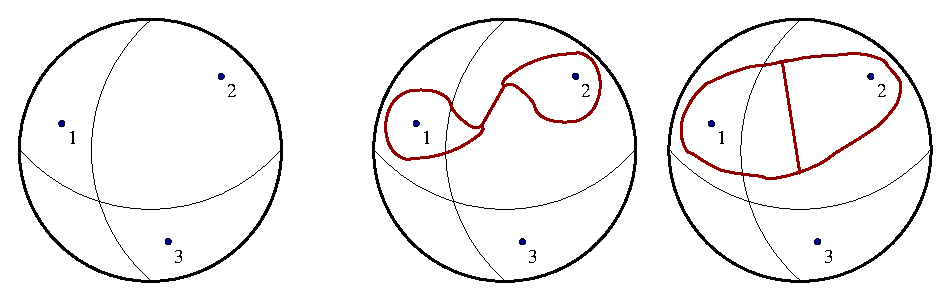
\includegraphics[width=\textwidth]{sfera3}
  \caption{A thrice punctured sphere and two inequivalent
    deformation retracts.} 
  \label{fig:sphere-retracts}
\end{figure}
We look forward to refining this correspondence: let us introduce more
structure on the graph.
\begin{definition}
  \label{dfn:metric-ribbon-graphs}
  A metric ribbon graph is the data of a type (0,0) ribbon graph (see
  \csref{dfn:ribbon-graphs}) equipped with a real positive number
  $\ell_\alpha$ for each edge $\alpha$.
\end{definition}

One can use the cyclic order to ``fatten'' edges of a graph $\Gamma$ into
thin ribbons\footnote{Hence the names ``ribbon graph'' and
  ``fatgraph''.}  (see \csref{fig:fattening-edges}), so to obtain a
compact oriented Riemann surface with boundary $\tilde S(\Gamma)$.
Viceversa, any graph $\Gamma$, embedded in a oriented Riemann surface,
inherits a cyclic order from the orientation.
\begin{figure}[htbp]
  \begin{equation*}
    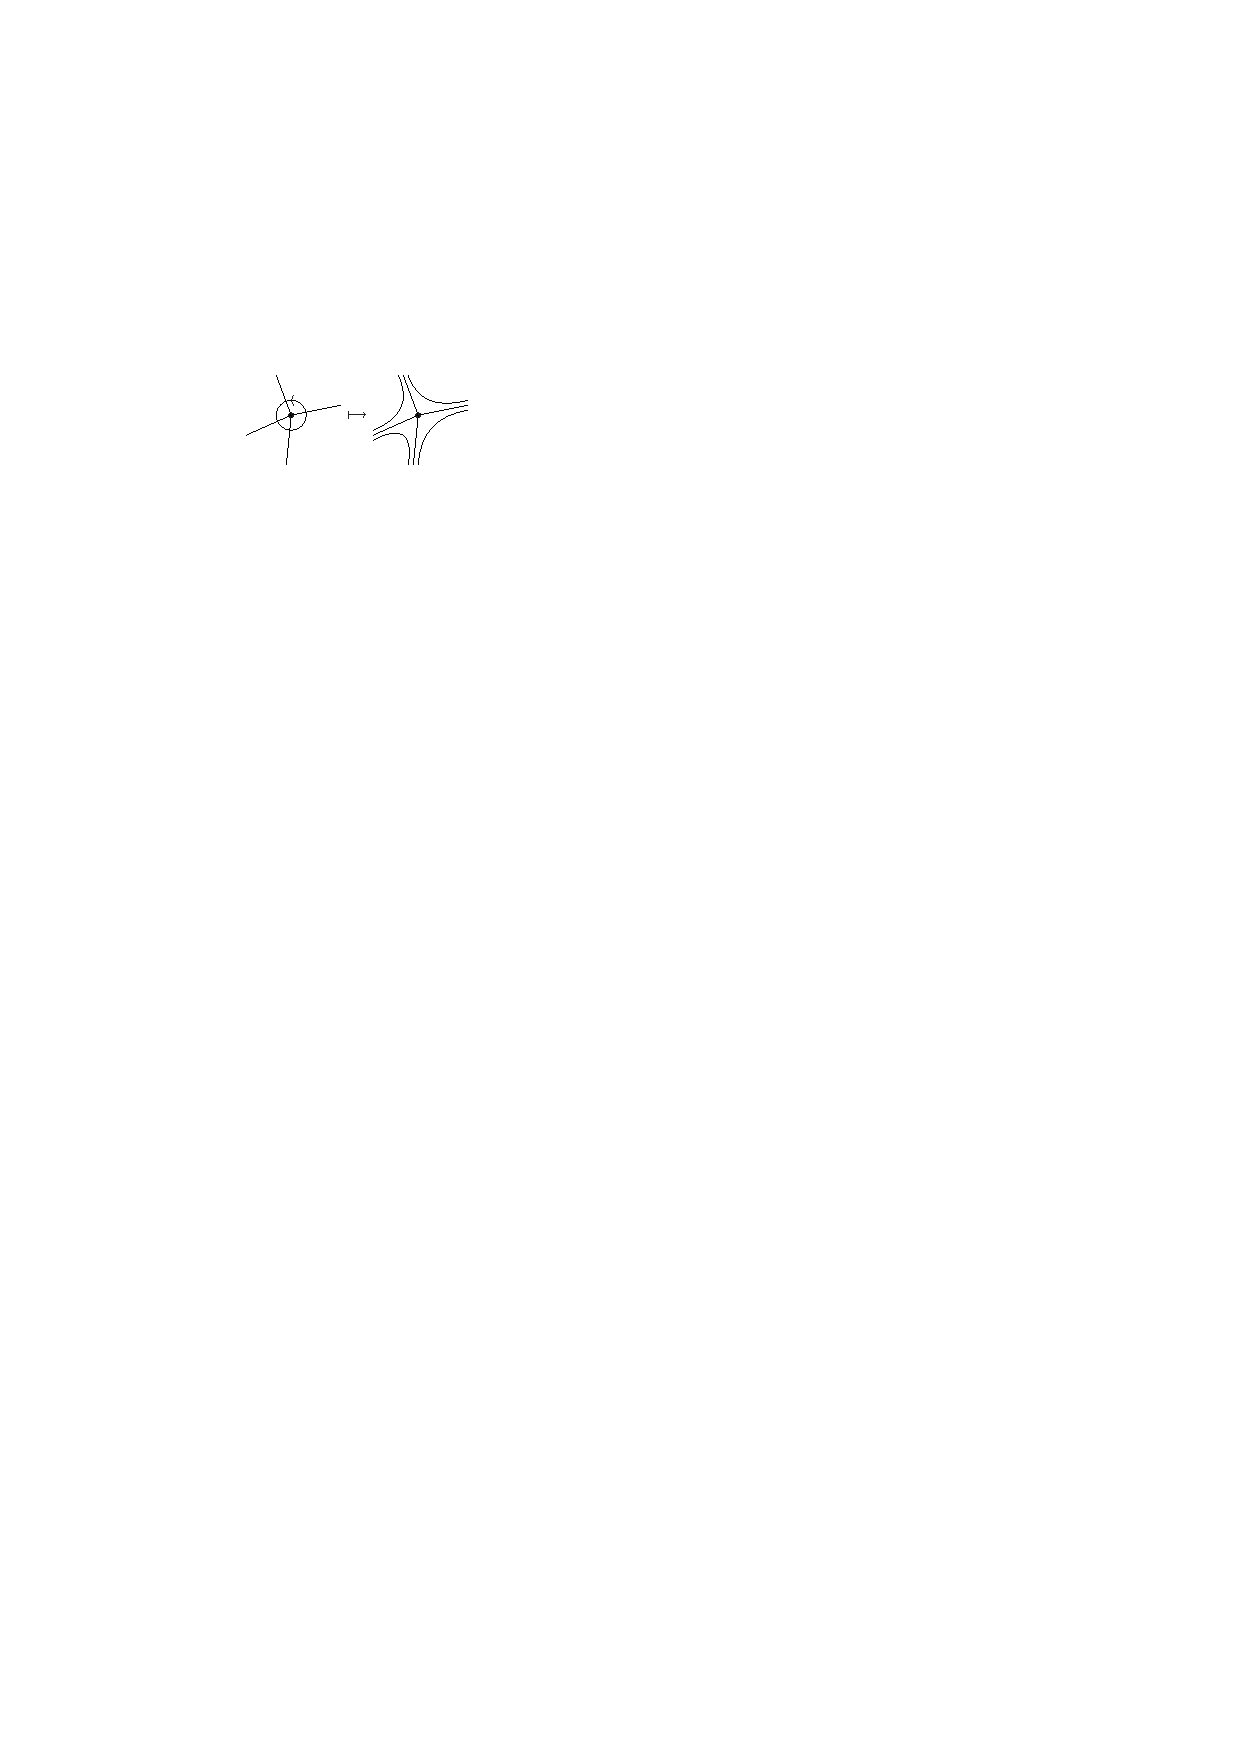
\includegraphics{fatten}
  \end{equation*}
  \caption{Fattening edges at a vertex with cyclic order.}
  \label{fig:fattening-edges} 
\end{figure} 
Now glue punctured disks alongside the boundary of $\tilde S(\Gamma)$ to
get a punctured Riemann surface $S(\Gamma)$. Obviously,
\begin{equation*}
  \chi(\Gamma) = \chi(S(\Gamma)) = 2 - 2g - n,
\end{equation*}
so we can define, for a ribbon graph $\Gamma$, the \emph{genus} $g$ and the
\emph{puncture number} $n$, as given by the above relation.

Notice that this fattening procedure actually selects some homological
$1$-cycles in $\Gamma$, those corresponding to the boundary components of
$\tilde S(\Gamma)$. By abuse of language, we shall call these $1$-cycles
``boundary components'' or ``holes'', for short.

Denote $\Vertices{\Gamma}$, $\Edges{\Gamma}$ and $\Holes{\Gamma}$ the
sets of vertices, edges and holes of a graph $\Gamma$. It will be
convenient to identify a hole $\beta$ with the set of edges it is made
of, and a vertex $\gamma$ with the set of edges incident to it.


\subsection{A complex structure on $S(\Gamma)$}
\label{sec:atlas}
Let us give the topological Riemann surface $S(\Gamma)$ a complex
structure, by means of a triangulation and an analytic atlas.

In the course of the construction of $S(\Gamma)$, two punctured disk
have been glued on the sides of an edge $\alpha \in \Edges{\Gamma}$: call
them $\alpha^+$ and $\alpha^-$. Let $T_\alpha^+$ and $T_\alpha^-$ be the triangles
delimited by $\alpha$ and the radii joining endpoints of $\alpha$ with the
puncture of $\alpha^\pm$. The collection $\{T_\alpha^\pm : \alpha \in \Edges{\Gamma}\}$
is a triangulation of $S(\Gamma)$.

Define an atlas of $S(\Gamma)$:
\begin{itemize}
\item for any edge $\alpha$, put $V_\alpha := (T_\alpha^+ \cup T_\alpha^-)^\circ$;
\item for any hole $\beta$, put $V_\beta := \bigl( \bigcup_{\alpha} T_\alpha \bigr)^\circ$
  for all $\alpha$ bounding $\beta$;
\item for any vertex $\gamma$, put $V_\gamma := \bigl( \bigcup_\alpha T_a^\pm \bigr)^\circ$
  for all $\alpha$ incident to $\gamma$.
\end{itemize}
\begin{figure}[btp]
    %% Figura atlas.fig
  \centering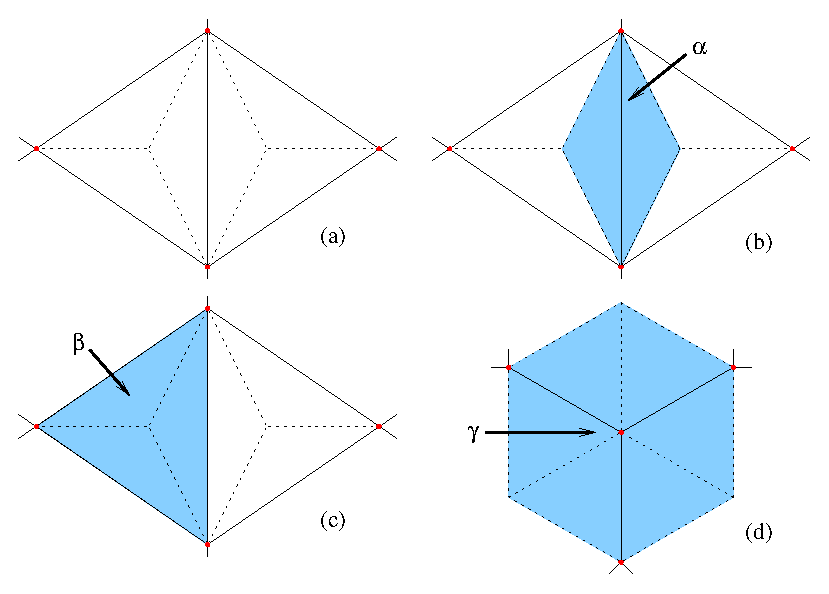
\includegraphics[width=\textwidth]{atlas}
  \caption{The open sets building an atlas of $S(\Gamma)$: (a) the
    triangulation built from a graph $\Gamma$; (b) the neighborhood
    $V_\alpha$ of an edge $\alpha$; (c) the neighborhood $V_\beta$ of a hole
    $\beta$; (d) the neighborhood $V_\gamma$ of a vertex $\gamma$.}
  \label{fig:atlas}
\end{figure}

Define charts on the open sets $V$ (see Figure~\ref{fig:charts}):
\begin{itemize}
\item for any edge $\alpha$, pick a homeomorphism $f_\alpha: V_\alpha \to \{ z \in \setC
  : 0 < \Re z < \ell_\alpha \}$;
\item for any hole $\beta$, bounded by edges $\alpha_1$, $\alpha_2$ and $\alpha_3$,
  pick a homeomorphism $f_\beta: V_\beta \to \{ \abs{z} < \rho \}$, where $\rho =
  (\ell_{\alpha_1} + \ell_{\alpha_2} + \ell_{\alpha_3}) / 2\pi$.
\item for any vertex $\gamma$, pick a homeomorphism $f_\gamma: V_\gamma \to \setC$.
\end{itemize}
\begin{figure}[htbp]
    %% Figura charts.fig
  \centering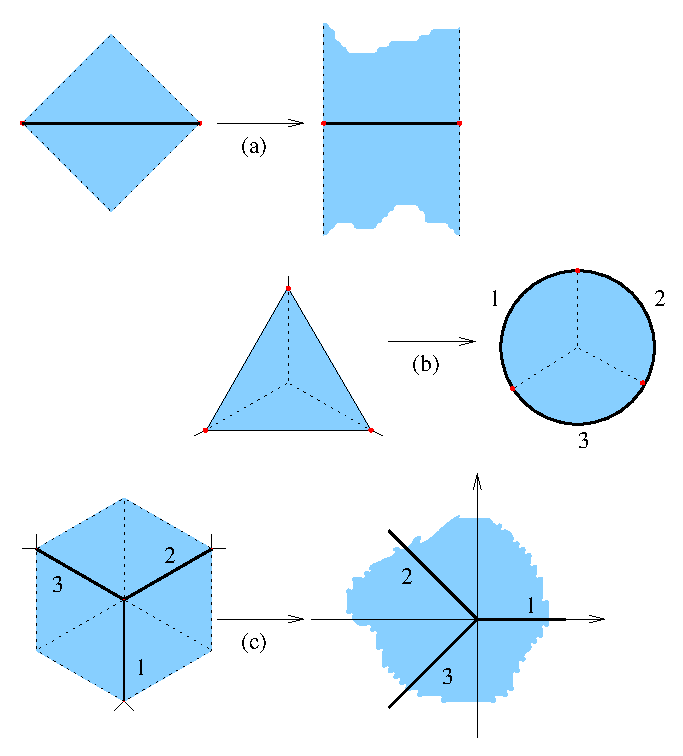
\includegraphics{charts}
  \caption{Local charts on the atlas: (a) any open set $V_\alpha$
    maps to a strip in the complex plane; (b) any open set $V_\beta$
    maps to a disk; (c) any open set $V_\gamma$ maps to the complex
    plane itself.}
  \label{fig:charts}
\end{figure}
These choices are subject to the condition that transition functions
satisfy the following:
\begin{itemize}
\item if $\alpha$ is an edge bounding the hole $\beta$, then $f_\beta \circ
  f_\alpha^{-1} = \exp (2\pi\I z / p_\beta)$ with $p_\beta := \sum_{\alpha \in \beta} \ell_\alpha$
  (\emph{perimeter} of the hole $\beta$);
\item if $\alpha$ is incident to a vertex $\gamma$, then $f_\gamma \circ f_\alpha^{-1} =
  c \cdot z^{2/(m+2)}$, up to a complex constant of modulus $1$, where
  $m$ is the valence of the vertex $\gamma$.
\end{itemize}

In the end, we have come upon a complex analytic structure on
$S(\Gamma)$, which depends on the perimeters $p_1, \ldots, p_n$ of holes $\beta_1,
\ldots, \beta_n$. By varying these (real positive) parameters, one can vary
the complex structure on $S(\Gamma)$; this will allow for an alternative
construction of the moduli space $\M_{g,n}$.


\subsection{The Strebel construction}
\label{sec:strebel}
A theorem proved by K. Strebel in the 1960's provides an inverse
route to the construction of smooth complex curves from ribbon
graphs. 

\begin{definition}
  A quadratic differential $q$ on a Riemann surface $S$ is a
  (meromorphic) section of $(T^*)\tp2$.
\end{definition}
The set of vectors in $T_zS$ on which $q$ takes real non-negative
values form a real line in $T_zS$: therefore, they make up a foliation
on $S$. The non compact leaves together with zeroes of $q$ form the
``critical locus'' of $q$.

Every quadratic differential $q$ induces a metric (away from the
critical locus) by $ds^2 = \abs{q(z)} \cdot \abs{\ud z}$.

\begin{theorem}[Strebel, {\cite[Theorem 23.2 and
    23.5]{strebel;quadratic-differentials;1983}}] For all complex
  analytic curve $S$, with $n$ marked points $x_1, \ldots, x_n$, and any
  assignment of real positive numbers $p_1, \ldots, p_n$, there exists one
  and only one meromorphic quadratic differential $q$ such that:
  \begin{enumerate}
  \item the critical locus of $q$ is a graph $\Gamma$ embedded in $S$;
  \item the poles of $q$ reside in the marked points $x_1, \ldots, x_n$
    with second residue $p_1, ..., p_n$;
  \item every compact leaf rounding $x_i$ has length $p_i$ in the flat
    metric induced by $q$.
  \end{enumerate}
\end{theorem}
The critical graph $\Gamma$ inherits a structure of ribbon graph with
metric from the ambient surface $S$; the length of an edge $\alpha$ is the
one measured in the metric induced by the quadratic
differential. Furthermore, Strebel's theory states that $\Gamma$ has a
vertex of valence $k+2$ where $q$ has a zero of order $k$, therefore,
vertices of $\Gamma$ have valence $\geq3$.

Since the markings $x_1, \ldots, x_n$ are \emph{ordered}, $\Gamma$ has an
additional structure of \emph{numbered} graph, that is, it is endowed
with a bijection $h: \Holes{\Gamma} \to \{1, \ldots, n\}$. 
\begin{definition}
  \label{dfn:strebel-graphs}
  Define a category $\Strebel[g,n]$, whose objects are metric numbered
  ribbon graphs with genus $g$ and $n$ holes, all whose vertices have
  valence $\geq3$ (call them ``Strebel graphs'', for short) .  Morphisms
  $\Gamma \to \Gamma'$ are compositions of graph isomorphisms and contractions of
  an edge $\alpha \in \Edges{\Gamma}$.
\end{definition}

Let $\Gamma$ be a Strebel graph of genus $g$ with $n$ holes.  A topological
cell $\Delta_\Gamma \subseteq \M_{g,n}$ is spanned when varying the metric data
$(\ell_\alpha)_{\alpha \in \Edges{\Gamma}}$; gluing these cells one recovers the
whole $\M_{g,n}$. We present here a quick construction, apparently due
to Kontsevich \cite{kontsevich;intersection-theory;1992}.

Call a set $X \subseteq \Edges{\Gamma}$ negligible whenever it is \emph{not} the
support of any non-trivial homological cycle.  Define
\begin{equation*}
  \label{eq:kontsevich-3}
  M(\Gamma) := \{ \ell: \Edges{\Gamma} \to \setR_{>0} | \text{the zero set of $\ell$ is negligible}\}.
\end{equation*}
It is a contravariant functor from the category of Strebel graphs to
the category of topological spaces: if $\Gamma'$ is obtained from $\Gamma$ by
contracting the edge $\alpha_0$, then
\begin{equation*}
  M(\Gamma') = \{ \ell \in M(\Gamma) | \ell_\alpha = 0 \}.
\end{equation*}
\begin{definition}
  The combinatorial moduli space of smooth algebraic curves is the
  direct limit of the functor $M$:
  \begin{equation*}
    \Mcomb_{g,n} := \varinjlim M(\Gamma),
  \end{equation*}
  with $\Gamma$ in the category $\Strebel[g,n]$ of Strebel graphs.
\end{definition}
\begin{remark}
  $\Mcomb_{g,n}$ is obtained by gluing orbicells $M(\Gamma)$ (quotient of
  a topological cell by $\Aut \Gamma$) alongside the boundary (if $\Gamma'$ is a
  contraction of $\Gamma$, then $M(\Gamma')$ is a face of $M(\Gamma)$). Therefore,
  $\Mcomb_{g,n}$ is a orbifold.
\end{remark}

It is easy to check that any $[\Gamma, \ell] \in \Mcomb_{g,n}$ has a unique
representative such that $\ell_\alpha > 0$ for all $\alpha \in \Edges{\Gamma}$.
The perimeter maps $p_\beta: \Mcomb_{g,n} \to \setR_{>0}$ are well-defined;
write $p_j$ for the perimeter of the $j$-th hole.

The construction of $\Mcomb_{g,n}$ can be done with slightly changed
rules: if we define a set $X \subseteq \Edges{\Gamma}$ to be negligible iff it
does not contain all edges bounding a hole, then we can define a
contrafunctor $\overline{M}(\Gamma)$ and a topological space:
\begin{equation*}
  \label{eq:kontsevich-4}
  \Mbarcomb_{g,n} := \varinjlim \overline{M}(\Gamma).
\end{equation*}
$\Mbarcomb_{g,n}$ turns out to be a compactification of the orbifold
$\Mcomb_{g,n}$. 

\begin{theorem}[Mumford, Harer, Penner, Thurston;
  \cite{looijenga;cellular-decomposition}] 
  The Strebel construction defines morphisms
  \begin{equation*}
    \M_{g,n} \times \setR_{>0}^n \to \Mcomb_{g,n}, \qquad \Mbar_{g,n} \times
    \setR_{>0}^n \to \Mbarcomb_{g,n}.
  \end{equation*}
  The first of these is a homeomorphism and, more, an orbifold
  equivalence. The inverse map
  \begin{equation*}
    \Mcomb_{g,n} \to \M_{g,n} \times \setR_{>0}^n \to \setR_{>0}^n
  \end{equation*}
  is the perimeter map $\pi := (p_1, \ldots, p_n)$.  
\end{theorem}

For any given $p^\circ = (p_1^\circ, \ldots, p_n^\circ) \in \setR_{>0}^n$, the fiber
$\pi^{-1}(p^\circ)$ is isomorphic to $\M_{g,n}$, thus, $\pi$ induces a
triangulation of $\M_{g,n}$.

The cell $M(\Gamma)$ has real dimension $\card{\Edges{\Gamma}}$; therefore,
cells of maximal dimension are given by graphs with all vertices of
valence $3$. The union of these cells is a dense subset of
$\Mcomb_{g,n}$ with non-void interior.


\section{Kontsevich' calculations}
\label{sec:calculation}

Kontsevich' praised calculation provides the bridge between the
combinatorial approach to the geometry of moduli spaces and the
Feynman diagrams theory of matrix integrals. In view of later
applications \cite{witten;kontsevich-model}, this should be
regarded as the very important result in Kontsevich' proof of Witten's
conjecture.


\subsection{Combinatorial expression of Witten's classes}
\label{sec:wittens-classes-comb}
\FIXME{Tutta questa sezione pu{\`o} ridursi al solo \csref{thm:comb-bundle}?}
Let $C_N$ be the cyclic group of order $N$. Define $B_N := \setR^N / C_N$
to be the orbicell of sequences $[l_1, \ldots, l_N]$ of non-negative real
numbers modulo cyclic permutations, endowed with the quotient
topology. There exist $N+1$ natural inclusion maps $\iota_j: B_N \ni [l_1,
\ldots, l_N] \mapsto [l_1, \ldots, l_{j-1}, 0, l_j, \ldots, l_N] \in B_{N+1}$; these
make $\{B_N, \iota\}$ into an inductive family of topological spaces.
Finally, define
\begin{equation*}
  B := \varinjlim B_N.
\end{equation*}
Every point of $B$ has a unique representative $[l_1, \ldots, l_N]$
enjoying $l_j > 0$ for all $j$. It is convenient to introduce
``barycentric'' coordinates $[p; s_1, \ldots, s_N]$ given by $p := \sum l_j$
and $s_j := l_j/p$.

Define $U_N := \{ (p; \Theta) | p>0, \ \Theta\subseteq S^1, \card{\Theta} = N\}$; give it
the subspace topology of $(S^1)^N$. The group $S^1$ acts on every
$U_N$, and there are surjections $f_\sigma$, for $\sigma \in C_N$:
\begin{multline*}
  E_N := \{ (p; \theta_1, \ldots, \theta_N) | 0\leq \theta_1 < \ldots < \theta_N < 1\} \ni (p;
  \theta_1, \ldots, \theta_N) 
  \\
  \stackrel{f_\sigma}{\longmapsto} [p; \E^{\I\theta_1}, \ldots,
  \E^{\I\theta_N}] \in U_N.
\end{multline*}
Put $U_{\leq N} := \bigcup_{j \leq N} U_j$; the inclusions $U_{\leq N} \hookrightarrow U_{\leq
  N+1}$ define an inductive family. Finally, define:
\begin{equation*}
  E := \varinjlim U_{\leq N}.
\end{equation*}
The coordinate patch $E^\sigma_N := (E_N, f_\sigma)$ covers the stratum $U_N
\subseteq E$.

Define projection maps $E^\sigma_N \to B_N$ by 
\begin{equation*}
  E_N^\sigma \ni (p; \theta_1, \ldots, \theta_N) \mapsto [p; \theta_2 - \theta_1, \theta_3 - \theta_2, \ldots, 1
  + \theta_1 - \theta_N] \in B_N;
\end{equation*}
they can be glued into a continuous surjection $\ell: E \to B$, whose
fibers are the orbits of the action of $S^1$ on $E$. It is easy to
check that the spaces $B$ and $E$ are contractible and that $E$ is an
$S^1$-bundle on $B$.
\begin{lemma}
  \label{thm:comb-bundle}
  There exists a differential $1$-form $\alpha$ on $E$ such that:
  \begin{enumerate}
  \item on any patch $E^\sigma_N$, $\alpha$ is given by
    \begin{equation*}
      \alpha := \sum_{j=1}^N s_j \ud\theta_j, \qquad s_j= \theta_{j+1} - \theta_j, \ s_N = 1 +
      \theta_1 - \theta_N;
    \end{equation*}
  \item $\alpha$  restricts to the angle form on the fibers of $\ell$.
  \item   the differential $\ud\alpha$ relates to the first Chern class of $E$
    according to $\ud\alpha = -s^*c_1(E)$;
  \item the differential $\ud\alpha$ is the pull-back on $E$ of a $1$-form $\omega$
    on $B$, defined by:
    \begin{equation*}
      \omega = \sum_{1\leq j\leq k\leq N-1} \ud s_j \land \ud s_k.
    \end{equation*}
  \end{enumerate}
\end{lemma}
\begin{proof}
  Items 1)--2) may be proved by direct calculation; 3) is a standard
  result: consult, for instance, \cite{bott-tu}; finally 4) can be
  seen by induction on $N$.
\end{proof}

Now, the turnkey observation is that points in $B$ may be regarded as
circles with $N$ points marked, that is, ribbon graphs with only
2-valent vertices; so, we can define maps $b_j: \Mcomb_{g,n} \to B$ which
send the $j$-th hole $\beta$ (made of edges $\alpha_1$, \ldots, $\alpha_N$) to the
point $[\ell_{\alpha_1}, \ldots, \ell_{\alpha_N}] \in B_N \subseteq B$. 
\begin{theorem}[Kontsevich, {\cite[Theorem
    2.3]{kontsevich;intersection-theory;1992}}]
  The map $\M_{g,n} \times \setR^n \to B$, which is the composition of the
  maps $b_j$ with the isomorphism $\M_{g,n} \times \setR^n \simeq
  \Mcomb_{g,n}$, extends continuously to $\Mbar_{g,n} \times \setR^n$. The
  inverse image of the bundle $E \to B$ under $b_j$ is naturally
  isomorphic to the $S^1$-bundle associated with the complex line
  bundle ${\Lb}_j$. The pull-back $\omega_j$ of the form $\omega$ (defined in
  \csref{thm:comb-bundle}) under $b_j$ represents the class
  $c_1({\Lb}_j)$. 
\end{theorem}


\subsection{Kontsevich' Main Identity}
\label{sec:KMI}

Results from the previous section allow us to write
\begin{equation}
  \label{eq:kontsevich-6}
  \langle \tau_{\nu_1} \cdots \tau_{\nu_n} \rangle = \int_{\pi^{-1}(p^\circ_*)} \omega^{\nu_1} \land \cdots
  \land \omega^{\nu_n},
\end{equation}
but actually, as Kontsevich proved, one can draw a much stronger
conclusion. 

\begin{theorem}[Kontsevich' Main Identity]
  Let $\RG[g,n]$ be the set of isomorphism classes of numbered
  ribbon graphs with genus $g$ and $n$ boundary components. If
  $\alpha$ is an edge of a graph $\Gamma \in \RG[g,n]$, let $\alpha^+$
  and $\alpha^-$ be the \emph{numbers} assigned to the two holes on
  the sides of $\alpha$. For complex indeterminates $\lambda_1$,
  \ldots, $\lambda_N$, the following relation holds:
  \begin{multline*}
    \sum_\nu \langle \tau_{\nu_1} \cdots \tau_{\nu_n} \rangle \prod_{j=1}^n \frac {(2\nu_j - 1)!!}
    {\lambda_j^{2\nu_j + 1}} = \sum_{\Gamma \in \RG[g,n]} \frac
    {2^{-\card{\Vertices{\Gamma}}}} {\card{\Aut \Gamma}} \prod_{\alpha \in \Edges{\Gamma}}
    \frac {2} {\lambda_{\alpha^+} + \lambda_{\alpha^-}}, 
    \\ \sum \nu = 3g - 3 + n.
  \end{multline*}
\end{theorem}
\begin{proof}
  Define a differential $2$-form on $\Mbarcomb_{g,n}$ by $\Omega := \sum
  p_j^2 \omega_j$. Recall that the metric data $(\ell_\alpha)_{\alpha \in \Edges{\Gamma}}$
  define local coordinates on the orbicell $M(\Gamma)$; it is easy to check
  that the restriction of $\Omega$ to the fibers of $\pi$ is non-degenerate
  and has constant coefficients in the coordinates $\ell_\alpha$. 
  
  Therefore, $\Omega^q$, with $q := 3g -3 + n = \dim \M_{g,n}$, is a
  volume form on the fibers of $\pi$.  The product $\Omega^q/q! \times
  dp_*$ is a volume form on the whole $\Mcomb_{g,n}$ and one can check
  that the ratio of measures
  \begin{equation*}
    \rho := (\Omega^q/q! \times {dp_1 \land \cdots \land dp_n}) / (d\ell_1 \land \cdots \land d\ell_N) 
  \end{equation*}
  is a \emph{constant}, independent of $\Gamma$ (that is, local expression
  in a cell $M(\Gamma)$), and depending only on $g$ and $n$; more precisely,
  \begin{equation*}
    \rho = 2^{2n + 5g - 5} = 2^{q - \card{\Vertices{\Gamma}} + \card{\Edges{\Gamma}}}.
  \end{equation*}
  The proof of this last fact is quite technical and intricate: see
  \cite[Appendix C]{kontsevich;intersection-theory;1992}.

  Consider the integral
  \begin{equation*}
    I := \int_{\Mbarcomb_{g,n}} \Omega^q/q! \cdot \exp(-\sum \lambda_j p_j) dp_*.
  \end{equation*}
  On the one hand, from formula
  \begin{equation*}
    \int_{\pi^{-1}(p^\circ_*)} \Omega^q/q! = (1/q!) \cdot \int_{\pi^{-1}(p^\circ_*)} \bigl( p_1^2
    c_1({\Lb}_1) + \cdots + p_n^2 c_1({\Lb}_n) \bigr)^q,
  \end{equation*}
  and \eqref{eq:kontsevich-6}, one can compute:
  \begin{equation}
    \label{eq:8}
    I = \sum_\nu \langle \tau_{\nu_1} \cdots \tau_{\nu_n} \rangle \prod_{j=1}^n (2\nu_j)!!
    \lambda_j^{-2\nu_j -1}, \qquad \sum \nu_j = q.
  \end{equation}

  On the other hand, since the ratio $\rho$ is constant on all of
  $\Mcomb_{g,n}$, then 
  \begin{equation*}
    I = \rho \cdot \int_{\Mcomb_{g,n}} \exp(-\sum \lambda_j p_j) \abs{d\ell_1 \land \cdots \land d\ell_N}.
  \end{equation*}
  Since the Strebel triangulation of $\Mcomb_{g,n}$ is indexed by
  ribbon graphs, we can immediately say that the above integral is a
  sum of terms corresponding to ribbon graphs; what is more, since the
  integral can be computed by restricting to an open stratum, we may
  limit the sum to trivalent ribbon graphs only. A little
  combinatorics shows that, for a fixed trivalent ribbon graph
  $\Gamma$,
  \begin{equation*}
    \exp( -{\textstyle \sum} \lambda_j p_j) = \prod_{\alpha \in \Edges{\Gamma}} \exp -\ell_\alpha(\lambda_{\alpha^+} +
    \lambda_{\alpha^-}),
  \end{equation*}
  so that we can finally compute:
  \begin{equation}
    \label{eq:7}
    I = \sum_{\Gamma \in \RG[g,n]} \frac {1} {\card{\Aut \Gamma}} \prod_{\alpha \in
      \Edges{\Gamma}} \frac{1} {\lambda_{\alpha^+} +
      \lambda_{\alpha^-}}.
  \end{equation}

  Multiply by $2^{-q}$ and equate \eqref{eq:7} and \eqref{eq:8} to get
  the thesis.
\end{proof}

Take a formal sum, over all $g,n$, of the LHS of the Main
Identity, and substitute $\Lambda_{j_k}$ for $\lambda_k$: 
\begin{multline}
  \label{eq:KMI-F}
  F(t_0(\Lambda), t_1(\Lambda), \ldots) = \sum_{n, \nu_1, \ldots, \nu_n} 1/n! \langle \tau_{\nu_1}
  \cdots \tau_{\nu_n} \rangle t_{\nu_1}(\Lambda) \cdots t_{\nu_n}(\Lambda)
  \\
  = \sum_{n, \nu_1, \ldots, \nu_n} (-1)^n/n! \langle \tau_{\nu_1} \cdots \tau_{\nu_n} \rangle
  \sum_{1 \leq j_1, \ldots, j_n \leq N} \prod_{k=1}^n (2\nu_k -1)!! \Lambda_{j_k}^{-2\nu_k
    - 1}
  \\
  = \sum_{\substack{\Gamma \in \Strebel[g,n] \\ c: \Holes{\Gamma} \to \{1,
      \ldots, N\}}} \frac {(\I/2)^{\card{\Vertices{\Gamma}}}} {\card{\Aut
      \Gamma}} \prod_{\alpha \in \Edges{\Gamma}} \frac{2} {\lambda_{c(\alpha^+)} +
    \lambda_{c(\alpha^-)}}.
\end{multline}
So we have expressed $F(t_*(\Lambda))$ as a sum of analytic expressions
computed from graphs; up to our astonishment, the right-hand side
comes out to be a Feynman diagrams expansion of a matrix integral.


\section{The 't~Hooft-Kontsevich model}
\label{sec:matrix-models}
\everyxy={0,<2em,0em>:,(0,0.5),} % scala per i diagrammi

The Kontsevich matrix model for 2D quantum gravity, first defined in
\cite{kontsevich;intersection-theory;1992}, provides a bridge from
equation~\eqref{eq:KMI-F} to Hermitian matrix integrals. The
Kontsevich model embodies the ``standard matrix model'' of 't~Hooft as
a particular case. 

A cyclic algebra structure is introduced on the vector space
$\Hermitian[N]$ of $N\times N$ Hermitian matrices; then we can apply the
general results of \csref{cha:fd} on Feynman diagrams.

Let $V$ be an $N$-dimensional Hilbert space. The space $\End(V)$
has a natural Hermitian inner product
\begin{equation*} 
  \inner{X}{Y}\joinrel:=\tr(X^*Y),
\end{equation*}
which induces the standard Euclidean inner product $\inner{X}{Y} =
\tr(XY)$ on the real subspace
\begin{equation*}
  \Hermitian[N]\joinrel:=\{X\in \End(V) | X^*=X\}
\end{equation*}
of Hermitian operators.  

For any positive definite Hermitian operator $\Lambda$, we can define
a new Euclidean inner product on $\Hermitian[N]$ by
\begin{equation*}
  \inner[\Lambda]{X}{Y} \joinrel:= 
  \onehalf \left(\tr(X\Lambda Y) + \tr(Y\Lambda X)\right).
\end{equation*}

Now, define cyclic tensors
\begin{equation*}
  T_k:\Hermitian[N]\tp{k} \ni X_1 \otimes X_2 \otimes \dots \otimes X_k 
  \mapsto 
  \tr(X_1X_2\cdots X_k) \in \setC;
\end{equation*}
These $T_k$, together with the inner product $\inner[\Lambda]{-}{-}$,
define a cyclic algebra structure on $\Hermitian[N]_\setC\simeq \End(V)$
called the Kontsevich model. A graphical calculus $Z$ for the Kontsevich
model is ~defined on the PROP $\RG$ of ribbon graphs.

\begin{lemma}\label{thm:KMI-Z}
  The following formula holds:
  \begin{equation*}
    \label{eq:KM}
    Z (\Gamma) =
    \sum_{c} \prod_{\ell\in
      \Edges{\Gamma}} \frac{2}{\Lambda_{c(\ell^+)} + \Lambda_{c(\ell^-)}},
    \qquad c\colon\Holes{\Gamma} \to \{1, \dots, N\}
  \end{equation*}
  where $\Lambda_1, \dots, \Lambda_N$ are the eigenvalues of $\Lambda$, $c$ runs
  over all colorings of holes of $\Gamma$ in $N$ colors, and $\ell^+$,
  $\ell^-$ are the two holes bounded by the edges $\ell$ (they are not
  necessarily distinct).
\end{lemma}
\begin{proof}
  To evaluate $Z(\Gamma)$ we need an explicit expression for the Casimir
  element $\coev_{\Hermitian[N],\Lambda}(1)$ of the cyclic algebra $(
  \Hermitian[N]_\setC, \inner[\Lambda]{-}{-}, T_1, T_2, \dots)$.  Since $\Lambda$
  is Hermitian positive definite, there exists an orthonormal basis
  $\{e_i\}$ of $V$ in which
  \begin{equation*}
    \Lambda=\diag(\Lambda_1,\Lambda_2\dots,\Lambda_N),
  \end{equation*}
  for some $\Lambda_i$ positive real numbers. Any choice of a like basis
  induces an identification of $V$ with $\setC^N$, and, consequently,
  of $\End(V)$ with the space $M_N(\setC)$ of $N \times N$ complex
  matrices. Let $\{E_{ij}\}$ be the canonical basis for $M_N(\setC)$:
  \begin{equation*}
    (E_{ij})_{kl}=\delta_{ik}\delta_{jl}.
  \end{equation*}
  A basis for $\Hermitian[N]$ is given by matrices
  \begin{equation*}
    e_{ij}=\begin{cases}
      \frac{1}{\sqrt{2}} (E_{ij}+E_{ji}) &\text{if $i<j$,}\\
      E_{ii}                             &\text{if $i=j$,}\\
      \sqrt{-\onehalf} (E_{ij}-E_{ji})   &\text{if $i>j$.}
    \end{cases}
  \end{equation*}
  It is orthonormal with respect to the inner product
  $\inner{-}{-}$, whereas 
  \begin{equation*}
    \inner[\Lambda]{e_{ij}}{e_{kl}}
    = \frac{\Lambda_i + \Lambda_j}{2} \delta_{ij,kl},
  \end{equation*}
  i.e., the matrix of $\inner[\Lambda]{-}{-}$ with respect to the
  basis $\{e_{ij}\}$ is
  \begin{equation*}
    g = \diag\left(\left\{ \frac{\Lambda_i + \Lambda_j}{2}
      \right\}\right).
  \end{equation*}
  So we get the following expression for the Casimir element:
  \begin{equation*}
    \coev_{\Hermitian[N],\Lambda}(1) = \sum_{i,j}
    \frac{2}{\Lambda_i+\Lambda_j} e_{ij} \otimes e_{ij}.
  \end{equation*}
  Rewrite this identity as:
  \begin{align*}
    \coev_{\Hermitian[N],\Lambda}(1)&=\sum_{i}\frac{1}{{\Lambda_i}}e_{ii}\otimes
    e_{ii}+\sum_{i<j}\frac{2}{{\Lambda_i+\Lambda_j}}e_{ij}\otimes
    e_{ij}+\sum_{i>j}\frac{2}{{\Lambda_i+\Lambda_j}}e_{ij}\otimes
    e_{ij}\\
    &=\sum_{i}\frac{1}{{\Lambda_i}}e_{ii}\otimes
    e_{ii}+\sum_{i<j}\frac{2}{{\Lambda_i+\Lambda_j}}(e_{ij}\otimes
    e_{ij}+e_{ji}\otimes
    e_{ji}),
  \end{align*}
  but, for $i<j$,
  \begin{align*}
    e_{ij}\otimes e_{ij} &+ e_{ji}\otimes e_{ji} = \\
    &\qquad + \frac{1}{
      2}(E_{ij}\otimes E_{ij} + E_{ij}\otimes E_{ji} + E_{ji}\otimes
    E_{ij}+E_{ji}\otimes E_{ji})\\
    &\qquad - \frac{1}{ 2}(E_{ij}\otimes E_{ij} - E_{ij}\otimes E_{ji} -
    E_{ji}\otimes
    E_{ij}+E_{ji}\otimes E_{ji})\\
    &= E_{ij}\otimes E_{ji} + E_{ji}\otimes E_{ij}.
  \end{align*}
  So,
  \begin{multline}\label{eq:casimir}
    \coev_{\Hermitian[N],\Lambda}(1)=
    \sum_{i}\frac{1}{{\Lambda_i}}E_{ii}\otimes
    E_{ii}+\sum_{i<j}\frac{2}{{\Lambda_i+\Lambda_j}}(E_{ij}\otimes E_{ji} + E_{ji}\otimes E_{ij})\\
    = \sum_{i,j}\frac{2}{{\Lambda_i+\Lambda_j}}E_{ij}\otimes E_{ji}.
  \end{multline}

  According to  standard graphical calculus rules, evaluation
  $Z(\Gamma)$ is performed through the correspondence
  \begin{equation*}
    {\xy*!LC\xybox{\rgvertex7\loose1\loose2\missing3%
        \loose4\loose5\missing6\loose7}\endxy}
    \leftrightarrow
    T_k,
    \qquad
    {\xy\vloop-\endxy}
    \leftrightarrow
    \coev_{\Hermitian[N],\Lambda}(1).
  \end{equation*}
  If we introduce the notation
  \begin{equation*}
    {\xy\vloop-,(0.05,0.5)*\txt{${}_i\
        {}_j$},(1,0.5)*\txt{${}_j\
        {}_i$}\endxy}=\frac{2}{\Lambda_i+\Lambda_j} E_{ij}\otimes E_{ji},
  \end{equation*}
  then we can depict \eqref{eq:casimir} as
  \begin{equation*}
    {\xy\vloop-\endxy}
    = \sum_{i,j}
    {\xy\vloop-,(0.05,0.5)*\txt{${}_i\
        {}_j$},(1,0.5)*\txt{${}_j\ {}_i$}\endxy},
  \end{equation*}
  which turns $Z(\Gamma)$ into a sum of ribbon graphs equipped with a
  number in $\{1, \dots, N\}$ on each side of every edge, and
  operators $T_k$ on each $k$-valent vertex.

                                %  The map $T_k$ is the restriction of a map $T_k$ defined on
                                %  $M_N(\setC)$, namely, the trace of a $k$-fold product. We have
  Since
  \begin{equation}\label{eq:vertices}
    T_k(E_{i_1j_1}\otimes E_{i_2j_2}\otimes\cdots\otimes
    E_{i_{k}j_k})=\delta_{j_1i_2}\delta_{j_2i_3}\cdots
    \delta_{j_{k-1}i_k}\delta_{j_ki_1},
  \end{equation}
                                %  Therefore,
  the only graphs that give non-zero contribution to the sum
  giving $Z(\Gamma)$ are the ones whose boundary components have the same
  index on all edges --- that is, we need only account for graphs
  equipped with a map $c\colon\Holes{\Gamma} \to \{1, \dots, N\}$.  An edge whose
  sides are indexed $i,j$ brings in a factor $2/(\Lambda_i+\Lambda_j)$; combining
  this with \eqref{eq:vertices}, we can conclude the proof.
\end{proof}

\begin{example}[The standard matrix model]
  Take $\Lambda = I$; formula \eqref{eq:KM} specializes to 
  \begin{equation*}
    Z(\Gamma) = \sum_{c} \prod_{\ell\in \Edges{\Gamma}} \frac{2}{\Lambda_{c(\ell^+)} +
      \Lambda_{c(\ell^-)}}
    = \sum_c 1 = N^{\card{\Holes{\Gamma}}}.
  \end{equation*}
  Therefore, according to \csref{thm:FRT},
  \begin{equation}
    \int_{\Hermitian[N]} \exp \left\{ \frac{1}{\hbar}\sum_{j=1}^{\infty}
      \frac{\tr X^j}{j}
    \right\} \ud\mu_I(X) = 
    \sum_\Gamma \frac{N^{\card{\Holes{\Gamma}}}} {\card{\Aut
        \Gamma}}\hbar^{-\card{\Vertices{\Gamma}}}.
  \end{equation}
  This is known as the ``standard matrix model'' in physics
  literature.
\end{example}

\begin{proof}[Proof of \csref{thm:kontsevich}]
  Asymptotic expansions commute with the integral sign, therefore
  \begin{equation*}
    \int_{\Hn} \exp (\I/6 \cdot \tr X^3) \ud\mu_\Lambda(X) \asymp \sum_m
    \frac{\I^m}{2^mm!} \correlator{(\tr
      X^3/3)^m}.
  \end{equation*}
  
  By \csref{thm:feynman}, the $m$-th summand in the right-hand side
  can be expanded into a sum over (possibly non-connected) colored
  ribbon graphs with $m$ trivalent vertices. As $m$ ranges over
  non-negative integers, we get the exponential of the right-hand side
  of \eqref{eq:KMI-F}, which completely proves \csref{thm:kontsevich}.
\end{proof}

\everyxy={/r24pt/:} % riportiamo la scala per i diagrammi

%%% Local Variables: 
%%% mode: latex
%%% TeX-master: "index"
%%% End: 

\RCSID $Id: construction.tex,v 1.2 2006/05/18 08:07:28 rmurri Exp $
%auto-ignore


\chapter{Construction of $A_\infty$ classes}
\label{cha:construction}

The construction of cohomology classes on $\M_{g,n}$ from the data of
an $A_\infty$-algebra was first sketched by Kontsevich in the 1994 talk at
ECM \cite{kontsevich;feynman}. It was further explained in
\cite{penkava-schwarz} and \cite{penkava;graph-complexes}, and
generalized in \cite{markl;cyclic} to graph complexes over any cyclic
operad.  A detailed exposition can be found in \cite{conant-vogtmann}.

Here we give a summary of the construction, restricted to the ribbon
graph triangulation of moduli spaces of curves.


\section{Arc-systems and their complexes}
\label{sec:arc-systems}

Harer \cite{harer;cohomological-dimension}, introduced the arc-systems
complex as a tool to calculate the (co)homology of the moduli space
$\M_{g,n}$.

Let $S_{g,n}$ be a topological compact oriented Riemann surface of
fixed genus $g$ with $n$ marked points $x_1, \ldots, x_n$.  Points in the
moduli space $\M_{g,n}$ can be regarded as equivalence classes
$(C,x,f)$ of a complex curve $C$ with a marking $x:\{1,\ldots,n\}\to C$ and a
homeomorphism $f:C\to S_{g,n}$ with the reference surface (see
\csref{rem:moduli-with-reference}).

If $\alpha$ is any arc in $C$, denote by $[\alpha]$ its isotopy class rel~$\{x_1,
\ldots, x_n\}$.

\begin{definition}
  An arc-system $[\alpha_1, \ldots, \alpha_k]$ of rank $k$ is an isotopy class
  rel~$\{x_1, \ldots, x_n\}$ of $k$ properly imbedded arcs $\alpha_i : [0,1] \to C$
  such that:
  \begin{itemize}
  \item every $\alpha_i$ has its endpoints in the set $\{x_1, \ldots, x_n\}$;
  \item if $i \neq j$, then $\alpha_i$ meet $\alpha_j$ only at endpoints, if at all;
  \item no $\alpha_i$ is null-homotopic rel~$\{x_1, \ldots, x_n\}$;
  \item no $\alpha_i$ is homotopic rel~$\{x_1, \ldots, x_n\}$ to $\alpha_j$, for $i \neq
    j$;
  \end{itemize}
\end{definition}

An arc-system $[\alpha_1, \ldots, \alpha_k]$ is said to \emph{fill up} the curve $C$
iff all connected components of $C - \bigcup\{\alpha_i\} - \{x_1,\ldots x_n\}$ are either
disks or punctured disks.

Arc-systems may be organized into a semi-simplicial complex.
\begin{definition}
  $X$ is the semi-simplicial complex having a simplex $\langle\alpha_1, \ldots, \alpha_k\rangle$
  for every rank $k$ arc-system $[\alpha_1, \ldots \alpha_k]$, with the proviso that
  $\langle\beta_1, \ldots, \beta_l\rangle$ is a face of $\langle\alpha_1, \ldots, \alpha_k\rangle$ iff $\{ [\beta_1], \ldots, [\beta_l]
  \} \subset \{ [\alpha_1], \ldots, [\alpha_k] \}$.
  
  $X_\infty$ is the subcomplex of all those simplices $\langle\alpha_1, \ldots, \alpha_k\rangle$
  that do not fill up the surface $S$.
\end{definition}

Let $\Delta^{n-1}$ be the $(n-1)$-dimensional geometric simplex.
\begin{theorem}[Harer, {\cite[Theorem
  1.3]{harer;cohomological-dimension}}]
There exists a $\Gamma_{g,n}$-equivariant homeomorphism $\Phi: \T_{g,n} \times
\Delta^{n-1} \to X \setminus X_\infty$.
\end{theorem}

Let $X^\circ$, $X_\infty^\circ$ be the first barycentric subdivisions of $X$
and $X_\infty$, respectively.

\begin{definition}
  Let $Y^\circ$ be the collection of simplices in $X^\circ$ having no face in
  $X_\infty^\circ$; equivalently, $\sigma_\bullet \in Y^\circ$ iff every vertex of $\sigma_\bullet$
  lies in $X^\circ \setminus X_\infty^\circ$.  $Y^\circ$ is a full subcomplex of $X^\circ$.
\end{definition}


%%% Local Variables: 
%%% mode: latex
%%% TeX-master: "index"
%%% End: 


\appendix
%auto-ignore


\chapter{Arrows-only description of Categories}
\label{cha:arrows}

It is convenient to have an arrows-only description of a category: in
this picture, an object $A \in \A$ is identified with the identity map
$\id_A \in \A(A, A)$.

According to \cite{lawvere;1965}, a category $\A$ can be described by
the following data:
\begin{itemize}
\item a set $\Hom\A$: the morphisms of $\A$;
\item a ternary relation $\Gamma(x,y;z)$, to be interpreted as ``$z$ is
  the composition of $x$ and $y$'';
\item set-theoretic maps $s,t: \Hom\A \to \Hom\A$ (called \emph{source}
  and \emph{target}), sending an arrow to its domain or codomain
  object,
\end{itemize}
which are tied by the following relations:
\begin{enumerate}
\item $\exists z: \Gamma(x,y;z) \Leftrightarrow s(x) = t(y)$; \label{item:A1}
\item $\Gamma(x,y;z) \land \Gamma(x,y;z') \Rightarrow z = z'$;
\suspend{enumerate}
--- by virtue of this we can adopt the more familiar notation $z = x\circ
y$ for $\Gamma(x,y; z)$, so that the next axioms look more like the
familiar properties of the composition product in a category ---
\resume{enumerate}
\item $z = x\circ y \Rightarrow s(z) = s(y) \land t(z) = t(x)$;
\item $(x\circ y) \circ z = x \circ (y \circ z)$;
\suspend{enumerate}
and, finally, two relations which are useful in characterizing
identity arrows:
\resume{enumerate}
\item $s \circ t = t \circ t = t$;
\item $t \circ s = s \circ s = s$.
\end{enumerate}

We are now ready to introduce objects of $\A$, i.e., identity
arrows. 
\begin{definition}\label{dfn:object}
  $A\in \A$ means that $A$ is a morphism of the category $\A$
  such that:
  \begin{enumerate}
  %\item $\exists x: [A = s(x)] \lor [A = t(x)]$,
  \item $A = s(A) = t(A)$, \label{item:AO1}
  \item $\forall x\forall y[ y = x \circ A \Rightarrow x = y] \land \forall x\forall y [
    x = A \circ y \Rightarrow x = y]$. \label{item:AO2} 
  \end{enumerate}
\end{definition}
Accordingly, we write $A$ for the identity morphism $\id_A$.

It is easy to deduce this characterization from the usual axioms of
category theory, but one can also assume it as a starting point for a
purely categorical foundation of set theory --- see
\cite{lawvere;1965}. 

In this framework, a functor $F: \A \to \category{B}$ is just a map $F:
\Hom\A \to \Hom\B$ such that
\begin{inparaenum}
\item $F(x \circ y) = F(x) \circ F(y)$, and
\item for any object $A \in \A$, $F(\id_A) = \id_{F(A)}$.
\end{inparaenum}

\begin{example}\label{xmp:braid-by-arrows}
  The $\catBraid$ category (\csref{xmp:braids}) is the category whose
  set of morphisms $\Hom\catBraid$ is the set-theoretic union $\bigcup_n
  B_n$ of all braid groups; two morphisms $x$ and $y$ compose iff they
  belong to the same braid group, that is, we can recast \ref{item:A1}
  into
  \begin{equation*}
    \exists z: \Gamma(x,y;z) \Leftrightarrow s(x) = t(y) \Leftrightarrow \exists n: [x, \in B_n \land y \in B_n].
  \end{equation*}
  Then, from \ref{item:AO1} of \csref{dfn:object} we get for an object
  $E \in \catBraid$
  \begin{equation*}
    \exists n: E \in B_n,
  \end{equation*}
  and \ref{item:AO2} says that $E = E_n$ is the unit of some braid group
  $B_n$. Therefore, objects of $\catBraid$ are in $1-1$ correspondence
  with natural numbers.
\end{example}

%%% Local Variables: 
%%% mode: latex
%%% TeX-master: "index"
%%% End: 

%auto-ignore


\chapter{Braided Tensor Categories, etc.}
\label{cha:btc}

This chapter summarizes the definition and properties of those
enriched category structures that underlie the graphical notation.
These axioms emerged parallelly with the development of the graphical
calculus, as different categories of graphs were investigated
\cite{turaev;yang-baxter}, \cite{freyd-yetter;btc},
\cite{joyal-street;tensor-calculus}, \cite{shum;tortile-categories}.
The reader is referred to \cite{joyal-street;btc} for a comprehensive
treatment, details, and proofs.

As terminology in these matters is not yet generally agreed upon, I
will adhere to nomenclature used by Joyal and Street in
\cite{joyal-street;tensor-calculus, joyal-street;btc}. 


\section{Monoidal Categories}
\label{sec:monoidal-categories}

Recall that a monoidal category $\A = (\A, \otimes, I, a, l, r)$ is a
category equipped with a ``tensor product'' bifunctor $\otimes: \A \times \A \to
\A$ which:
\begin{enumerate}
\item is associative up to a natural isomorphism $a = a_{ABC}:
  (A\otimes B)\otimes C \to A\otimes(B\otimes C)$ satisfying the ``pentagon condition for
  associativity'': 
  \begin{equation*}
    \xymatrix{%
      \bigl((A\otimes B)\otimes C\bigr)\otimes D
      &
      (A\otimes B) \otimes (C\otimes D)
      &
      A \otimes \bigl(B\otimes(C\otimes D)\bigr)
      \\
      \bigl(A\otimes(B\otimes C)\bigr) \otimes D
      &
      &
      A\otimes\bigl((B\otimes C)\otimes D\bigr)
      \ar "1,1";"1,2"^{a}
      \ar "1,2";"1,3"^{a}
      \ar "1,1";"2,1"_{a \otimes \id}
      \ar "2,1";"2,3"_{a}
      \ar "2,3";"1,3"_{\id \otimes a}
      }
  \end{equation*}
\item has a unit $I \in \A$ again up to a natural isomorphism, that is,
  \begin{equation*}
    l = l_A: I \otimes A \to A, \qquad r = r_A: A \otimes I \to A,
  \end{equation*}
  are natural isomorphisms constrained by the ``triangle condition for
  identity'':
  \begin{equation*}
    \xymatrix{%
      (A \otimes I) \otimes B
      &
      &
      A \otimes (I \otimes B)
      \\
      &
      A \otimes B
      &
      \ar "1,1";"1,3"^{a}
      \ar "1,1";"2,2"_{r \otimes \id}
      \ar "1,3";"2,2"^{\id \otimes l}
      }
  \end{equation*}
\end{enumerate}

\begin{proposition}[{\cite[prop.\ 1.1]{joyal-street;tensor-calculus}}]
  In any monoidal category the following diagrams commute:
  \begin{equation*}
    \xymatrix{%
      (A\otimes B)\otimes I
      &
      &
      A\otimes(B\otimes I)
      \\
      &
      A\otimes B
      &
      \ar "1,1";"1,3"^{a}
      \ar "1,1";"2,2"_{r_{A\otimes B}}
      \ar "1,3";"2,2"^{\id \otimes r_B}
      }      
    \qquad
    \xymatrix{%
      (I\otimes A)\otimes B
      &
      &
      I\otimes(A\otimes B)
      \\
      &
      A\otimes B
      &
      \ar "1,1";"1,3"^{a}
      \ar "1,1";"2,2"_{l_A \otimes \id}
      \ar "1,3";"2,2"^{l_{A\otimes B}}
      }
  \end{equation*}
  Moreover, $l_I = r_I$.
\end{proposition}

A monoidal category such that $a$, $l$, $r$ are the identity
transformations is called \emph{strict}. A \emph{tensor category} is
an abelian monoidal category such that the bifunctor $\otimes$ is bilinear.

\begin{example}
  The category $R\text{-}\catMod$ of (finitely generated) bimodules
  over a ring $R$ provides a trivial example of a monoidal category,
  when equipped with the usual tensor product and the obvious
  isomorphisms as $a$, $l$, $r$.
\end{example}

\begin{example}[Super Vector Spaces, cf.\ {\cite[example
    2.2]{joyal-street;btc}}] The category $\catVect^{\setZ_2}$ of
  $\setZ_2$-graded vector spaces has a monoidal structure with
  non-trivial associativity constraint: for $U, V, W \in
  \catVect^{\setZ_2}$ and homogeneous elements $u \in U$, $v \in V$, $w \in
  W$, we set
  \begin{equation*}
    a_{UVW} \bigl( (u \otimes v) \otimes w \bigr) = (-1)^{uvw} u \otimes (v\otimes w),
  \end{equation*}
  that is, we change sign if $u$, $v$ and $w$ are all odd.
\end{example}

Let $\A$, $\B$ be monoidal categories. A monoidal functor $F = (F,
\digamma_0, \digamma_2)$ consists of a functor $F: \A \to \B$ together with natural
transformations
\begin{align*}
  \digamma_2 = F_{2, AB} &: FA \otimes FB \to F(A\otimes B),
  \\
  \digamma_0 &: I_\B \to FI_\A,
\end{align*}
such that the following diagrams commute:
\begin{equation*}
  \xymatrix{%
    FA \otimes FB \otimes FC
    &
    F(A\otimes B) \otimes FC
    \\
    FA \otimes F(B\otimes C)
    &
    F(A\otimes B\otimes C)
    \ar "1,1";"1,2" ^{\digamma_2 \otimes \id}
    \ar "2,1";"2,2" _{\digamma_2}
    \ar "1,1";"2,1" _{\id \otimes \digamma_2}
    \ar "1,2";"2,2" ^{\digamma_2}
    }
  \quad
  \xymatrix{%
    I \otimes FA
    &
    FA
    \\
    FI \otimes A
    &
    F(I\otimes A)
    \ar "1,1";"1,2" ^{l_\B}
    \ar "2,1";"2,2" _{\digamma_2}
    \ar "1,1";"2,1" _{\digamma_0 \otimes \id}
    \ar "2,2";"1,2" _{F(l_\A)}
    }
  \quad
    \xymatrix{%
    FA \otimes I
    &
    FA
    \\
    A \otimes FI
    &
    F(A\otimes I)
    \ar "1,1";"1,2" ^{r_\B}
    \ar "2,1";"2,2" _{\digamma_2}
    \ar "1,1";"2,1" _{\id \otimes \digamma_0}
    \ar "2,2";"1,2" _{F(r_\A)}
    }
\end{equation*}

Given a monoidal functor $F$, one can define natural transformations
\cite{joyal-street;btc} 
\begin{equation*}
  \digamma_n : FA_1 \otimes \cdots \otimes FA_n \to F(A_1 \otimes \cdots \otimes A_n)
\end{equation*}
by an inductive process: $\digamma_0$ is given, $\digamma_1 := \id$, $\digamma_2$ is
given, and $\digamma_{n+1}$ is the composite
\begin{equation*}
    FA_1 \otimes \cdots \otimes FA_{n+1}
    \xrightarrow{\digamma_n \otimes \id}
    F(A_1 \otimes \cdots \otimes A_n) \otimes FA_{n+1} 
    \stackrel{\digamma_2}\longrightarrow
    F(A_1 \otimes \cdots A_n \otimes A_{n+1}).
\end{equation*}
Then, the following triangle diagram commutes:
\begin{equation*}
  \xymatrix@C0pt{%
    FA_1 \otimes \cdots FA_m \otimes FB_1 \otimes \cdots FB_n 
    &
    &
    F(A_1 \otimes \cdots \otimes A_m \otimes B_1 \otimes \cdots \otimes Bn)
    \\
    &
    F(A_1 \otimes \cdots \otimes A_m) \otimes F(B_1 \otimes \cdots \otimes B_n)
    &
    \ar "1,1";"1,3" ^{\digamma_{m+n}}
    \ar "1,1";"2,2" _{\digamma_m \otimes \digamma_n}
    \ar "2,2";"1,3" _{\digamma_2}
    }
\end{equation*}

A monoidal functor is called \emph{strong} iff all $\digamma_n$ are
isomorphisms; in the sequel, all monoidal functors will be assumed to
be strong, unless otherwise noted. A monoidal functor is \emph{strict}
iff all $\digamma_n$ are the identity maps. For a monoidal functor to be
strong (resp.\ strict), it suffices that $\digamma_0$ and $\digamma_2$ are
isomorphisms (resp.\ identities).

\begin{theorem*}[{\cite[Thm.\ XI.3.1]{maclane;cwn}}]
  Any monoidal category $\A$ is equivalent to a strict monoidal
  category $\A^\Box$ through a pair of strong monoidal functors $F: \A
  \to \A^\Box$ and $G: \A^\Box \to \A$.  
\end{theorem*}
This theorem has two important consequences:
\begin{inparaenum}
\item
  we can replace any diagram of monoidal categories and monoidal
  functors by an equivalent diagram of strict categories and strict
  functors, and 
\item any diagram built using only the structure maps $\id$, $a$, $l$,
  $r$, of any monoidal category is commutative.
\end{inparaenum}


\subsection{Braidings on monoidal categories}
\label{sec:braidings}

A brading is one sort of a ``relaxed commutativity constraint''. We
quote the following definition from \cite{joyal-street;btc}.
\begin{definition}
  A braiding for a monoidal category $\A$ consists of a natural family
  of ismorphisms
  \begin{equation*}
    \tau = \tau_{AB}: A\otimes B \to B\otimes A
  \end{equation*}
  such that the two hexagonal diagrams \eqref{eq:B1} and~\eqref{eq:B2}
  commute:
  \begin{align}
    \label{eq:B1}\tag{B1}
    \xymatrix{%
      &
      (B\otimes A)\otimes C
      &
      B\otimes(A\otimes C)
      &
      \\
      (A\otimes B)\otimes C
      &
      &
      &
      B\otimes(C\otimes A)
      \\
      &
      A\otimes(B\otimes C)
      &
      (B\otimes C)\otimes A
      &
      \ar "2,1";"1,2" ^{\tau_{AB} \otimes C}
      \ar "1,2";"1,3" ^{a}
      \ar "1,3";"2,4" ^{B \otimes \tau_{AC}}
      \ar "2,1";"3,2" _{a}
      \ar "3,2";"3,3" _{\tau_{A,B\otimes C}}
      \ar "3,3";"2,4" _{a}
      }
    \\
    \label{eq:B2}\tag{B2}
    \xymatrix{%
      &
      A\otimes(C\otimes B)
      &
      (A\otimes C)\otimes B
      &
      \\
      A\otimes(B\otimes C)
      &
      &
      &
      (C\otimes A)\otimes B
      \\
      &
      (A\otimes B)\otimes C
      &
      C\otimes(A\otimes B)
      &
      \ar "2,1";"1,2" ^{A \otimes \tau_{BC}}
      \ar "1,2";"1,3" ^{a^{-1}}
      \ar "1,3";"2,4" ^{\tau_{AC} \otimes B}
      \ar "2,1";"3,2" _{a^{-1}}
      \ar "3,2";"3,3" _{\tau_{A\otimes B,C}}
      \ar "3,3";"2,4" _{a^{-1}}
      }
  \end{align}
  A tensor functor $F: \A \to \B$ is braided iff the following square
  commutes:
  \begin{equation*}
    \xymatrix{%
      FA\otimes FB
      &
      F(A\otimes B)
      \\
      FB\otimes FA
      &
      F(B\otimes A)
      \ar "1,1";"1,2" ^{\digamma_2}
      \ar "1,1";"2,1" _{\tau}
      \ar "1,2";"2,2" ^{F\tau}
      \ar "2,1";"2,2" _{\digamma_2}
      }
  \end{equation*}
\end{definition}
A braided monoidal category is a monoidal category together with a
chosen braiding $\tau$.

\begin{proposition}[{\cite[Prop.\ 2.1]{joyal-street;btc}}]
  In any braided monoidal category the following diagrams commute: 
  \begin{eqnarray*}
    \xymatrix{%
      A\otimes I
      &
      &
      I\otimes A
      \\
      &
      A
      &
      \ar "1,1";"1,3" ^{\tau_{AI}}
      \ar "1,1";"2,2" _{r_A}
      \ar "1,3";"2,2" _{l_A}
      }
    &
    \xymatrix{%
      A\otimes I
      &
      &
      I\otimes A
      \\
      &
      A
      &
      \ar "1,1";"1,3" ^{\tau_{IA}}
      \ar "1,1";"2,2" _{l_A}
      \ar "1,3";"2,2" _{r_A}
      }
    &
    \forall A \in \A.
  \end{eqnarray*}
\end{proposition}

Braided categories get their name from the usual group of braids,
which provides the first example of a braided monoidal category.
\begin{example}\label{xmp:braids}
  Let $B_n$ be Artin's group
  of braids on $n$ strands; the category $\catBraid$ has all braids in
  $\bigcup_n B_n$ as morphisms, with the proviso that two braids  $a$ and
  $b$ compose iff they belong to the same $B_n$, i.e., they are formed
  by the same number of strings. From the arrows-only description of a
  category (\csref{cha:arrows}), we can compute that the object
  set of $\catBraid$ is the set of natural numbers $\setN$, and that 
  \begin{equation*}
    \catBraid(n,m) = \emptyset \text{ if $n\neq m$,} 
    \quad 
    \catBraid(n,n) = B_n.
  \end{equation*}
  Thus every arrow is invertible, so $\catBraid$ is indeed a
  groupoid. The tensor product $m\otimes n := m+n$ makes $\catBraid$ into a
  strict monoidal category, which is braided by the family of
  isomorphisms
  \begin{equation*}
    \tau_{m,n}: m+n \to m+n, 
    \qquad
    \tau_{m,n} := {\xy*!C\xybox{%
      (0,0);(4,2)**\dir{-},
      (2,0);(6,2)**\dir{-},
      (1,0)*{\ldots},(5,2)*{\ldots},
      (1,-0.5)*\txt{$m$ strands},
      %% FIXME: passare sopra/sotto
      (4,0);(0,2)**\dir{-},
      (6,0);(2,2)**\dir{-},
      (5,0)*{\ldots}, (1,2)*{\ldots},
      (5,-0.5)*\txt{$n$ strands}
      }\endxy}
  \end{equation*}
\end{example}

The above example can be extended by considering colored braids; in
particular, if we take the colors to be the morphisms of a monoidal
category $\A$, then we obtain a braided strict monoidal category
$\A-\catBraid$, which has certain universality properties and is the
first and simplest instance of graphical calculus (see
\cite{joyal-street;btc}).

\begin{proposition}[{\cite[Prop.\ 2.1]{joyal-street;btc}}]
  In any braided monoidal category, the following diagram commutes:
  \begin{equation*}
    \xymatrix{%
      (A\otimes B)\otimes C
      &
      A\otimes(B\otimes C)
      &
      A\otimes(C\otimes B)
      &
      (A\otimes C)\otimes B
      \\
      (B\otimes A)\otimes C
      &
      &
      &
      (C\otimes A)\otimes B
      \\
      B\otimes(A\otimes C)
      &
      &
      &
      C\otimes(A\otimes B)
      \\
      B\otimes(C\otimes A)
      &
      (B\otimes C)\otimes A
      &
      (C\otimes B)\otimes A
      &
      C\otimes(B\otimes A)
      \ar"1,1";"1,2" ^{a} 
      \ar"1,2";"1,3" ^{\id\otimes\tau}
      \ar"1,3";"1,4" ^{a\inv}
      \ar"1,1";"2,1" _{\tau\otimes\id}
      \ar"1,4";"2,4" ^{\tau\otimes\id}
      \ar"2,1";"3,1" _{a}
      \ar"2,4";"3,4" ^{a}
      \ar"3,1";"4,1" _{\id\otimes\tau}
      \ar"3,4";"4,4" ^{\id\otimes\tau}
      \ar"4,1";"4,2" _{a\inv}
      \ar"4,2";"4,3" _{\tau\otimes\id}
      \ar"4,3";"4,4" _{a}
      }
  \end{equation*}
\end{proposition}
The preceding proposition can be reinterpreted in the graphical
notation as stating for the $\tau_{AB}$'s the analogues of the relations
between generators of the braid group on $3$ strings.

Let $\A = (\A, \otimes, I, a, l, r)$ be a monoidal category; define a
monoidal category $\A\rev = (\A, \boxtimes, I, a, l, r)$ by means of
$A \boxtimes B := B\otimes A$.  When $\A$ is equipped with a braiding $\tau$,
then
\begin{equation*}
  \tau\rev_{AB}: A\boxtimes B := B\otimes A \stackrel{\tau_{BA}}\to A\otimes B =:
  B\boxtimes A
\end{equation*}
is a braiding on $\A\rev$.

\begin{proposition}[{\cite[Example 2.5]{joyal-street;btc}}]
  \label{thm:rev}
  The assignment $F := \Id$, $\digamma_2 := \tau$, $\digamma_0 := \id$ defines a a
  braided monoidal isomorphism between $\A$ and $\A\rev$.
\end{proposition}

If $\tau_{AB}$ is a braiding on $\A$, then $\tau'_{AB} := (\tau_{AB})^{-1}$
is again a braiding on $\A$.
\begin{definition}
  If $\tau_{AB} \circ \tau_{BA} = \id_{AB}$ then the braiding is called a
  \emph{symmetry}.   
\end{definition}

We shall only be concerned with categories of vector spaces or
differential modules, and all of them will be symmetric.
\begin{example}
  \label{xmp:vec1}
  The category of vector spaces and linear maps is braided symmetric
  with the family of isomorphisms
  \begin{equation*}
    \tau_{AB}: A\otimes B \ni a\otimes b \mapsto b\otimes a \in B\otimes A.
  \end{equation*}
  More generally, the category of $\setZ$-graded vector spaces can be
  made into a symmetric monoidal one with the usual tensor product and
  the commutativity constraints
  \begin{equation*}
    \tau_{AB}: A\otimes B \ni a\otimes b \mapsto (-1)^{ab}b\otimes a \in B\otimes A.
  \end{equation*}
  Here and in the sequel, elements of a graded object appearing as
  exponents to a number will stand for their degree, i.e., \((-1)^a =
  (-1)^{\deg a}\); therefore, \((-1)^{ab} \not= (-1)^{\deg (ab)} =
  (-1)^{\deg a + \deg b} = (-1)^{a+b}\).\FIXME{Ripetizione di una
    convenzione gi\`a espressa nel primo capitolo.}
\end{example}
\FIXME{Non metto esempi di una categoria intrecciata ma non simmetrica
  perch{\'e} non servono nel seguito\ldots}


\subsection{Duality in monoidal categories}
\label{sec:duality}

Let $\A$ be a monoidal category, and $A,B \in \A$.
\begin{definition}
  The object $A$ is left dual to $B$ (resp.\ $B$ is right dual to $A$)
  iff there exist morphisms $\ev: A\otimes B \to I$, $\coev: I \to B\otimes A$ such
  that the following diagrams commute:
  \begin{equation*}
    \xymatrix{%
      A
      &
      &
      A\otimes B\otimes A
      \\
      &
      A
      &
      \ar "1,1";"1,3" ^{A\otimes\coev}
      \ar "1,1";"2,2" _{\id_A}
      \ar "1,3";"2,2" ^{\ev\otimes A}
      }
    \qquad
    \xymatrix{%
      B
      &
      &
      B\otimes A\otimes B
      \\
      &
      B
      &
      \ar "1,1";"1,3" ^{\coev\otimes B}
      \ar "1,1";"2,2" _{\id_B}
      \ar "1,3";"2,2" ^{B\otimes\ev}
      }
  \end{equation*}
\end{definition}
One can show that $A$ and $B$ are dual to each other through $\ev$ and
$\coev$ iff the maps
\begin{align*}
  \ev^\sharp   &: \A(X,B\otimes Y) \ni f \mapsto (\ev\otimes Y)\circ(A\otimes f) \in \A(A\otimes X, Y),
  \\
  \coev^\flat &: \A(A\otimes X,Y) \ni g \mapsto (B\otimes g)\circ(\coev\otimes X) \in \A(X, B\otimes Y),
\end{align*}
are bijections, that is, $(\ev, \coev)$ is an adjunction pair for the
functors $A\otimes-$ and $B\otimes-$.

\begin{proposition}[{\cite[p.\ 71]{joyal-street;btc}}]
  \label{thm:funct-dual}
  Monoidal functors preserve duality relations.  
\end{proposition}
\begin{proof}
  If $F: \A \to \B$ is a monoidal functor, and $A$ is left dual to $B$
  through $\ev: A\otimes B \to I$ and $\coev: I\to B\otimes A$, then the composites
  \begin{gather*}
      FA\otimes FB \xrightarrow{\digamma_2} F(A\otimes B) \xrightarrow{F\ev} FI
      \xrightarrow{\digamma_0} I, 
      \\
      I \xrightarrow{\digamma_0\inv}\to FI \xrightarrow{F\coev} F(B\otimes A)
      \xrightarrow{\digamma_2\inv} FB\otimes FA
  \end{gather*}
  adjoin $FA$ and $FB$ in a duality relation in $\B$.
\end{proof}

\begin{definition}\label{dfn:autonomous-category}
  A monoidal category is left (resp.\ right) autonomous iff every
  object has a left (resp.\ right) dual. It is autonomous iff it is
  both left and right autonomous.
\end{definition}
If $\A$ is an \emph{autonomous} category, denote the dual of an object
$A$ by $\rdl{A}$; the assignment $A \mapsto \rdl{A}$ extends to an
endofunctor of $\A$.

A weaker condition is actually sufficient for braided
monoidal categories to be autonomous.
\begin{proposition}[{\cite[Prop.\ 7.2]{joyal-street;btc}}]
\label{thm:ev-rev}
  Each left autonomous braided monoidal category is autonomous.  
\end{proposition}
\begin{proof}
  By \csref{thm:rev}, we know that the identity induces a monoidal
  isomorphism $\A \to \A\rev$; by \csref{thm:funct-dual} it preserves
  dualtity relations: if $A$ is left dual to $B$ in $\A$ through $\ev:
  A\otimes B \to I$ and $\coev: I\to B\otimes A$, then $A$ is left dual to $B$ in
  $\A\rev$ through
  \begin{equation*}
    \ev' := \ev \circ \tau_{AB} : A\boxtimes B \to I, 
    \qquad
    \coev' := \tau_{AB}\inv \circ \coev : I \to B\boxtimes A,
  \end{equation*}
  from which we see that $A$ is \emph{right} dual to $B$ in $\A$.
\end{proof}

\begin{example}\label{xmp:vect-duality}
  The category $\catVect[\fk]$ of finite-dimensional vector spaces over
  $\fk$ is autonomous with the usual definition of the dual space. If
  $V \in \catVect[\fk]$ and $(e_1, \ldots, e_n)$ is a basis in $V$, $(e^1, \ldots,
  e^n)$ is the dual basis in $\rdl{V}$, then
  \begin{align*}
    \ev &: V \otimes \rdl{V} \ni \sum_i v_i \otimes v^i \mapsto \sum_i \pairing{v_i}{v^i}
    \in \fk \simeq I,
    \\
    \coev &: I \simeq \fk \ni 1 \mapsto \sum_i e^i \otimes e_i \in \rdl{V} \otimes V,
  \end{align*}
  define a (left) autonomous structure on $\catVect[\fk]$. 
\end{example}

\begin{example}\label{xmp:vect-duality-nondeg}
  Let $V \in \catVect$ be a finite dimensional vector space over
  $\fk$. Fix a \emph{non-degenerate} bilinear form $b: V\otimes V \to
  \fk$. Let $\freemc{V}$ be the full subcategory of $\catVect$ which
  has tensor powers $V\tp{p}$ as objects; $\freemc{V}$ inherits a
  symmetric tensor structure from $\catVect$ (see
  \csref{xmp:vec1}). For each $V\tp{p} \in \freemc{V}$ define maps
  \begin{equation*}
    \ev: V\tp{p} \otimes V\tp{p} \ni (v_1, \ldots, v_p) \otimes (v'_1, \ldots, v'_p) \mapsto
    b(v_1, v'_1) \cdots b(v_p, v'_p) \in \fk \simeq I.
  \end{equation*}
  Since $V$ is finite-dimensional, $\ev^\sharp$ is a linear isomorphisms,
  hence a bijection, so $V\tp{p}$ is a self-dual object and
  $\freemc{V}$ is an autonomous category.\FIXME{Esempio gi\`a dato in
    uno dei primi capitoli, togliere da qui?}
\end{example}


\subsection{Balanced and tortile monoidal categories}
\label{sec:tortile}

Let $\A$ be a monoidal category. From \cite{joyal-street;btc} we quote
the following.
\begin{definition}[\cite{joyal-street;btc}]
  A balancing on a monoidal braided category $\A$ is a natural family of
  isomorphisms $\theta_A:A\to A$ such that $\theta_I = \id_I$ and 
  \begin{equation*}
    \xymatrix{%
      A\otimes B
      &
      B\otimes A
      \\
      A\otimes B
      &
      B\otimes A
      \ar "1,1";"1,2" ^{\tau_{AB}}
      \ar "1,1";"2,1" _{\theta_{AB}}
      \ar "2,2";"2,1" _{\tau_{AB}}
      \ar "1,2";"2,2" ^{\theta_B\otimes\theta_A}
      }
  \end{equation*}
  A braided monoidal category equipped with a balancing is called
  balanced.

  A monoidal braided functor $F$ is balanced iff it preserves the
  balancing: $F\theta_A = \theta_{FA}$.
\end{definition}

By \csref{thm:rev}, a braiding $\tau$ determines a monoidal isomorphism
$F: \A \to \A\rev$; the inverse braiding $\tau'_{AB} := (\tau_{BA})\inv$
induces another isomorphism $F': \A \to \A\rev$. A balancing $\theta$ is a
natural equivalence between these two functors.\FIXME{Questo {\`e} l'unico
  paragrafo di motivazioni che ho trovato per giustificare
  l{\'\i}ntroduzione dei bilanciamenti --- nessuno tenta di motivare la
  scoperta di questi o della tortilit{\`a}\ldots}

Now it is immediate to prove the following.
\begin{proposition}
  Any symmetric monoidal category is balanced with the trivial
  balancing $\theta_A := \id_A$.
\end{proposition}

\begin{definition}[\cite{shum;tortile-categories}]
  A balanced category $A$ is called tortile iff it is autonomous and
    $\theta_{A^*} = (\theta_A)^*$ for all $A\in\A$.
\end{definition}


%%% Local Variables: 
%%% mode: latex
%%% TeX-master: "index"
%%% x-symbol-8bits: nil
%%% End: 



%auto-ignore


\chapter{Graphical Calculus for Reshetikhin-Turaev graphs}
\label{cha:rt}

In this chapter we state (with no proof!) some results of graphical
calculus, as developed by Reshetikhin and Turaev in
\cite{reshetikhin-turaev;ribbon-graphs}, which are most relevant for
the simplified theory in \csref{cha:gc}. Infact, Reshetikhin-Turaev
graphs are rich enough in structure to accommodate the graphical
calculus on a category which is at a time braided, autonomous, and
tortile.

To avoid a clash of nomenclature, the ``ribbon graphs'' of Reshetikhin
and Turaev's \cite{reshetikhin-turaev;ribbon-graphs} have been renamed
``RT-graphs''. Also, the categorical terminology is chosen in
accordance with \csref{cha:btc} so is somewhat discordant with that of
Reshetikhin-Turaev's paper.

\section{The category of Reshetikhin-Turaev diagrams} 
\label{sec:rt-diagrams}

Let $L$ be the infinite strip $\setR \times [0,1]$; for $j \geq 1$ let
$s_j$, $t_j$ be the points $(j, 0) \in L$ and $(j,1) \in L$,
respectively.
\begin{definition}
  An RT-diagram $\Gamma$ of type $(p,q)$ is given by a finite set
  $\Vertices{\Gamma}$ (the set of vertices) and a finite set $\Edges{\Gamma}$
  (the set of edges) such that:
  \begin{itemize}%[RT1)]
  \item  each vertex $v$ is a tiny
    rectangle\footnote{Called a ``coupon'' in Reshetikhin-Turaev's
      original wording.} contained in the strip $L$ with two of its
    edges parallel to the boundary of $L$ --- call them
    $\text{Top}(v)$ and $\text{Bottom}(v)$;\label{RT1}
  \item each edge is a smooth immersion $\ell\colon[0,1]\to L$;\label{RT2}
  \item  for each $\ell\in\Edges{\Gamma}$, the \emph{endpoints}
    $\ell(0)$, $\ell(1)$ lie in \begin{equation*}\{s_1,\ldots, s_p\}\cup\{t_1,
      \ldots, t_q\}
      \cup\bigcup_{v\in\Vertices{\Gamma}}\bigl(\text{Top}(v)\cup\text{Bottom}(v)
      \bigr);\end{equation*} the points $\ell(0)$ and $\ell(1)$ are
    called the \emph{source} and \emph{target} of the edge $\ell$
    respectively;\label{RT3}
  \item  no two edges have a common endpoint;\label{RT4}
  \end{itemize}
  Moreover, $\Gamma$ comes equipped with the following data:
  \begin{itemize}
  \item for every crossing of edges (including self-crossings) an
    element in the set
    \begin{equation*}
      \left\{\, \xy*!LC\xybox{\vcross}\endxy \,,\, 
        \xy*!LC\xybox{\vcrossneg}\endxy \,\right\}
    \end{equation*}
    must be specified, that is, we want to know which of the two
    crossing arcs ``passes under'';\label{RT5}
  \item for every edge $\ell \in \Edges{\Gamma}$, an orientation
    (``direction'') of $\ell$ is chosen;\label{RT6}
  \item for every edge $\ell \in \Edges{\Gamma}$, a framing of $\ell$, that is,
    a map $N_\ell: [0,1] \to S^1$ is given, with the proviso that
    $N_\ell(0) = N_\ell(1) = 1$.\label{RT7}
  \end{itemize}
\end{definition}
We consider two framings $N_\ell$, $N'_\ell$ to be the same if they are
homotopic rel $\{0,1\}$. Thus, the framing data reduces to the
assignment of an integer number $n_\ell := \deg N_\ell$ to each edge $\ell
\in \Edges{\Gamma}$ (see \cite{shum;tortile-categories}).

When drawing an RT-diagram, we assume the \emph{blackboard framing},
that is, we choose the vector $N_\ell(t)$ to be the vector at $\ell(t)$
normal to the plane where $L$ lies and pointing upwards. When there is
need to consider another framing, we shall explicitly draw it.

A \emph{closed diagram} is a diagram of type $(0,0)$. Adding (or
removing) a connected component of type $(0,0)$ to a given diagram
does not change its type.
\begin{figure}[bhp]
\begin{equation*}
  {\xy
    ,(0,-1.5);(0.6,-0.4)*+[F]{\ }**\crv{(0,-1.3)&(0.4,-0.9)%
      &(0.6,-0.4)}?(.5)*\dir{>}%
    ,(0.6,-0.4)*+[F]{\ };(0.6,0.3)*+[F]{\ }**\crv{(0.6,-0.2)}%
    ?(.75)*\dir{>}%
    ,(0.6,0.3)*+[F]{\ };(0,1.5)**\crv{(0.5,0.5)&(0.4,0.7)}%
    ?(.85)*\dir{>}%
    ,(1.2,-1.5);(1.2,-1.1)*+[F]{\ }**\crv{(1.2,-1.3)&(1.2,-1.1)}%
    ?(.10)*\dir{<}%
    ,(1.2,-1.1)*+[F]{\ };(0.6,-0.4)*+[F]{\ }**\crv{%
      (0.8,-0.7)&(0.6,-0.5)}%
    ?(.5)*\dir{>}%
    ,(0.6,0.3)*+[F]{\ };(1.2,1.5)**\crv{(0.7,0.5)&(0.8,0.7)}%
    ?(.5)*\dir{<}%
    ,(1.2,-1.1)*+[F]{\ };(2,1.5)**\crv{(1.2,-1.1)&(1.4,-0.9)&(1.5,-0.7)}%
    ?(.85)*\dir{<},%
    ,(0,-1.7)*{+},(1.2,-1.7)*{-}%
    ,(0,1.7)*{+},(1.2,1.7)*{-}%
    ,(2,1.7)*{-},%
    ,(-0.2,-1.5);(2.2,-1.5)**\dir{-}%
    ,(-0.2,1.5);(2.2,1.5)**\dir{-}%
    \endxy}
\end{equation*}
\caption{An example of an RT-diagram with blackboard framing.}
\end{figure}

The projection $z\colon L \to [0,1]$ induces a differentiable function
$z\circ\ell \colon [0,1] \to [0,1]$ (the \emph{height function}) on every edge
$\ell\in\Edges{\Gamma}$.
\begin{definition}
Critical points of an RT-diagram $\Gamma$ are: 
\begin{inparaenum}
\item vertices, 
\item crossings,
\item critical values of the height function on every edge.
\end{inparaenum}
\end{definition}

\begin{example}
  A directed braid on $r$ strands can be seen as a diagram of type
  $(r,r)$ with no vertices and only crossings as critical points (and
  vice-versa).
\end{example}

If $v$ is a vertex of $\Gamma$, then let $\Leg(v)$ be the set of edges of
$\Gamma$ incident to $v$. Every set $\Leg(v)$ is divided into two
disjoint totally ordered subsets $\In(v)$ and $\Out(v)$:
\begin{equation*}
  {%
    \overbrace{\underbrace{\xy%
        (0,0)*{v},
        (0,1)*+[F]{\ };%
        (-1,0)**\dir{-},(-0.5,0)**\dir{-},(0,0.5)*{\ldots},(1,0)**\dir{-},%
        (-1,2)**\dir{-},(-0.5,2)**\dir{-},(0,1.5)*{\ldots},(1,2)**\dir{-},%
        \endxy}_{\In(v)}}^{\Out(v)}
    }
\end{equation*}

A sign $\varepsilon_x \in \{ \pm1 \}$ is given to each non-critical point $x$
belonging to an edge $\ell$, according to whether the chosen orientation
agrees ($+1$) or disagrees ($-1$) with the orientation pulled back via
the height function. This sign is locally constant (on edges except
critical points); by extension, a sign is unambiguously defined on
each source and target point; if $u$ is an endpoint, denote its sign
by $\sgn(u)$.
\begin{definition}
  The \emph{source} and the \emph{target} of an RT-diagram $\Gamma$ of
  type $(p,q)$ are the sequences of $\pm1$ given by
  \begin{align*}
    \Src(\Gamma) &\joinrel:= (\sgn(s_1),\sgn(s_2),\dots,\sgn(s_p)),
    \\
    \Tgt(\Gamma) &\joinrel:= (\sgn(t_1),\sgn(t_2),\dots,\sgn(t_q))
  \end{align*}
  For a vertex $v$ of an RT-diagram we can define $\Src(v)$ (resp.\ 
  $\Tgt(v)$) as the sequences of the signs of the endpoints of the
  edges in $\In(v)$ (resp.\ $\Out(v)$).
\end{definition}

\begin{definition}\label{dfn:graph-composition}
  Two RT-diagrams $\Gamma$ and $\Phi$ are \emph{composable} iff $\Src(\Gamma) =
  \Tgt(\Phi)$. If $\Gamma$ and $\Phi$ are composable, we can form a new
  diagram $\Gamma\circ\Phi$ by ``stacking $\Gamma$ on top of $\Phi$ and squeezing the
  stack to fit into $L$'' (see \csref{fig:graph-composition}).
\end{definition}
\begin{figure}[tbp]
  \begin{equation*}
    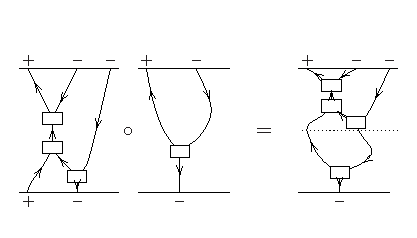
\includegraphics{fig-001}
  \end{equation*}
  \caption{Composition product of RT-diagrams.}
  \label{fig:graph-composition}
\end{figure}
\begin{figure}[tbp]
  \begin{equation*}
    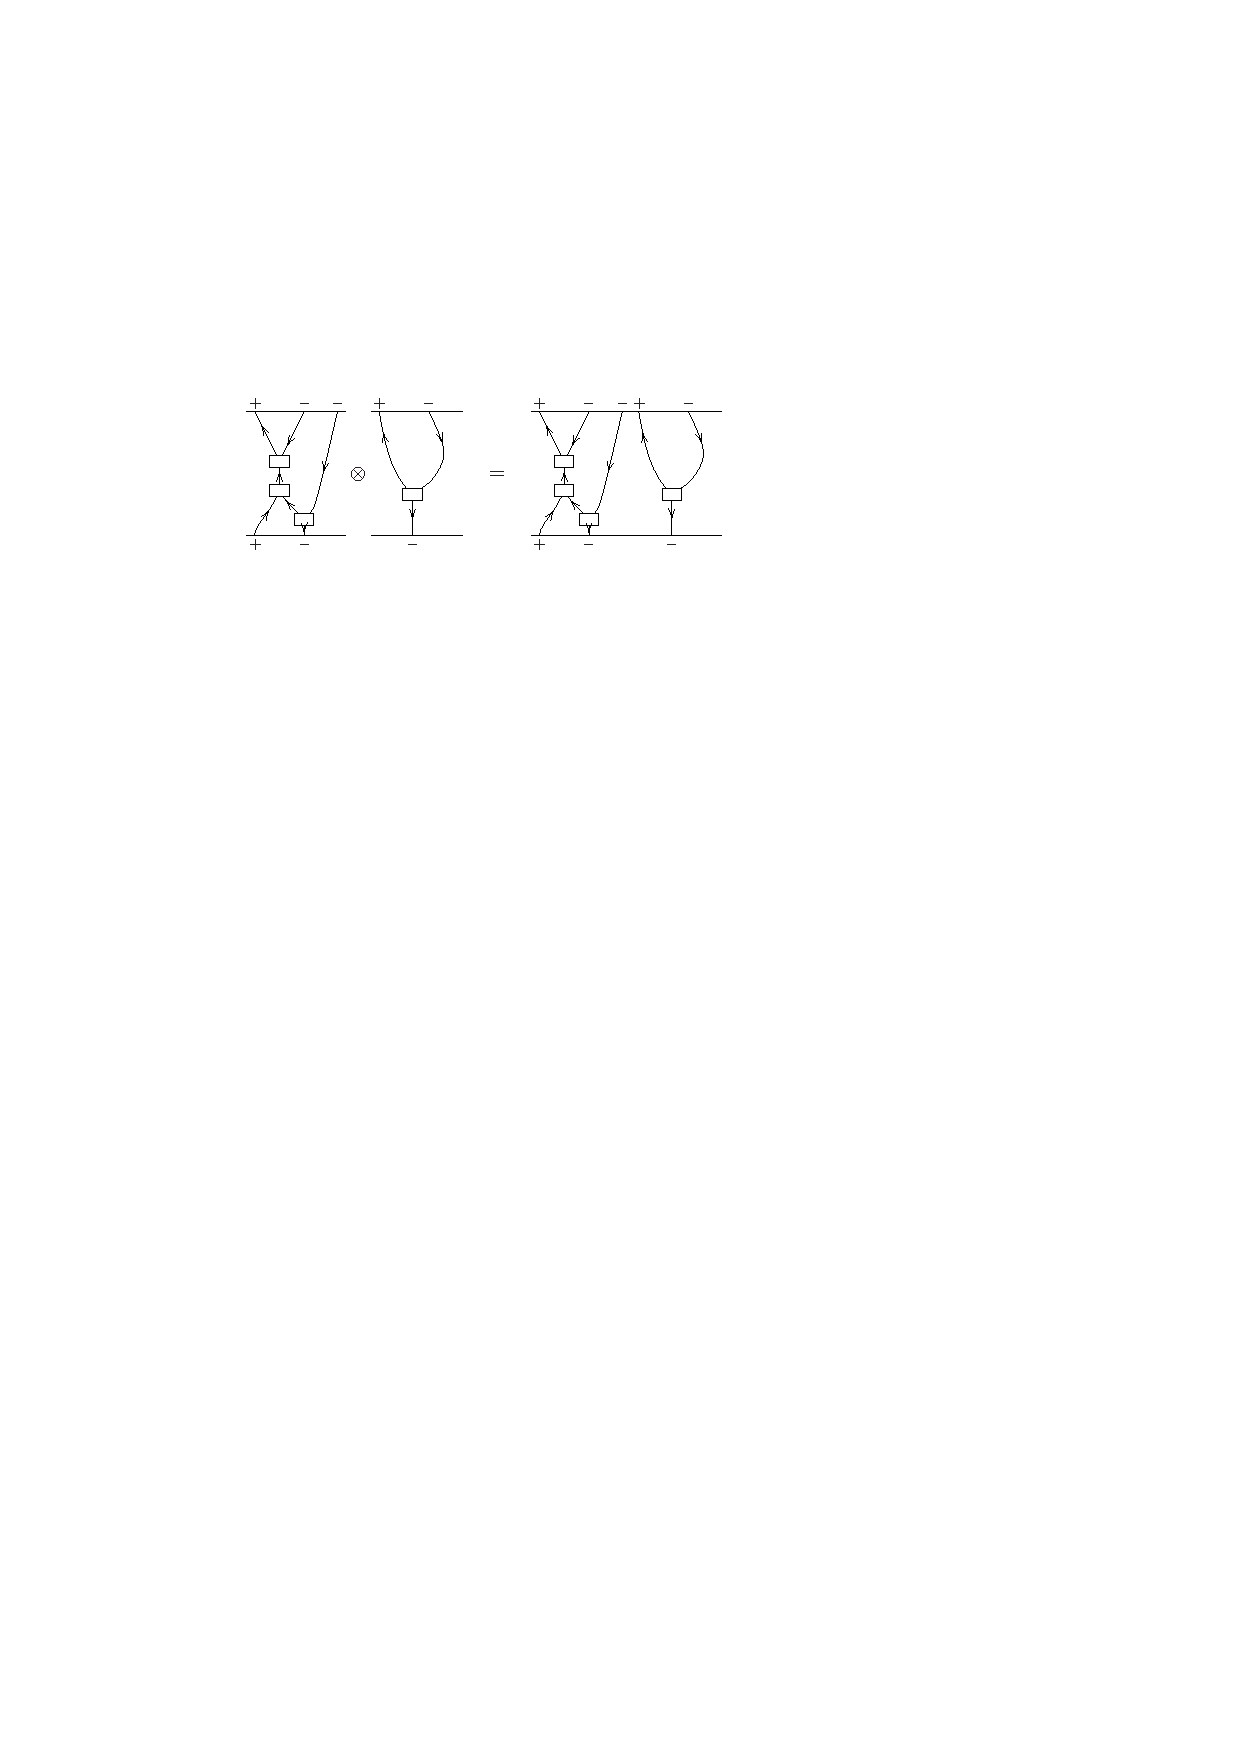
\includegraphics{fig-002}
  \end{equation*}
\caption{Tensor product of RT-diagrams.}
\label{fig:graph-otimes}
\end{figure}

Diagrams corresponding to directed braids on $n$  strands form a group
under the composition product, isomorphic to the semidirect product
$B_n \ltimes \setZ_2^n$.

By the above definitions, we can take the linear spans $\RTD(S,T)$ of
diagrams with given source $S$ and target $T$, as the $\Hom$-spaces of a
suitable category.
\begin{definition}
\label{dfn:diagrams-category}
$\RTD$ is the monoidal category which has finite sequences of $\pm1$ as
objects; the $\Hom$-space $\RTD(S,T)$ is the linear span of the set of
diagrams with source $S$ and target $T$.

Composition of morphisms is defined by bilinear extension of the
composition product $\circ$ (see \csref{dfn:graph-composition}).

The tensor product is given on objects by concatenation:
\begin{equation*}
  (\varepsilon_1, \ldots, \varepsilon_r) \otimes (\varepsilon'_1, \ldots, \varepsilon'_s) = (\varepsilon_1, \ldots, \varepsilon_r, \varepsilon'_1, \ldots, \varepsilon'_s),
\end{equation*}
and on morphisms by juxtaposition of diagrams (see
\csref{fig:graph-otimes}). 
\end{definition}

The category $\RTD$ is not braided, nor autonomous, nor balanced in
any obvious way: it is the deep result of Reshetikhin-Turaev
\cite{reshetikhin-turaev;ribbon-graphs}, Joyal-Street
\cite{joyal-street;tensor-calculus} and Freyd-Yetter
\cite{freyd-yetter;btc} that a quotient of it enjoys all these
structures; moreover, this result can be enhanced by considering
\emph{colored} graphs, and colors can be taken in any braided
autonomous tortile category.


\section{The category of RT-graphs}
\label{sec:rt-graphs}
Let $\Hom\RTD := \bigcup_{S,T \in \RTD} \RTD(S,T)$ be the set of all
morphisms in the category $\RTD$; $\Hom\RTD$ consists of all possible
RT-diagrams. Any RT-diagram can be considered as the planar projection
of a purely $1$-dimensional CW-complex equipped with some additional
structure.
\begin{definition}
  An (embedded) RT-graph\footnote{What is here called an ``RT-graph''
    corresponds to a ``homogeneous colored directed ribbon graph''
    (HCDR-graph) in the terminology of
    \cite{reshetikhin-turaev;ribbon-graphs}: the ``ribbon'' condition
    has been rephrased in terms of framing here, and the
    ``homogeneity'' is hidden in the requirement that $N_\ell$ satisfy
    $N_\ell(0) = N_\ell(1) = 1$. We do not need CDR-graphs (i.e., not
    homogeneous). Also, since we are ultimately going to consider
    coarser invariants than Reshetikhin and Turaev do, the definition
    of RT-graph has been adapted to suit a more combinatorial
    environment.} $\Gamma$ is a $1$-dimensional CW-complex embedded in $M
  = \setR \times [0,1] \times [0,1]$ together with
  \begin{itemize}
  \item for each edge, a choice of a direction;
  \item for each edge, a choice of a framing;
  \item for each vertev $v$, a partition of half-edges incident to it
    into disjoint totally-ordered subsets $\In(v)$ and $\Out(v)$.
  \end{itemize}
  In addition, we stipulate that $\Gamma \cap \partial M$ is a finite set --- call
  its points the \emph{endpoints} of $\Gamma$.  We say that $\Gamma$ has type
  $(p,q)$ iff $\Gamma \cap \partial M \subseteq \{ s_1, \ldots, s_p \} \cup \{ t_1, \ldots, t_q \}$.
\end{definition}
Extending a classical result of Reidmeister, Reshetikhin and Turaev
proved the following.
\begin{lemma}[\cite{reshetikhin-turaev;ribbon-graphs}]\label{lemma:moves}
  The set $\Hom\RTE$ of all isotopy classes (rel $\partial M$)\FIXME{Se
    dobbiamo considerare isotopie col bordo fisso allora non si pu{\`o}
    tagliare un grafo ad altezza generica\ldots vale la pena di essere
    estremamente precisi su questo punto?} of embedded
  RT-graphs is the quotient of the set $\Hom\RTD$ of RT-diagrams
  with respect to the equivalence relation generated by a finite set
  of graphical moves (Reidmeister-Reshetikhin-Turaev moves, see
  \csref{fig:rrt} or \cite{reshetikhin-turaev;ribbon-graphs} for a
  listing).
\end{lemma}
Henceforth, we say ``RT-graph'' to mean an element of $\Hom\RTE$ or an
isotopy class of embedded RT-graphs.\footnote{Reshetikhin and Turaev's
  original definition involved graphs with coupons (i.e., rectangles
  with a pair of preferred edges) as vertices and ribbons as the
  edges. Since the width of ribbons and the size of coupons do not
  matter under isotopy, we are ultimately left with $1$-dimensional
  edges with a framing, and with a partition of the edges incident to
  any given vertex.}
\begin{figure}[htbp]
  \centering
  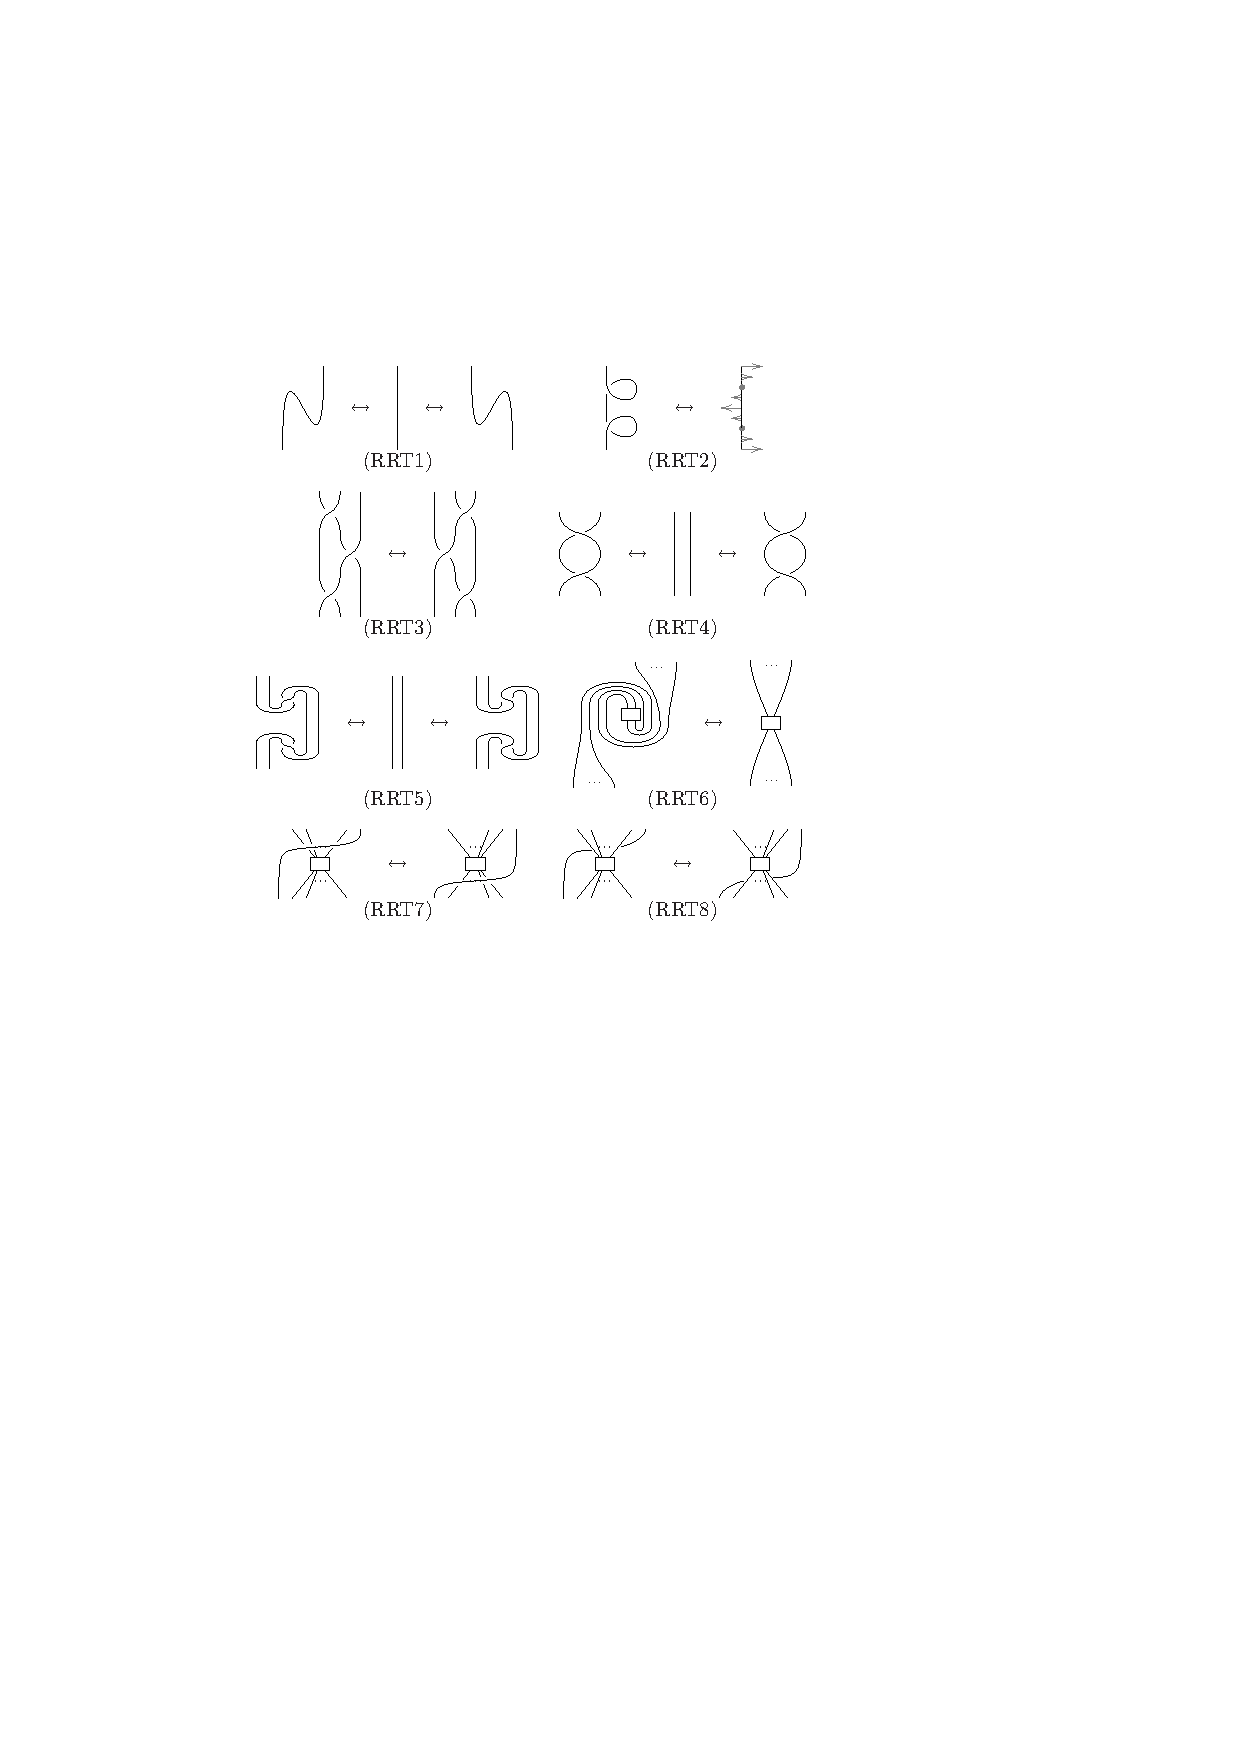
\includegraphics{fig-003}
    \caption{Reidmeister-Reshetikhin-Turaev moves for
      RT-diagrams. Note that move (RRT2) changes a trivial framing
      into a non-trivial (degree $1$) one.}
    \label{fig:rrt}
\end{figure}

It is clear that the operations $\circ$ and $\otimes$ on $\Hom\RTD$ induce
similar composition and tensor product operations on $\Hom\RTE$: any
two RT-graphs can be juxtaposed to form the tensor product $\otimes$ (see
\csref{fig:graph-otimes}) and a pair of graphs with matching input and
output legs can be stacked to form a new RT-graph (see
\csref{fig:graph-composition}).
\begin{lemma}[{\cite[lemmas 5.2 and 5.3]{reshetikhin-turaev;ribbon-graphs}}]
\label{thm:generators}
The set $\Hom\RTE$ of RT-graphs is generated thorugh $\circ$ and $\otimes$ from
the following elementary pieces, modulo the
Reidmeister-Reshetikhin-Turaev relations of \csref{fig:rrt} (an
orientation must be added to each strand!):
\begin{center}
  {%
    \begin{tabular}{cccccc}
      $\xy*!LC\xybox{(0,0);(0,1)**\dir{-}}\endxy$
      &
      $\xy*!LC\xybox{%
        \vcross~{(0,1)}{(1,1)}{(0,0)}{(1,0)}}\endxy$
      &
      $\xy*!LC\xybox{%
        \vcross~{(0,0)}{(1,0)}{(0,1)}{(1,1)}}\endxy$
      &
      $\xy*!LC\xybox{%
        \vloop~{(0,1)}{(1,1)}{(0,0)}{(1,0)}}\endxy$
      &
      $\xy*!LC\xybox{%
        \vloop~{(0,0)}{(1,0)}{(0,1)}{(1,1)}}\endxy$
      &
      $\xy*!LC\xybox{
        (0,1)*+[F]{\ };%
        (-1,0)**\dir{-},(-0.5,0)**\dir{-},%
        (0,0.5)*+{\ldots},(1,0)**\dir{-},%
        (-1,2)**\dir{-},(-0.5,2)**\dir{-},%
        (0,1.5)*+{\ldots},(1,2)**\dir{-},%
        }\endxy$
      \\
      (a) & (b) & (c) & (d) & (e) & (f)
    \end{tabular}
    }
\end{center}
\end{lemma}
A piece of type (a) is called a ``strand''; those of type (b) and (c)
are named ``crossings''; (d) and (e) are the ``coupling'' and the
``Casimir''; (f) is, plainly, a ``vertex''.
\begin{remark} \csref{thm:generators} just states that an
  RT-diagram is a composition of ``rows'' made of pieces of type
  (a)--(f). Generically, such rows will be made of one piece of type
  (b)--(f) padded with a number of strands (a) on the two sides.
\end{remark}

\begin{definition}
  $\RTE$ is the monoidal category whose arrows are elements of
  $\Hom\RTE$ with the composition law and tensor product induced as a
  quotient of $\Hom\RTD$.
\end{definition}
By the arrows-only description of a category (see \csref{cha:arrows}),
we can deduce that objects in $\RTE$ are finite sequences of signs $\pm1$.
Note that, for any such sequence $S$, the set $\RTE(S,S)$ contains the
directed braids group $B_n \ltimes \setZ_2^n$, so any braid is an
isomorphism in $\RTE$.

The category $\RTE$ has duals: for each object $S$, let $\rdl{S}$ be
the sequence obtained from $S$ by flipping it and reversing all the
signs ---for instance, if $S = (+--)$ then $\rdl{S} = (++-)$---; let
$\ev_S: S\otimes\rdl{S} \to I$ be the only graph which connects corresponding
signs in $S$ and $\rdl{S}$ and has only local maxima of the height
function as critical points (see \textsl{(b)} in \csref{fig:struct}),
finally, let $\coev_S : I \to \rdl{S} \otimes S$ be the graph obtained by
flipping $\ev_S$ (see \textsl{(a)} in \csref{fig:struct}).

The category $\RTE$ is balanced by the family of isomorphisms $\theta_S: S
\to S$ defined by requiring that $\theta_{S\otimes T} := \theta_S \otimes \theta_T$ and
that $\theta_{(+)}$ be the straight line $\ell: [0,1] \ni t \mapsto (0,t,0) \in M$
with the degree $1$ framing $N_\ell: [0,1] \ni u \mapsto \exp 2\pi\I u \in
S^1$. (See \textsl{(c)} in \csref{fig:struct}.)

Finally, $\RTE$ is braided by the family of isomorphisms $\tau_{S,T}$
that swap the positions of $S$ and $T$, with directions chosen so to
match the signs on endpoints. (See \textsl{(d)} in
\csref{fig:struct}.)

\begin{figure}[thbp]
  \centering
  \begin{tabular}{cc}
    {\begin{tabular}{cc}
        $\rdl{S} \otimes S$
        &
        $\overbrace{\hspace{1.5cm}}^{\rdl{S}} \hspace{0.5cm}
        \overbrace{\hspace{1.5cm}}^S$
        \\
        ${\xy<0.5cm,0cm>:0, \ar(0,0);(0,3.5) ^{\coev_S} 
          _{\phantom{\coev_S}} \endxy}$
        &
        
\includegraphics[scale=0.5]{coev}
        \\
        $I$
        &
      \end{tabular}}
    &
    {\begin{tabular}{cc}
        $I$
        &
        \\
        $\xy<0.5cm,0cm>:0, \ar(0,0);(0,3.5) ^{\ev_S} _{\phantom{\ev_S}} \endxy$
        &
        
\includegraphics[scale=0.5]{ev}
        \\
        $S \otimes \rdl{S}$
        &
        $\underbrace{\hspace{1.5cm}}_{S} \hspace{0.5cm}
        \underbrace{\hspace{1.5cm}}_{\rdl{S}}$
      \end{tabular}}
    \\
    \textsl{(a)}
    &
    \textsl{(b)}
    \\[12pt]
    {\begin{tabular}{cc}
        S
        &
        S
        \\
        ${\xy<0.75cm,0cm>:0, 
          \ar(0,0);(0,3) ^{\theta_S} _{\phantom{\theta_S}}
          \endxy}$
        &
        ${\xy<1.125cm,0cm>:0,%
          (0,0);(0,2)**\dir{-},
          \ar@[grey] (0,0.00);(+0.50,0.00),
          \ar@[grey] (0,0.25);(+0.25,0.25),
          \ar@{-} (0,0.50)*[grey]{\bullet};(0,0.50),
          \ar@[grey] (0,0.75);(-0.25,0.75),
          \ar@[grey] (0,1.00);(-0.50,1.00),
          \ar@[grey] (0,1.25);(-0.25,1.25),
          \ar@{-} (0,1.50)*[grey]{\bullet};(0,1.50),
          \ar@[grey] (0,1.75);(+0.25,1.75),
          \ar@[grey] (0,2.00);(+0.50,2.00),
          (1,1.5)*{\ldots},
          (2,0);(2,2)**\dir{-},
          \ar@[grey] (2,0.00);(2.50,0.00),
          \ar@[grey] (2,0.25);(2.25,0.25),
          \ar@{-} (2,0.50)*[grey]{\bullet};(2,0.50),
          \ar@[grey] (2,0.75);(1.75,0.75),
          \ar@[grey] (2,1.00);(1.50,1.00),
          \ar@[grey] (2,1.25);(1.75,1.25),
          \ar@{-} (2,1.50)*[grey]{\bullet};(2,1.50),
          \ar@[grey] (2,1.75);(2.25,1.75),
          \ar@[grey] (2,2.00);(2.50,2.00),
          \endxy}$
        \\
        S
        &
        S
      \end{tabular}}
    &
    {\begin{tabular}{cc}
        $T\otimes S$
        &
        $\overbrace{\hspace{1.5cm}}^T \hspace{0.75cm}
        \overbrace{\hspace{1.5cm}}^S$
        \\
        $\xy<0.75cm,0cm>:0, \ar(0,0);(0,3) ^{\tau_{S,T}} _{\phantom{\tau_{S,T}}} \endxy$
        &
        
\includegraphics[scale=0.75]{braid}
        \\
        $S\otimes T$
        &
        $\underbrace{\hspace{1.5cm}}_S \hspace{0.75cm}
        \underbrace{\hspace{1.5cm}}_T$
      \end{tabular}}
    \\
    \textsl{(c)}
    &
    \textsl{(d)}
  \end{tabular}
  \caption{The structure morphisms making $\RTE$ into a braided \textsl{(d)},
    autonomous \textsl{(a, b)}, tortile \textsl{(c)} category. The
    directions on each strand must be chosen according to the signs in
    $S$ and $T$. Note that the balancing $\theta_S$ is just the identity
    with a different framing.}
  \label{fig:struct}
\end{figure}

\begin{proposition}\label{thm:rt}
  The category $\RTE$ is braided, autonomous, and tortile.
\end{proposition}
\begin{proof}
  All the verifications reduce to checking that some RT-graph
  corresponding to a composition of the strcture morphisms is
  \emph{isotopic} to some other RT-graph, again composition of the
  structure morphisms ---for instance, move (RRT1) in \csref{fig:rrt}
  is the verification that $(\ev_{(\pm)}, \coev_{(\pm)})$ is a duality
  pair--- and this is easily done.
\end{proof}


\section{Graphical calculus on tortile braided tensor categories}
\label{sec:rt-gc}
Now let $\A$ be a tensor category. Define $\freemsc{\A}$ to be the
category whose objects are finite sequences $(A_1, \ldots, A_r; \varepsilon_1, \ldots,
\varepsilon_r)$ of objects in $\A$ and signs $\pm1$, whereas a morphism $(A_*,
\varepsilon_*) \to (B_*, \delta_*)$ is an element $f \in \A(A_1^{\varepsilon_1} \otimes \ldots \otimes
A_r^{\varepsilon_r}, B_1^{\delta_1} \otimes \ldots B_s^{\delta_s})$ --- recall that $A^1 = A$
and $A^{-1} = \rdl{A}$.  There is an obvious functor $\freemsc{\A} \to
\A$ defined on objects by $(A_1, \ldots, A_r; \varepsilon_1, \ldots, \varepsilon_r) \mapsto
A_1^{\varepsilon_1} \otimes \cdots \otimes A_r^{\varepsilon_r}$.
\begin{definition}
  An $\A$-colored RT-diagram $\Gamma$ is an RT-diagram together with:
  \begin{enumerate}
  \item an assignment of an object $A_\ell \in \A$ for each
    $\ell\in\Edges{\Gamma}$;
  \item an assignment of a morphism $f\in\A(\Src(v),\Tgt(v))$ for each
    vertex $v$ of $\Gamma$, where $\Src(v)$ and $\Tgt(v)$ are the
    sequences $(A_1, \ldots, A_r;\varepsilon_1, \ldots, \varepsilon_r)$ of objects and signs
    decorating edges in $\In(v)$ and $\Out(v)$.
  \end{enumerate}
  The source and the target of an $\A$-colored RT-diagram are defined
  analogously and are denoted $\Src_\A(\Gamma)$ and $\Tgt_\A(\Gamma)$ respectively.
\end{definition}
It is trivial to generalize \csref{dfn:diagrams-category} to
$\A$-colored RT-diagrams.
\begin{definition}
  The category of $\A$-colored RT diagrams $\RTD[\A]$  has
  $\freemsc{A}$ as its set of objects and $\A$-colored RT-diagrams as
  morphisms. 
\end{definition}
For each $\A$-colored RT-diagram $\Gamma$, $\Src{}_{\A}(\Gamma)$ and
$\Tgt{}_{\A}(\Gamma)$ are objects of $\freemsc{\A}$.  Obviously, $\circ$ and
$\otimes$ are bilinear with respect to the vector space structure on the
$\Hom$-sets of $\RTD[\A]$. Any $\A$-colored RT-diagram can be seen as
the planar projection of an $\A$-colored RT-graph and the following
analogue of lemma \ref{thm:generators} hold.
\begin{proposition}
\label{thm:rt1}
The set $\Hom\RTD[\A]$ of $\A$-colored RT-diagrams is generated thorugh
$\circ$ and $\otimes$ from the following elementary pieces (an orientation
must be added to each strand!):
\begin{center}
  {%
    \begin{tabular}{cccccc}
      $\xy*!LC\xybox{(0,0)*+{A};(0,1)*+{A}**\dir{-}}\endxy$
      &
      $\xy*!LC\xybox{%
        \vcross~{(0,1)*+{B}}{(1,1)*+{A}}{(0,0)*+{A}}{(1,0)*+{B}}}\endxy$
      &
      $\xy*!LC\xybox{%
        \vcross~{(0,0)*+{B}}{(1,0)*+{A}}{(0,1)*+{A}}{(1,1)*+{B}}}\endxy$
      &
      $\xy*!LC\xybox{%
        \vloop~{(0,1)}{(1,1)}{(0,0)*+{A}}{(1,0)*+{A}}}\endxy$
      &
      $\xy*!LC\xybox{%
        \vloop~{(0,0)}{(1,0)}{(0,1)*+{A}}{(1,1)*+{A}}}\endxy$
      &
      $\xy*!LC\xybox{
        (0,1)*+[F]{f};%
        (-1,0)*+{A_1}**\dir{-},(-0.5,0)*+{A_2}**\dir{-},%
        (0,0.5)*+{\ldots},(1,0)*+{A_r}**\dir{-},%
        (-1,2)*+{B_1}**\dir{-},(-0.5,2)*+{B_2}**\dir{-},%
        (0,1.5)*+{\ldots},(1,2)*+{B_s}**\dir{-},%
        }\endxy$
      \\
      (a) & (b) & (c) & (d) & (e) & (f)
    \end{tabular}
    }
\end{center}
The set $\Hom\RTE[\A]$ of $\A$-colored RT-graphs is the quotient of
$\Hom\RTD[\A]$ with respect to the Reidmeister-Reshetikhin-Turaev
relations of \csref{fig:rrt}.
\end{proposition}

Let $\category{B}$ be a tensor category. A tensor functor
$\RTD[\A]\to{\category{B}}$ is uniquely specified if we define it on
the generators; it induces a tensor functor $\RTE[\A] \to \category{B}$
if it is compatible with relations (RRT1)--(RRT8).  In particular,
taking $\category{B}=\A$ we find the following.
\begin{theorem}[Reshetikhin-Turaev,
  \cite{reshetikhin-turaev;ribbon-graphs}]
  \label{thm:rt2}
  For any autonomous balanced braided tensor category $\A$, there is a
  tensor functor $Z_{\A}: \RTD[\A] \to \A$, mapping an object $(A_1,
  \ldots, A_k; \varepsilon_1, \ldots, \varepsilon_k) \in \RTD[\A]$ to $A_1^{\varepsilon_1} \otimes \dots \otimes
  A_k^{\varepsilon_k} \in \A$, and defined on generators of morphisms in
  $\RTD[\A]$ by
\begin{center}
  \everyxy={/r24pt/:}
  {%
    \begin{tabular}{ccc}
      $\xy*!LC\xybox{%
        \vcross~{(0,1)*+{B}}{(1,1)*+{A}}{(0,0)*+{A}}{(1,0)*+{B}}}\endxy
      \mapsto \tau_{XY},$
      %\label{graph-cross+}
      &
      $\xy*!LC\xybox{%
        \vcross~{(0,0)*+{B}}{(1,0)*+{A}}{(0,1)*+{A}}{(1,1)*+{B}}}\endxy
      \mapsto \tau_{XY}^{-1},$
      %\label{graph-cross-}
      &
      $\xy*!LC\xybox{
        (0,1)*+[F]{f};%
        (-1,0)*+{A_1}**\dir{-},(-0.5,0)*+{A_2}**\dir{-},%
        (0,0.5)*+{\ldots},(1,0)*+{A_r}**\dir{-},%
        (-1,2)*+{B_1}**\dir{-},(-0.5,2)*+{B_2}**\dir{-},%
        (0,1.5)*+{\ldots},(1,2)*+{B_s}**\dir{-},%
        }\endxy \mapsto f$
      %\label{graph-morphism} 
      \\
      $\xy*!LC\xybox{%
        \vloop~{(0,1)}{(1,1)}{(0,0)*+{A}}{(1,0)*+{A}}}\endxy \mapsto
      \ev_{A},$
      %\label{graph-casimir}
      &
      $\xy*!LC\xybox{%
        \vloop~{(0,0)}{(1,0)}{(0,1)*+{A}}{(1,1)*+{A}}}\endxy \mapsto
      \coev_{A},$
      %\label{graph-coupling}
      &
      $\xy*!LC\xybox{(0,0)*+{A};(0,1)*+{A}**\dir{-}}\endxy \mapsto
      \id_X,$
      %\label{graph-id}
    \end{tabular}
    }
  \end{center}
where $\tau_{AB}$, $\ev_A$, $\coev_A$ are the structure maps in
$\A$, and $f$ is a morphism in $\A$; take the dual of an
object if the sign $\varepsilon$ on the corresponding edge is $-1$.

The tensor functor $Z_\A$ is invariant by the
Reidmeister-Reshetikhin-Turaev moves (RRT1)--(RRT8), so it induces a
faithful\FIXME{Non sono proprio sicuro che sia fedele!} tortile
braided functor $Z_\A: \RTE[\A] \to \A$.
\end{theorem}
\begin{remark}
By definition of a tensor functor, the following relations hold:
\begin{gather*}
  Z_{\A}(\Gamma\circ\Phi) = Z_{\A}(\Gamma) \circ Z_{\A}(\Phi), 
  \qquad 
  Z_{\A}(\Gamma\otimes\Phi) = Z_{\A}(\Gamma) \otimes Z_{\A}(\Phi),
  \\
  Z_{\A}(a\Gamma + b\Phi) = aZ_{\A}(\Gamma) + bZ_{\A}(\Phi).
\end{gather*}
\end{remark}

%%% Local Variables: 
%%% mode: latex
%%% TeX-master: "index"
%%% x-symbol-8bits: nil
%%% End: 




%% 
%% Indice dei simboli
%%
\printglossary


%%
%% Bibliografia
%%
\bibliography{math}
\bibliographystyle{halpha}


\end{document}

%%% Local Variables: 
%%% mode: latex
%%% TeX-master: t
%%% x-symbol-mode: nil
%%% End: 
